%% main.tex — Paper 2 (xai_2_interpretability) master document.
%% Built from the Springer Nature sn-jnl class (sn-article-SAMPLE.tex as reference).
%% Target: Nature Machine Intelligence (Nature Portfolio) — Article/Analysis.
%%
%% SCRUM note: this master \input{}s one file per section. Each per-section file is
%% owned by a single writing item (P2-E8-1 .. P2-E8-9) so they can be drafted in
%% parallel without colliding (SCRUM §6 disjoint file_scope). Do NOT inline section
%% bodies here. All drafting follows ../STYLE.md (Andreas Maier's voice).
%%
%% NOTE on the SN single-file rule: the SN sample says "do not use \input{...}".
%% That rule governs the *final submission package* (one .tex for production XML).
%% For drafting we keep sections split; a flatten step at submission time inlines them.

%% Style for submissions to Nature Portfolio journals (NMI is Nature Portfolio).
%% pdflatex option: compile with pdflatex/xelatex.
\documentclass[sn-nature,pdflatex]{sn-jnl}

%%%% Standard packages
\usepackage{graphicx}%
\usepackage{multirow}%
\usepackage{amsmath,amssymb,amsfonts}%
\usepackage{amsthm}%
\usepackage{mathrsfs}%
\usepackage[title]{appendix}%
\usepackage{xcolor}%
\usepackage{textcomp}%
\newcommand{\Sectionname}{Section~}%
\usepackage{manyfoot}%
\usepackage{booktabs}%
\usepackage{algorithm}%
\usepackage{algorithmicx}%
\usepackage{algpseudocode}%
\usepackage{listings}%

%% Figures live in figures/ (fig1..fig6 PDFs already generated there).
\graphicspath{{figures/}}

%% Theorem environments (the F and S and M triad / definitions go here).
\theoremstyle{thmstyleone}%
\newtheorem{theorem}{Theorem}%
\newtheorem{proposition}[theorem]{Proposition}%
\theoremstyle{thmstyletwo}%
\newtheorem{example}{Example}%
\newtheorem{remark}{Remark}%
\theoremstyle{thmstylethree}%
\newtheorem{definition}{Definition}%

\raggedbottom

%% sn-jnl + hyperref emit each float's PDF destination twice at its own location
%% (pdftex "destination with the same identifier (figure.N)"). hypertexnames=false makes
%% hyperref name anchors by an internal serial counter, so the doubled emission cannot
%% collide. Cross-references and citation links are unaffected. Set after the class has
%% loaded hyperref.
\AtBeginDocument{\hypersetup{hypertexnames=false}}

\begin{document}

%%=============================================================%%
%% Title — reframed (declarative-claim register, Maier/Nature-family):
%% the title states the *result*, not the artifact.
%%=============================================================%%
\title[Faithful attribution recovers the causal wiring, not the semantics]{Faithful attribution recovers the causal wiring, not the semantics: a ground-truth audit of interpretability on a differentiable microprocessor}

%%=============================================================%%
%% Authors (provisional) — A. Maier et al.
%%=============================================================%%
\author*[1]{\fnm{Andreas} \sur{Maier}}\email{andreas.maier@fau.de}

\author[1]{\fnm{Siming} \sur{Bayer}}

\author[1]{\fnm{Patrick} \sur{Krauss}}

\affil*[1]{\orgdiv{Pattern Recognition Lab}, \orgname{Friedrich-Alexander-Universit\"at Erlangen-N\"urnberg}, \orgaddress{\city{Erlangen}, \country{Germany}}}

%%=============================================================%%
%% Abstract + keywords (body drafted in sections/00_abstract.tex)
%%=============================================================%%
\abstract{% 00_abstract.tex — Abstract. Drafted by item P2-E8-1.
% Body only: this file is \input{} inside \abstract{...} in main.tex (no \section).
% NMI rule (document_check.md C): UNREFERENCED abstract — no \cite — and ~150-200 words.
% Maier/NMI voice per ../STYLE.md; honesty contract per ../plan.md.
We ask whether a faithful explanation is already an understanding.
Interpretability methods are judged by their faithfulness --- whether they name
the true causes --- yet on real neural systems there is no ground truth against
which to check them. We remove that excuse on a system whose ground truth is
computable: a bit-exact, differentiable port of the Atari~2600, never built to be
interpretable, in which the cause of any output follows from exact intervention.
Scoring about~31 interpretability methods against this oracle, we find causal
methods faithful, while popular gradient and correlational saliency methods are
provably zero on discrete position outputs (activation patching $1.000$ versus
vanilla saliency $0.000$) yet score higher on human plausibility --- a danger
zone of conviction without correctness. Yet
faithfulness is the smaller half of understanding: an exact method returns a
causal-effect map or a data-flow graph, not the computation. A graph-correct
circuit need not reproduce behavior (sufficiency $0.44$), and a feature matching a
named variable can be causally inert (matched fraction $1.0$,
faithfulness $0.04$). We name this measured
residual the \emph{semantic gap}, and stress that we \emph{measure} it, not
\emph{close} it. As such, the approach offers a reusable ground-truth benchmark
for explainable AI, mechanistic interpretability, AI safety, and software
verification. We assume that it will help redirect the field toward recovering
meaning, not merely confirming causes.

% BIBTEX-NEEDED: (none) — the abstract is intentionally citation-free per the NMI
%   unreferenced-abstract rule (document_check.md C). No \cite keys introduced;
%   references.bib unchanged.
}

\keywords{interpretability, explainable AI, mechanistic interpretability, faithfulness, ground truth, causal attribution, semantic gap, Atari VCS}

\maketitle

%%=============================================================%%
%% Body — one \input per section (Nature Article order):
%% Introduction (unnumbered lead, with Related work folded in) ->
%% Results (A, B, C, comparison) -> Discussion -> Methods -> End-matter.
%% Related work (02_related) is folded into the Introduction (01_intro)
%% and is no longer \input here.
%%=============================================================%%
% 01_intro.tex — Introduction (Nature Article lead; Related work folded in).
% Maier voice per ../STYLE.md (plain, precise, short sentences; no poetic register).
% The Introduction is the unnumbered lead right after the abstract (Nature Article
% format), so it carries no \section heading.
% Arc (each point stated ONCE): problem (faithfulness, unmeasurable) -> the three
%  traditions share the blind spot -> the oracle makes it measurable (Fig 1) ->
%  result 1: faithfulness measured -> result 2: the faithfulness escape removed
%  (sampler on), the gap survives -> the semantic gap, both directions, F/S/M ->
%  meaning's reference is behaviour -> contributions and scope.
% Detailed benchmark comparison (BAM/M4/Tracr/InterpBench/MIB), the Atari-environment
% lineage, and the competing definitions of "interpretable" (Barbiero; Marr; Lazebnik)
% live in the Discussion to avoid repeating them here; every \cite key is preserved
% across the two sections (see the whole-paper citation check in the rework commit).
% Numbers: sampler from compare/out/sampler_faithfulness.csv (R7-1); rest from number_audit §1.

Interpretability now matters in practice. Neural networks drive cars, read scans, and
approve loans. Before we trust such a decision, we ask why. Yet on the systems we most
want to explain we cannot check whether the answer is correct. A saliency map for a deep
network can look convincing and can change with the action, and still not be a correct
explanation~\cite{greydanus2018visualizing}. The field of explainable AI has converged on
\emph{faithfulness} as its quality criterion: whether an explanation names a system's
\emph{true} causes~\cite{jacovi2020towards}. The difficulty is that on a real neural
network there is nothing to measure it against. Sanity checks can show that a method fails,
but with no reference map they cannot certify that it is correct~\cite{adebayo2018sanity}.

This blind spot is not specific to deep learning. Jonas and Kording applied standard
neuroscience methods to a microprocessor in which every transistor is
known~\cite{jonas2017could}. Lesions, tuning curves, and connectomics produced rich
structure, but none of it recovered how the chip computes. The same gap recurs across the
three interpretability traditions that rarely cite one another. The neuroscience battery
records and perturbs a system. The attribution tradition asks which inputs mattered for a
decision, through gradient and saliency
maps~\cite{simonyan2014deep,sundararajan2017axiomatic,smilkov2017smoothgrad,springenberg2015striving},
class-activation methods~\cite{selvaraju2017gradcam,chattopadhyay2018gradcampp},
occlusion~\cite{zeiler2014visualizing,fong2017interpretable,petsiuk2018rise}, and surrogate
or game-theoretic attributions~\cite{ribeiro2016why,lundberg2017unified}, applied to Atari
agents to visualise what a policy attends~\cite{greydanus2018visualizing,such2019atarizoo}.
Mechanistic interpretability aims past attribution at the circuit, through path patching and
causal mediation~\cite{vig2020investigating,meng2022locating,wang2022interpretability,conmy2023towards},
alignment search and interchange interventions~\cite{geiger2021causal,geiger2023finding}, and
the sparse dictionaries and probes that read features off the
state~\cite{cunningham2023sparse,alain2017understanding,hewitt2019designing,belrose2023eliciting,nanda2023attribution}.
Across all three, methods are validated against each other or against human intuition rather
than against the mechanism~\cite{atrey2020exploratory}, and even the sparse-dictionary branch
reports that its tuning proxies do not track interpretability~\cite{saebench2025}.
Faithfulness has stood in for understanding, and no one could test the stand-in.

Maier et al. recently built the missing reference. It is a bit-exact, differentiable port
of the Atari 2600 Video Computer System (VCS) that reproduces a real 1977 machine to the
byte and pixel~\cite{maier2025vcs,xitari}. The VCS is software with a known specification,
so the true cause of any output is computable by exact intervention. This \emph{intervention
oracle} (\Sectionname\ref{sec:oracle}) returns the true causal effect for any candidate
cause of any output, measured rather than estimated. It operates over the platform shown in
Fig.~\ref{fig:platform}. On this machine an interpretability claim can be scored right or
wrong. We operationalise interpretability as ground-truth recovery: an explanation is
interpretable to the degree that its claimed structure matches the system's true causal
structure, scored by the oracle.

\begin{figure}[t]
  \centering
  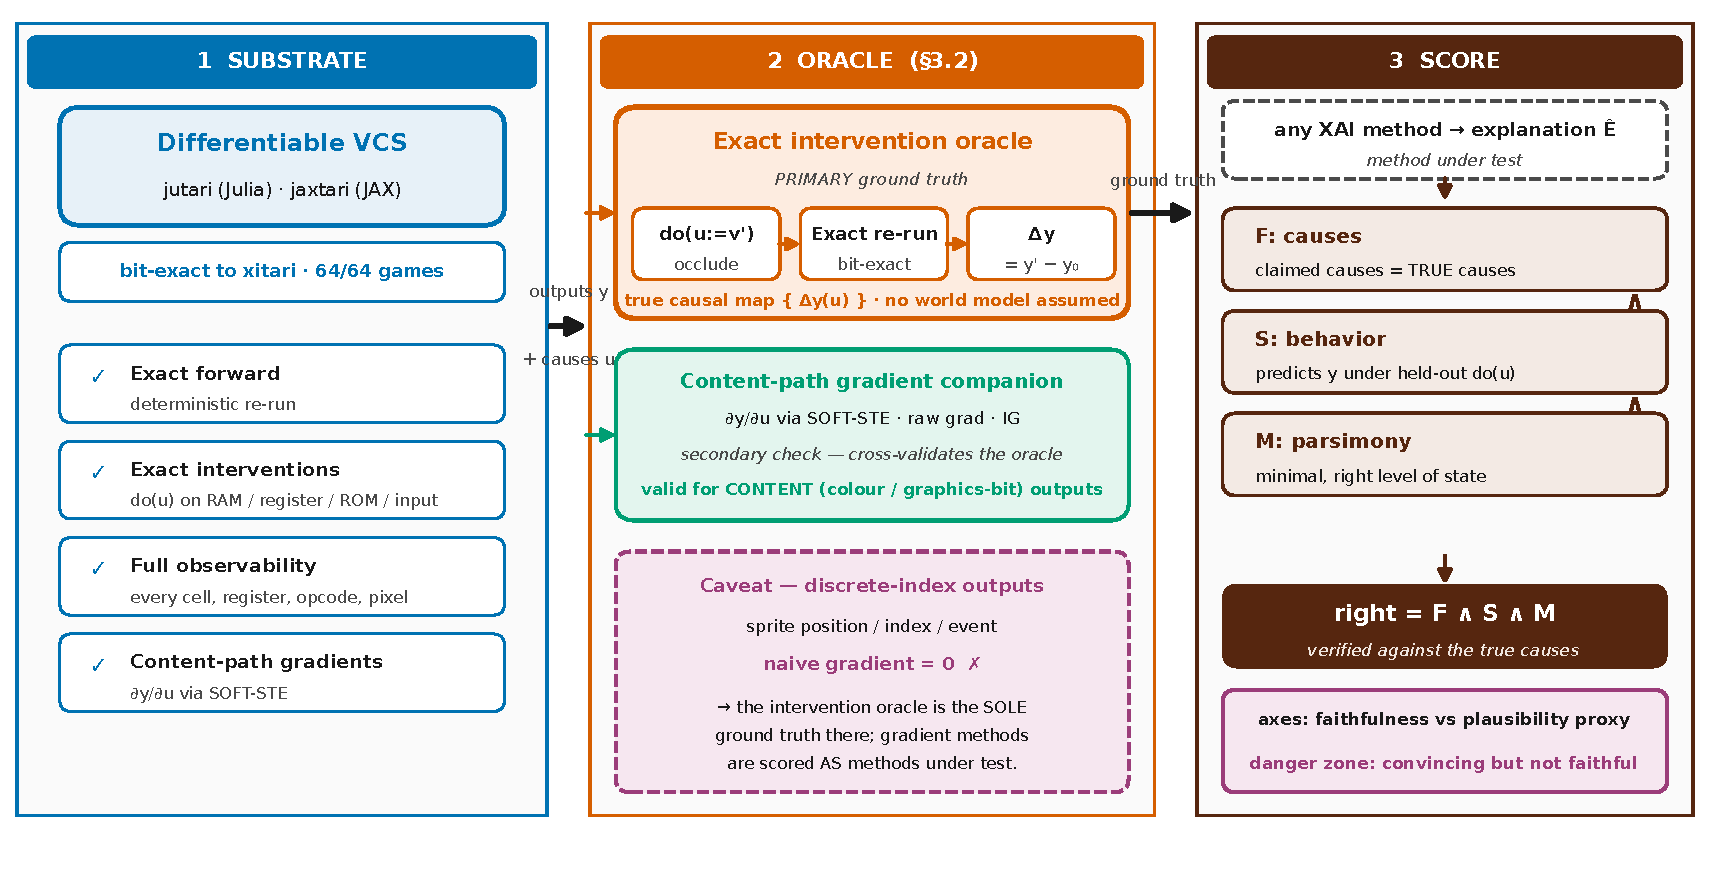
\includegraphics[width=\linewidth]{fig1_platform_oracle.pdf}
  \caption{\textbf{The measurement platform and its ground-truth oracle.} A
  differentiable, bit-exact port of the Atari VCS (left), realized as
  \texttt{jutari} (Julia) $\cdot$ \texttt{jaxtari} (JAX), gives four capabilities no neural
  network grants for free: exact forward, exact interventions $\mathrm{do}(u)$, full state
  observability, and content-path gradients. On it we build the oracle (centre): the primary
  intervention oracle of \Sectionname\ref{sec:oracle}, $\mathrm{do}(u{:=}v')\!\to\!\Delta y(u)$
  by bit-exact re-run, with a content-path gradient $\partial y/\partial u$ as a companion on
  the content path only. Any explanation $\hat{E}$ is scored by the correctness triad (right),
  $\text{right}=\mathrm{F}\wedge\mathrm{S}\wedge\mathrm{M}$, and reported on two axes,
  faithfulness against the oracle versus a plausibility proxy. Faithfulness aggregates
  correlation, sign and magnitude agreement, deletion/insertion area-under-curve, and
  precision at $k$ against the true causal top-$k$ (\Sectionname\ref{sec:triad}). A discrete index --- a
  sprite's position, set by strobe timing --- has a naive gradient that is zero under the hard
  forward map (Prop.~\ref{prop:zero}); for position, index, and event outputs the intervention
  oracle is the \emph{sole} ground truth and gradient methods are scored as methods under test.
  The schematic draws no experiment data. Data and oracle: see Supplement; oracle defined in
  \Sectionname\ref{sec:oracle}.}
  \label{fig:platform}
\end{figure}

We audit $30$ interpretability methods plus the oracle positive control, across $31$
experiments and $257$ per-game records, scoring each on two axes: faithfulness against the
oracle, and a documented plausibility proxy for how convincing it looks. The first result is
the expected one. Causal and intervention methods are faithful; gradient and correlational
saliency methods are not. The contrast is sharpest on discrete sprite-position outputs, where
the naive gradient is provably zero because position is set by strobe timing rather than by a
value it can flow through. There activation patching~\cite{vig2020investigating,meng2022locating}
reaches faithfulness $1.000$ while vanilla saliency~\cite{simonyan2014deep} collapses to
$0.000$ on all six core games~\cite{faithfuldemoP2}, and the leaderboard plots all $31$ methods
against the same ground truth (Fig.~\ref{fig:faithfulness})~\cite{leaderboardP2}. The saliency
method nonetheless carries the higher plausibility score ($0.9$ versus $0.5$): it looks most
convincing exactly where it is least correct. This is the result the field would predict, and
we treat it as an intermediate step, not the main finding.

Faithfulness is not what separates good explanations from bad ones. A reader could dismiss the
zero of the gradient methods as a fixable artifact of a discrete index, so we test the
strongest version of the question and close that objection. We turn the differentiable port's
bilinear sampler on. The sampler interpolates the position read and restores a non-zero
gradient through it, and the gradient methods become faithful too. Vanilla saliency,
grad$\times$input, smoothgrad, and expected gradients reach $0.791$ on Pong, and the same
family reaches $0.529$ on Q*bert (Fig.~\ref{fig:sampler}). The rise is real but not universal:
integrated gradients with a zeros baseline still vanishes on Pong, and a static-sprite game
offers no position to restore. Yet on every game where the gradient becomes faithful, the
method still recovers no meaning, just as no other method does, faithful or not. The restored
gradient concentrates on the position RAM byte that drives the sprite, \texttt{ram[54]} on
Pong. It identifies the correct cause but supplies no meaning for it.

Securing faithfulness is necessary, but it does not solve the main problem. With the same
oracle we ask not only \emph{which} methods are faithful but \emph{what} a faithful method
delivers, and the answer is always the same kind of object: a true causal-effect map or
data-flow graph, never the variable's meaning and never the routine's algorithm. To make this
precise we call an explanation right only if it is \textbf{F}aithful (its claimed causes are
the true ones), \textbf{S}ufficient (it regenerates behavior under held-out interventions),
and \textbf{M}inimal at the algorithmic level
($\mathrm{right} = \mathbf{F}\wedge\mathbf{S}\wedge\mathbf{M}$, \Sectionname\ref{sec:triad}).
The committed data show the gap in both directions (Fig.~\ref{fig:taxonomy}). An automatically
discovered circuit on Breakout is graph-correct and minimal yet reproduces the behavior it
explains only part of the time ($\mathbf{F}=1.0$, $\mathbf{M}=1.0$, $\mathbf{S}=0.44$): a
correct wiring diagram is not the computed function. A learned feature dictionary on Pong
matches a named game variable perfectly (matched fraction $1.0$) while being causally almost
inert ($\mathbf{F}=0.04$): looking like a known variable is not computing it the way the
program does. A concept can be linearly decodable yet provably unused; being present in the
state is not being used. We name this residual the \emph{semantic gap}, and it does not shrink
when faithfulness is made universal.

The reference for meaning lies outside the mechanism. Every semantic label in the study entered
from outside the system, imported from external annotation
sets~\cite{anand2019unsupervised,delfosse2023ocatari} and only \emph{causally verified} on our
substrate, never \emph{discovered} by a method under test. An alignment method that reports
perfect accuracy is therefore right by construction, because it checks a variable we supplied.
Probing shows that information is present, not that it is used~\cite{hewitt2019designing}, and
our oracle is the strictly stronger test. What fixes the meaning is the system's
\emph{behavior}. For software, that behavior is set down in its documentation and data: the
manuals, the specification, and the design. IEEE~610.12 makes these part of the definition of
software itself~\cite{ieee610}. The wiring is in the mechanism, so any faithful method can
recover it. The meaning is not, and no method we tested supplied it.

To our knowledge this is the first cross-tradition audit of interpretability methods on a real,
human-written software artifact whose ground truth is independent of it, scored by an exact
intervention oracle. We claim no unqualified ``first ground-truth calibration,'' since
synthetic known-answer benchmarks and Jonas and Kording's microprocessor
study~\cite{jonas2017could} precede us; the Discussion places our oracle against those
benchmarks and against the competing senses of ``interpretable.'' We read a 1977 chip as a
\emph{necessary-condition screen}, not a predictor of success on learned networks. Here we hold
perfect ground truth and no learning obscures the mechanism, so failure under these conditions
is strong negative evidence that the same method would recover causal mechanisms in harder,
less observable systems. The chip still exhibits the properties that make interpretation hard,
from aliased RAM cells to race-the-beam timing.

We are deliberate about what we do not claim. No method recovered the program's meaning,
algorithm, or design from scratch, and the plausibility axis is a documented proxy, not a
human study. This paper \emph{defines and measures} the semantic gap and locates its reference
in the system's behavior. \emph{Closing} the gap means recovering a system's documentation and
design from the system alone. That is future work, hopefully inspired by this paper. The study
thus offers a reusable ground-truth benchmark for explainable AI, mechanistic interpretability,
AI safety, and software verification, and it reframes the open problem. The hard part of
interpretability is not faithfulness. It is recovering meaning, which remains unsolved even when
faithfulness is achieved. We believe that naming and demonstrating the existence of this gap is
a first step toward closing it.


% BIBTEX-NEEDED manifest (provenance for the SM merge; comments only, no typeset effect).
% Keys cited HERE that may need merging into references.bib: maier2025vcs,
% anand2019unsupervised, hewitt2019designing (plus those already present: jonas2017could,
% atrey2020exploratory, greydanus2018visualizing, xitari, delfosse2023ocatari).
% Keys formerly in this section that now live in the DISCUSSION after the intro rework
% (do NOT re-add them here): barbiero2025neural, bellemare2013arcade, machado2018revisiting,
% dalton2020cule, delfosse2025jaxatari (Atari-environment lineage + "interpretable" variants),
% and the benchmark-comparison keys lindner2023tracr, gupta2024interpbench, yang2019bim,
% m4_2023, mib2025, marr1982vision, lazebnik2002can (08_discussion.tex carries them).
%
% @article{jonas2017could,
%   title   = {Could a Neuroscientist Understand a Microprocessor?},
%   author  = {Jonas, Eric and Kording, Konrad Paul},
%   journal = {PLoS Computational Biology},
%   volume  = {13}, number = {1}, pages = {e1005268}, year = {2017},
%   publisher = {Public Library of Science}, doi = {10.1371/journal.pcbi.1005268}}
%
% @inproceedings{atrey2020exploratory,
%   title     = {Exploratory Not Explanatory: Counterfactual Analysis of Saliency Maps for Deep Reinforcement Learning},
%   author    = {Atrey, Akanksha and Clary, Kaleigh and Jensen, David},
%   booktitle = {International Conference on Learning Representations (ICLR)},
%   year      = {2020}}
%
% @inproceedings{greydanus2018visualizing,
%   title     = {Visualizing and Understanding Atari Agents},
%   author    = {Greydanus, Sam and Koul, Anurag and Dodge, Jonathan and Fern, Alan},
%   booktitle = {International Conference on Machine Learning (ICML)},
%   pages     = {1792--1801}, year = {2018}, organization = {PMLR}}
%
% @inproceedings{anand2019unsupervised,
%   title     = {Unsupervised State Representation Learning in Atari},
%   author    = {Anand, Ankesh and Racah, Evan and Ozair, Sherjil and Bengio, Yoshua and C\^{o}t\'{e}, Marc-Alexandre and Hjelm, R Devon},
%   booktitle = {Advances in Neural Information Processing Systems (NeurIPS)},
%   volume    = {32}, year = {2019}}
%
% @inproceedings{delfosse2023ocatari,
%   title     = {OCAtari: Object-Centric Atari 2600 Reinforcement Learning Environments},
%   author    = {Delfosse, Quentin and Bl{\"u}ml, Jannis and Gregori, Bjarne and Sztwiertnia, Sebastian and Kersting, Kristian},
%   booktitle = {Reinforcement Learning Conference (RLC)}, year = {2024},
%   note      = {arXiv:2306.08649}}
%
% @inproceedings{hewitt2019designing,
%   title     = {Designing and Interpreting Probes with Control Tasks},
%   author    = {Hewitt, John and Liang, Percy},
%   booktitle = {Conference on Empirical Methods in Natural Language Processing (EMNLP)},
%   pages     = {2733--2743}, year = {2019}}
%
% @misc{maier2025vcs,
%   title  = {A Bit-Exact, Differentiable Atari 2600 (Paper 1)},
%   author = {Maier, Andreas and Bayer, Stefan and Krauss, Patrick},
%   year   = {2025}, note = {companion paper; this program}}

\section{Results}\label{sec:results}
% 04_results_A.tex — Results A: the neuroscience battery, quantified (P2-E8-5).
% Maier voice per ../STYLE.md. Every number traces to a committed §R record
% (tools/xai_study/phaseA_kording/out/*.json) via the E6-1 leaderboard and Fig. 3.
% Honesty contract (plan.md): A is the low-faithfulness calibration baseline, not the
% headline; we report what the methods recover against the KNOWN mechanism, and we do
% NOT claim any of them recovered meaning or algorithm.

\section{The neuroscience battery, quantified}\label{sec:results-a}

We begin where the field's doubt began. Jonas and Kording asked whether a
neuroscientist, armed with the standard analysis toolkit, could understand a
microprocessor, and answered that the toolkit yields rich, suggestive structure
that nonetheless misses the mechanism~\cite{jonas2017could}. Their study could
diagnose the failure but not grade it: on the 6502 they too lacked a number for
how wrong each method was, because they had no causal ground truth to score
against. We supply that number. Running the same battery on the bit-exact,
fully known VCS---where the true causal role of every register and RAM cell is
recoverable by exact intervention (\S\ref{sec:methods})---turns Kording's
qualitative lesson into a measured one. The result is the calibration baseline
for the rest of the paper: classical analyses find structure and score
\emph{low} in faithfulness against the known register-transfer account, while
the oracle-as-method positive control sits at $1.0$ by construction
(Fig.~\ref{fig:phaseA}).

The headline is a spread, not a single value. Across the eight analyses A1--A8,
faithfulness against the oracle ranges from $0.116$ to $1.0$, averaging
$0.49 \pm 0.24$ over the phase~\cite{leaderboardP2}. Read against the perfect
intervention oracle that anchors the same axis, the typical classical method is
closer to chance than to the mechanism. The structure these methods report is
real---the data-flow graphs, the tuning, the correlations all exist in the
state tensor---yet structure is not the same as cause, and the gap between the
two is what the score measures. We walk the battery once, naming each method,
what it returns, and how far that lands from the truth the substrate already
knows.

\paragraph{Connectomics and lesions: the wiring is largely recoverable.}
A1 reconstructs the dependency graph over state variables---a connectome of
read/write edges---and scores it against the \emph{true} data-flow graph by
graph-matched precision and recall. It reaches a faithfulness of $0.41$
(mean data-flow $F_1$ vs.\ the oracle)~\cite{leaderboardP2}, the structure
half-right and half-spurious. A2, the exhaustive single-unit lesion, fares
best of the classical set: clamping each RAM cell in turn and ranking it by
the behavioral damage it does yields an importance map whose Spearman
correlation with the unit's true causal role is $0.99$ (mean $0.987$ over the
six core games)~\cite{leaderboardP2}. Lesioning, in short, is causal, and it
shows: A2 is the one classical method whose number sits near the ceiling.

\paragraph{Yet a near-perfect rank order hides an interaction blind-spot.}
The $\rho = 0.99$ is seductive, and here the honest reading matters. A
single-unit lesion changes one cell at a time, so it is blind to causes that
act only in concert. On Space Invaders, the per-unit ranking misses $25\%$ of
the interactions the oracle records, and a single super-additive pair produces
a behavioral swing of up to $1044$ screen-pixels of change beyond the sum of
its parts~\cite{leaderboardP2}. The map of \emph{which units matter} is right;
the model of \emph{how they combine} is absent. Hence even the strongest
classical method recovers a ranking, not the computation---an early instance of
the theme the paper makes precise later: a faithful summary of effects is not
the algorithm that produces them.

\paragraph{Tuning curves: structure that points the wrong way.}
A3 fits per-unit tuning to a game variable, the workhorse of systems
neuroscience. On the VCS it is actively misleading. We measure a
\emph{spurious-tuning rate}---the fraction of strongly-tuned units whose tuning
does not match their true causal role---and on Pong it is $1.0$: every unit
that looks tuned to a game concept is, by the oracle, not causally that
variable at all~\cite{leaderboardP2}. The method's faithfulness collapses to
$0.12$, the lowest in the battery. Tuning is correlational; a cell can track a
variable it does not control, and on a machine where many cells co-vary with
the beam clock, apparent tuning is cheap. This is the tuning-curve trap stated
in numbers, and it foreshadows the present-versus-used distinction we return to
for linear probing.

\paragraph{Correlation structure and field potentials: real, and largely epiphenomenal.}
A4 reads the pairwise and global correlation structure of the state---the
spike-word analysis---and reproduces the familiar weak-pairwise/strong-global
signature, but against the true coupling its faithfulness is only $0.29$, with
sufficiency near zero ($S = 0.018$)~\cite{leaderboardP2}: the correlations are
genuine yet predict almost nothing about held-out interventions. A5 pools
regional activity into power spectra, the local-field-potential analogue, and
scores $0.40$; much of the variance it captures is the known frame and scanline
clocks~\cite{leaderboardP2}---signal that is real, periodic, and causally
epiphenomenal. Both methods see the machine breathing without seeing it
compute.

\paragraph{Granger causality: temporal precedence is not causation.}
A6 infers directed CPU/TIA/RIOT edges by Granger causality and scores its
edges against the true data-flow. On Pong its faithfulness is $0.0$: the
false-edge and missed-edge rates are both $1.0$~\cite{leaderboardP2}. The
reason is structural and instructive. The VCS is a clock-locked machine in
which nearly everything is statistically predictable from everything else one
cycle earlier, so a method that equates predictive precedence with causation
infers spurious bidirectional edges everywhere. Granger asks the wrong
question of a synchronous substrate, and the exact answer the substrate can
give---intervene and re-run---exposes it completely. \emph{Note that} this is
not a tuning failure we could repair with a longer lag or a stricter
threshold; precedence and causation simply come apart on this machine, and only
the intervention oracle can tell them apart.

\paragraph{Dimensionality reduction: NMF edges out PCA, both mediocre.}
A7 decomposes the state tensor into latent components and matches them to the
known signals (clock, read/write, vsync). Non-negative matrix factorization
recovers a matched-component fraction of $0.60$ (best $0.80$ on a single game),
slightly ahead of PCA at $0.60$ on average, the non-negativity of NMF a better
fit to a substrate of non-negative activations~\cite{leaderboardP2}. The
ordering is the expected one, and the magnitude is the point: neither method
clears two-thirds of the known components, so the latent space is interpretable
in part and opaque in the rest. A7's headline faithfulness of $0.60$ makes it
the second-strongest classical analysis, behind only the causal lesion.

\paragraph{Whole-state recording: a perfect record is not an explanation.}
A8 simply records the full RAM and register state over time---the descriptive
baseline, the complete observation no real experiment ever has. It is faithful
and sufficient by definition ($F = 1.0$, $S = 1.0$), and yet its minimality
score is $0.07$~\cite{leaderboardP2}: a recording of everything is, at the
algorithmic level, an explanation of nothing. A8 is the limiting case that
makes the triad concrete. Faithfulness and sufficiency without minimality is a
log file, not an account of the computation---the first hint that the three
axes can pull apart, which the semantic-gap result later turns into the paper's
centre of gravity.

\paragraph{The quantified Kording.} Taken together, the battery confirms the
expected, important result and puts a number on it. Classical neuroscience
methods, run on a system whose answer is known exactly, find rich structure and
score low in faithfulness---$0.49$ on average, with only the causal lesion (A2,
$\rho = 0.99$) and dimensionality reduction (A7, $0.60$) rising clearly above
chance, and Granger causality (A6) sitting at zero. The advance over Jonas and
Kording is threefold: the subject is the \emph{architectural} register-transfer
level rather than the transistor; the score is a \emph{quantitative} $F$ against
an exact oracle rather than a qualitative verdict; and the contrast is sharp,
because the causal operators we turn on the same machine in
Sections~\ref{sec:results-b}--\ref{sec:results-c} reach the ceiling that the
classical battery cannot. \emph{The gap is therefore the method, not the
machine.} We mean this strictly as a calibration claim: A grades the
faithfulness floor, and even its best members recover a ranking, a graph, or a
record---never the algorithm that the program runs. That residual is the
problem the rest of the paper measures.

\begin{figure}[t]
  \centering
  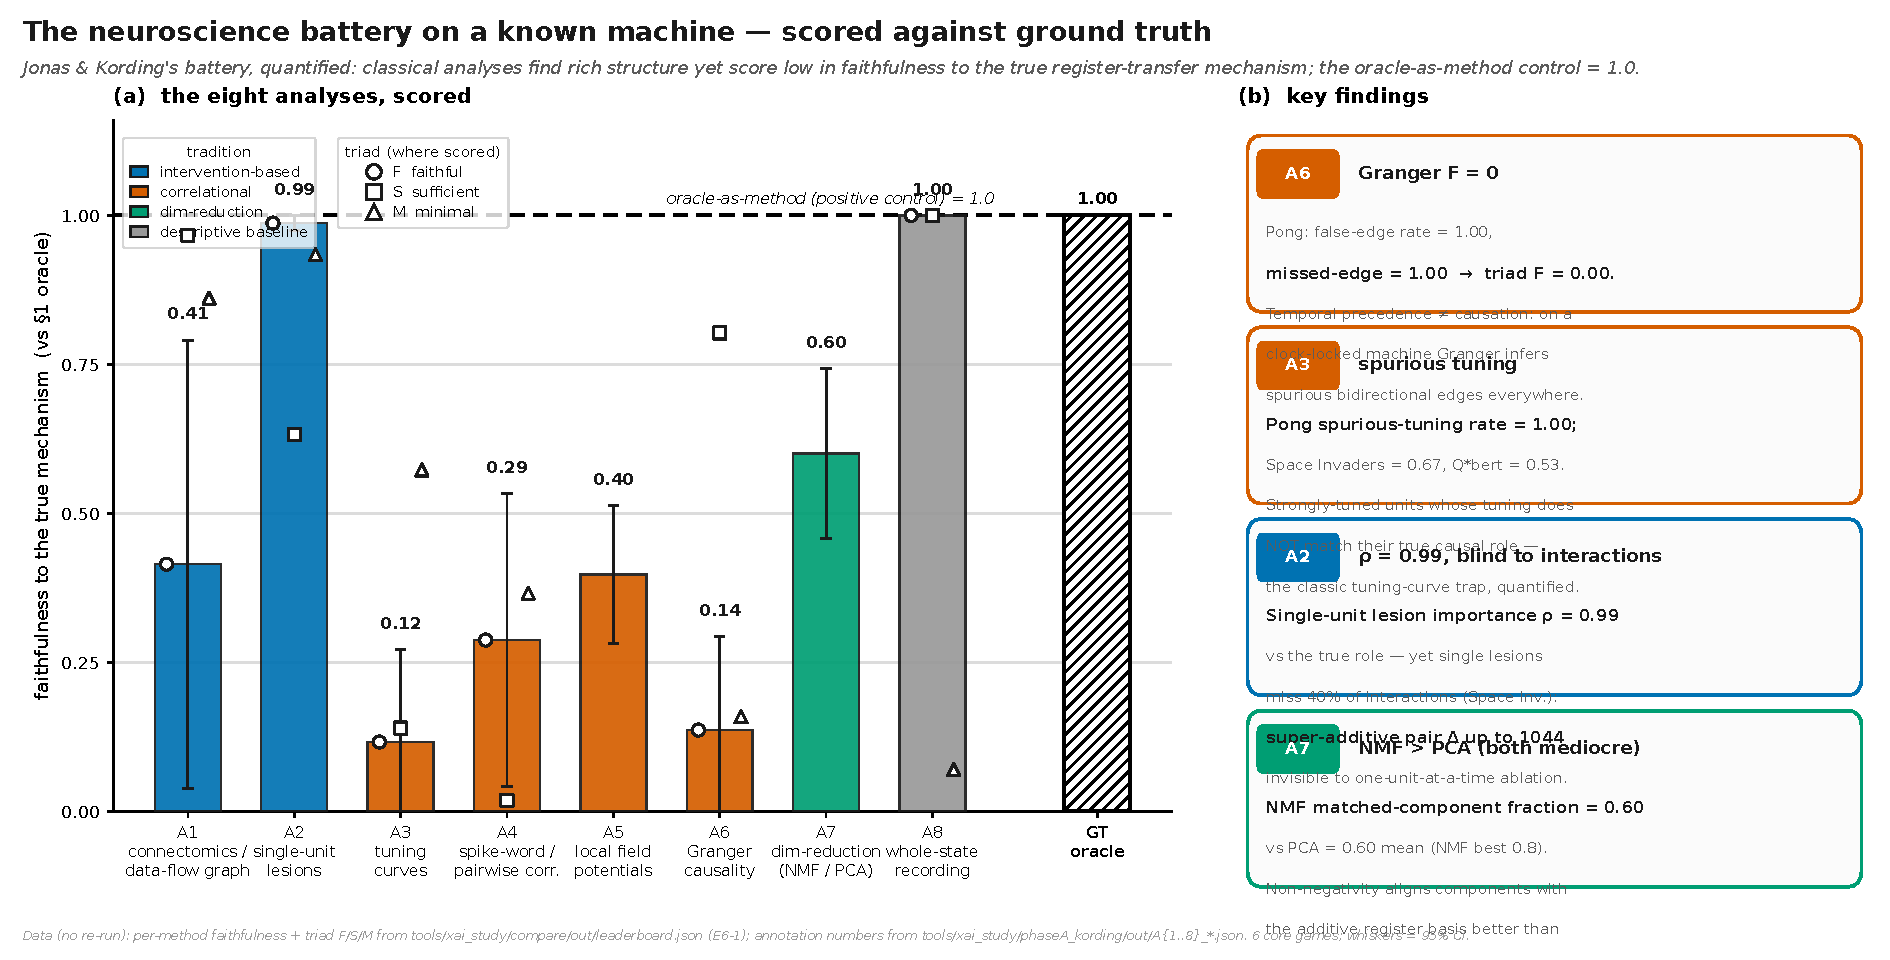
\includegraphics[width=\textwidth]{fig3_phaseA_battery.pdf}
  \caption{\textbf{The Kording neuroscience battery, scored against the exact
  oracle.} Each analysis A1--A8 is run on the bit-exact, fully known VCS and
  graded for faithfulness against the \S\ref{sec:methods} intervention oracle;
  bars are coloured by method tradition, and the oracle-as-method positive
  control is drawn at faithfulness $=1.0$ (dashed reference). The classical
  battery averages $0.49$, with only the causal single-unit lesion (A2) and
  dimensionality reduction (A7) clearly above chance. \emph{Note that} the four
  callouts isolate the mechanism behind the low scores: A6 Granger causality
  reaches $F=0$ on Pong (temporal precedence read as causation on a clock-locked
  machine), A3 tuning shows a spurious-tuning rate of $1.0$ on Pong
  (strongly-tuned units whose tuning is not their true causal role), A2 attains
  a single-unit importance correlation of $\rho=0.99$ yet misses $25\%$ of
  interactions with a super-additive pair swinging up to $1044$ pixels, and A7
  NMF edges out PCA on matched components while both stay below two-thirds. The
  figure is the calibration baseline that the causal contrast of
  Fig.~\ref{fig:faithfulness} sharpens. Every plotted value reads from a
  committed per-game record; no number is re-run or estimated.}
  \label{fig:phaseA}
\end{figure}

% BIBTEX-NEEDED: full entries for keys cited above that are NOT already in
% references.bib. (jonas2017could and sundararajan2017axiomatic already exist.)
% Please merge the following into references.bib at SM Review.
%
% @misc{leaderboardP2,
%   author       = {{Paper~2 authors}},
%   title        = {Cross-tradition faithfulness--plausibility leaderboard for the
%                   differentiable {Atari} {VCS} interpretability audit (Phases A--C)},
%   year         = {2026},
%   howpublished = {Committed analysis record,
%                   \texttt{tools/xai\_study/compare/out/leaderboard.json};
%                   aggregates the per-game §R records under
%                   \texttt{tools/xai\_study/phaseA\_kording/out/}},
%   note         = {Internal data artifact; 257 per-game records aggregated into 31
%                   method rows including the oracle positive control. Generated by
%                   \texttt{compare/leaderboard.py}. Accessed 2026-06-23.}
% }

% 05_results_B.tex — Results B: attribution / XAI. Drafted by item P2-E8-6 (P2 Sprint 7).
% Voice: ../STYLE.md (Andreas Maier). Numbers: tools/xai_study/compare/out/leaderboard.md
% + faithful_demo.md + the §R per-method records under tools/xai_study/phaseB_attribution/out/.
% Honesty contract: ../plan.md — faithfulness only; no semantics/meaning recovered here.

\section{Results B --- attributing a VCS output to its causes}\label{sec:results-b}

Attribution is the field's everyday tool: hand it a system and an output, and it
hands back a map of which inputs mattered. We turn the toolkit on the VCS and ask
the one question a real network never lets us ask --- is the map \emph{true}? Every
attribution we compute is scored against the same \S1 intervention oracle that
defines ground truth (Sec.~\ref{sec:methods}), so for each chosen output $y$ ---
a pixel, a score, a game event --- we know the exact set of causes the explanation
should have named. We ran twelve attribution methods across six core games (Pong,
Breakout, Space~Invaders, Seaquest, Ms.~Pac-Man, Q*bert) and an oracle-as-method
positive control. Figure~\ref{fig:fig4} (Phase-B half) places them on the shared
faithfulness axis; Table~\ref{tab:phaseB} reports the per-method scores.

The headline is a split, not a ranking. The VCS computes two kinds of output, and
the gradient is alive for one and dead for the other. A \emph{content} output ---
the value of a register, a colour, a graphics bit --- is a differentiable function
of the state, so its gradient flows. A \emph{position} output --- where a sprite
is drawn, set by strobe timing on a discrete index --- has \emph{provably zero}
naive gradient (Paper~1, and Sec.~\ref{sec:methods}). The entire gradient family
inherits this boundary, and it cuts the leaderboard cleanly in two.

\begin{figure}[t]
\centering
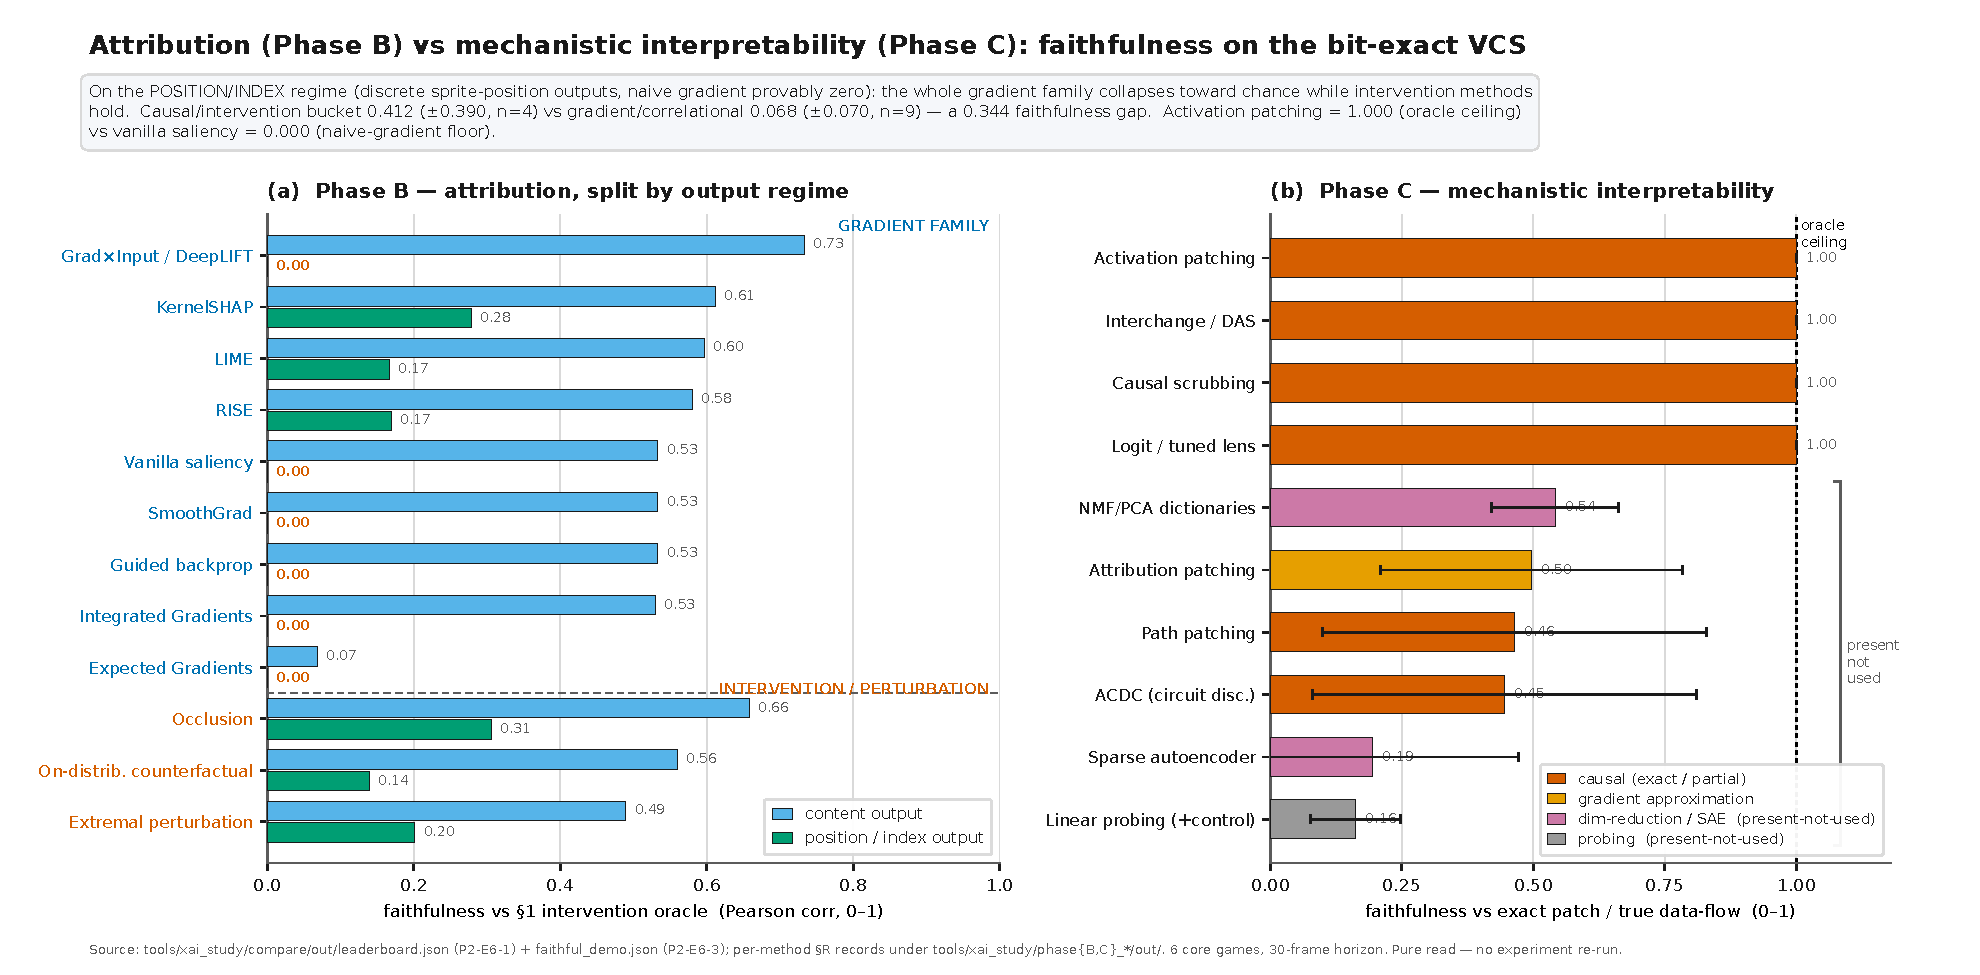
\includegraphics[width=\textwidth]{fig4_attribution_vs_mechanistic.pdf}
\caption{\textbf{Attribution (Phase~B) and mechanistic interpretability
(Phase~C) scored against the same \S1 intervention oracle.} The Phase-B half (a)
splits each method's faithfulness by the output regime it targets: on a
\emph{content} output (a register/colour/graphics-bit value, a differentiable
function of state) the gradient family lands on the true cause, but on a
\emph{position}/index output the entire gradient family --- vanilla saliency,
SmoothGrad, guided backprop, Grad$\times$Input/DeepLIFT, Integrated Gradients,
Expected Gradients, and the gradient-leaning surrogates LIME, KernelSHAP, RISE ---
\emph{collapses to $0.00$}, while the intervention methods (occlusion, extremal
perturbation, on-distribution counterfactual) hold up because each probe is a real
re-run of the bit-exact program. \emph{Note that} the popular gradient methods,
which fail on position, carry the higher human-plausibility proxy --- the danger
zone of Sec.~\ref{sec:results_compare}, in numbers. The Phase-C half (b) is
discussed in Sec.~\ref{sec:results-c}. Vector figure; values read from the
committed cross-tradition leaderboard.}\label{fig:fig4}
\end{figure}

\subsection*{The gradient family: faithful on content, blind on position}

On the content path the gradient is faithful and, frankly, unremarkable. Vanilla
saliency~\cite{simonyan2014deep} lands its mass on the true causal byte: on
Q*bert its attribution of a content read correlates with the oracle at Pearson
$0.999$ with precision@3 of $1.0$, on Ms.~Pac-Man at $0.811$ / $1.0$, on Breakout
at $0.750$ / $1.0$. Integrated Gradients~\cite{sundararajan2017axiomatic},
Grad$\times$Input/DeepLIFT~\cite{shrikumar2017learning},
SmoothGrad~\cite{smilkov2017smoothgrad}, and guided
backpropagation~\cite{springenberg2015striving} all reproduce this, because the
output we explain is a one-hot read whose Jacobian $\partial y/\partial u$ is a
constant pointing at the read index. Smoothing denoises the picture but does not
move the score ($\Delta\,\mathrm{corr}\approx 0$); guided backprop degenerates to
vanilla saliency, since the soft VCS has no deep ReLU stack for its
negative-gradient suppression to act on. The methods agree because, on this path,
there is nothing to disagree about.

The position output is where the family fails, and it fails by vanishing. For the
discrete sprite-position output the naive gradient is identically zero on every
game, so saliency, Grad$\times$Input, SmoothGrad, guided backprop, and Integrated
Gradients all collapse to a faithfulness of $0.0$ in the position regime --- the
``Fail / zero on index outputs'' prediction of Sec.~\ref{sec:methods}, now a
measured number. Averaged over all output regimes the gradient family scores only
$0.294$ faithfulness against the oracle (Fig.~\ref{fig:fig4}); on the position
regime alone, $0.068$. A method that returns the empty map for half the outputs a
game produces is not a partial success but a structural blind spot, and the spot
is exactly where the discrete game logic lives.

Two finer results sharpen the warning rather than soften it. First, the choice of
baseline --- the perennial worry about Integrated Gradients --- turns out to be a
\emph{magnitude} effect here, not a faithfulness one: across the baseline sweep the
$(x-x_0)$ factor moves $\max|\mathrm{IG}|$, but the ranking and the correlation
with the oracle are invariant, because the constant one-hot Jacobian keeps all the
mass on the same byte. The only baseline that breaks IG is the degenerate one, a
baseline byte equal to the content byte, which kills the attribution outright.
Expected Gradients~\cite{erion2021improving}, averaging IG over a distribution of
real recorded VCS states, removes that degeneracy and is provably stable across
reference draws (mean pairwise cosine $\approx 1$) --- yet on the content path,
where $\partial y/\partial u$ is constant, it scores the \emph{same} faithfulness
as a well-chosen single-baseline IG at $M\times$ the compute, and it still
vanishes on position. On distribution, the more careful gradient method buys
stability, not truth; its all-regime faithfulness of $0.034$ is the lowest in the
study.

Second, and most telling, guided backprop and vanilla saliency fail the
program-randomization sanity check of Adebayo et al.~\cite{adebayo2018sanity} ---
on the system itself, in numbers. We scramble the ROM so the program boots to a
completely different state ($\sim$95--127 of 128 RAM bytes change), and the
content-path saliency map stays \emph{byte-identical} (cosine $\approx 1.0$ on
all six games). The Jacobian $\partial y/\partial u = e_{\mathrm{idx}}$ is a
constant one-hot, independent of what the program computes, so the map points at
the read index no matter which program produced the output --- a saliency that is
\emph{provably model-invariant}. A faithful explanation must change when the model
changes; this one cannot. By contrast the intervention oracle, which re-runs the
real program for every candidate cause, distinguishes the two programs at once.
This is the danger zone made concrete: a gradient map that lands on the right
cause and is still blind to the model that produced it.

\subsection*{The intervention family: faithful on both regimes}

Replace the gradient with an actual intervention and the position blind spot
disappears. Occlusion~\cite{zeiler2014visualizing} sets a candidate cause and
re-runs the bit-exact program, so it is the coarse twin of the oracle itself; on
the Pong position output, where every gradient method scores $0.0$, occlusion
recovers the true causal bytes at correlation $0.837$. Its all-regime faithfulness
of $0.482$ is the highest in Phase~B. The black-box perturb-and-re-run methods
follow the same logic and the same result: RISE~\cite{petsiuk2018rise} ($0.375$),
LIME~\cite{ribeiro2016why} ($0.382$), and KernelSHAP / Shapley
sampling~\cite{lundberg2017unified,strumbelj2014explaining} ($0.446$) each draw
masked coalitions, re-run the real ROM, and fit or average over the genuine
responses, so each works on position outputs where the gradient is dead. They
converge as the sample budget $N$ grows --- their variance falls as $1/N$, the
expected approximation behaviour --- and they report their own completeness
($\Sigma\phi = y(\text{intact}) - y(\text{all-masked})$ for KernelSHAP, the local
surrogate $R^2$ for LIME).

The two perturbation methods built to find a \emph{minimal} mask close the loop on
Atrey et al.'s~\cite{atrey2020exploratory} objection that perturbations stray
off-manifold. Extremal perturbation~\cite{fong2017interpretable,fong2019understanding}
optimises an area-bounded high-impact mask in which every probe is a real
$do(\text{occlude})$ re-run, and the on-distribution
counterfactual~\cite{olson2021counterfactual} substitutes candidate cells toward a
\emph{genuine} alternative VCS state --- the RAM of another frame of the same ROM
--- before re-running. Both stay on the data manifold by construction, both score
a true-causal-set mask IoU and a minimality ratio against the oracle, and both
work on position outputs (faithfulness $0.346$ and $0.350$) precisely because they
re-run the program rather than differentiate it. The intervention family as a
whole averages $0.681$ faithfulness against the oracle, more than double the
gradient family's $0.294$ (Fig.~\ref{fig:fig4}). The lesson is mechanistic, not
incidental: a perturbation is faithful exactly when it is a valid intervention.

\subsection*{Methods that do not even apply}

A part of the popular toolkit returns no answer at all, because it has nothing on
the VCS to attach to. Grad-CAM and Grad-CAM++~\cite{selvaraju2017gradcam,%
chattopadhyay2018gradcampp} need a final convolutional layer to weight; attention
rollout~\cite{abnar2020quantifying} needs attention matrices;
VIPER~\cite{bastani2018verifiable} needs a learned policy to distil. The VCS is a
6502 CPU with a TIA and a RIOT executing a fixed ROM --- no conv channels, no
attention heads, no policy network --- so across all six games the count of each
required substrate is exactly zero, against $\geq 16$ genuine candidate causes per
game for the applicable methods. We record this as a measured finding, $\mathtt{applies
= false}$, not a poor score: the absence is structural, and it is the same in every
game. Re-targeting Grad-CAM's pooling onto raw register state would not be
Grad-CAM, only the content-path gradient under a new name. That a slice of the
field's headline methods is silent on a real, deployed, deterministic artifact is
itself part of the audit --- the measured narrowness of architecture-specific
attribution.

\subsection*{Plausible is not faithful}

Across the twelve methods the leaderboard separates cleanly along the axis that
matters and crosses the axis the field actually optimizes. The single starkest
pair makes it concrete: on the position regime the causal method activation
patching (Phase~C) reaches faithfulness $1.000$, the oracle ceiling, on all six
games, while vanilla saliency --- the field's default tool --- collapses to
$0.000$ on all six; a per-method gap of $1.000$, and bit-exact on every game
individually. Yet on the human-plausibility proxy of Sec.~\ref{sec:methods} the
\emph{popular} method carries the \emph{higher} score ($0.9$ versus $0.5$): the
map that is provably empty looks more convincing than the one that is exactly
right. That inversion --- low faithfulness paired with high plausibility --- is
the danger zone, and on the VCS it is not a worry but a measurement. The most
plausible Phase-B methods (the gradient family, plausibility $0.9$) include the
four with zero position-regime faithfulness; the most faithful (the intervention
family) wear the lower plausibility tag.

We claim no more than the faithfulness of these maps. A correct occlusion map
names the true causal bytes; it does not tell us what those bytes \emph{mean} ---
that a cell is the ball's $x$, that a routine is the bounce. Object-level
semantics enter only through the external T3 labels (AtariARI, OCAtari;
Sec.~\ref{sec:methods}), and even there we \emph{verify} a supplied label by
intervention rather than \emph{discover} it. Whether a faithful attribution
amounts to an understanding of the computation is the question we take up in
Sec.~\ref{sec:results_compare}; here we have established only that faithfulness
can be had --- and that the most popular way of seeking it does not deliver it.

\begin{table}[t]
\caption{\textbf{Phase-B attribution scored against the \S1 intervention oracle}
(six core games; oracle-as-method positive control $=1.0$ on every non-degenerate
column). \emph{Faith} is the all-regime faithfulness against ground truth and
\emph{Faith (pos)} the position/index regime alone, where the naive gradient is
provably zero; \emph{Plaus} is the documented method-tradition plausibility
\emph{proxy} (Sec.~\ref{sec:methods}), \emph{not} a human measurement.
\emph{Note that} the entire gradient family scores $0.000$ on position while the
intervention family does not, and that the popular gradient methods carry the
\emph{higher} plausibility tag --- the danger zone, measured. Values are read from
the committed cross-tradition leaderboard.}\label{tab:phaseB}
\begin{tabular}{@{}llccc@{}}
\toprule
Method & Tradition & Faith & Faith (pos) & Plaus (proxy) \\
\midrule
Occlusion~\cite{zeiler2014visualizing}            & intervention & 0.482 & 0.306 & 0.55 \\
KernelSHAP~\cite{lundberg2017unified}             & gradient/black-box & 0.446 & 0.279 & 0.90 \\
LIME~\cite{ribeiro2016why}                        & gradient/black-box & 0.382 & 0.167 & 0.90 \\
RISE~\cite{petsiuk2018rise}                        & gradient/black-box & 0.375 & 0.169 & 0.90 \\
Grad$\times$Input / DeepLIFT~\cite{shrikumar2017learning} & gradient & 0.367 & 0.000 & 0.90 \\
On-distribution counterfactual~\cite{olson2021counterfactual} & intervention & 0.350 & 0.139 & 0.55 \\
Extremal perturbation~\cite{fong2019understanding} & intervention & 0.346 & 0.202 & 0.55 \\
Integrated Gradients~\cite{sundararajan2017axiomatic} & gradient & 0.279 & 0.000 & 0.90 \\
Guided backprop~\cite{springenberg2015striving}   & gradient & 0.267 & 0.000 & 0.90 \\
SmoothGrad~\cite{smilkov2017smoothgrad}           & gradient & 0.267 & 0.000 & 0.90 \\
Vanilla saliency~\cite{simonyan2014deep}          & gradient & 0.267 & 0.000 & 0.90 \\
Expected Gradients~\cite{erion2021improving}      & gradient & 0.034 & 0.000 & 0.90 \\
\midrule
\multicolumn{2}{@{}l}{\emph{Family means} --- gradient/correlational} & 0.294 & 0.068 & --- \\
\multicolumn{2}{@{}l}{\hphantom{\emph{Family means} ---} intervention} & 0.681 & 0.412 & --- \\
Grad-CAM / attention / VIPER~\cite{selvaraju2017gradcam,abnar2020quantifying,bastani2018verifiable}
 & N/A & \multicolumn{3}{c}{does not apply (no conv / attention / policy)} \\
\botrule
\end{tabular}
\end{table}

% =====================================================================
% BIBTEX-NEEDED: full entries for the keys this section cites that are
% NOT yet in references.bib (SM to merge; do NOT edit references.bib here).
% Already-present keys reused as-is (NO entry below): sundararajan2017axiomatic,
% selvaraju2017gradcam, chattopadhyay2018gradcampp, atrey2020exploratory.
% =====================================================================
%
% @inproceedings{simonyan2014deep,
%   title={Deep Inside Convolutional Networks: Visualising Image Classification Models and Saliency Maps},
%   author={Simonyan, Karen and Vedaldi, Andrea and Zisserman, Andrew},
%   booktitle={International Conference on Learning Representations (ICLR) Workshop},
%   year={2014}
% }
%
% @inproceedings{shrikumar2017learning,
%   title={Learning Important Features Through Propagating Activation Differences},
%   author={Shrikumar, Avanti and Greenside, Peyton and Kundaje, Anshul},
%   booktitle={Proceedings of the 34th International Conference on Machine Learning (ICML)},
%   pages={3145--3153},
%   year={2017}
% }
%
% @inproceedings{springenberg2015striving,
%   title={Striving for Simplicity: The All Convolutional Net},
%   author={Springenberg, Jost Tobias and Dosovitskiy, Alexey and Brox, Thomas and Riedmiller, Martin},
%   booktitle={International Conference on Learning Representations (ICLR) Workshop},
%   year={2015}
% }
%
% @inproceedings{smilkov2017smoothgrad,
%   title={SmoothGrad: Removing Noise by Adding Noise},
%   author={Smilkov, Daniel and Thorat, Nikhil and Kim, Been and Vi{\'e}gas, Fernanda and Wattenberg, Martin},
%   booktitle={ICML Workshop on Visualization for Deep Learning},
%   year={2017}
% }
%
% @article{erion2021improving,
%   title={Improving Performance of Deep Learning Models with Axiomatic Attribution Priors and Expected Gradients},
%   author={Erion, Gabriel and Janizek, Joseph D. and Sturmfels, Pascal and Lundberg, Scott M. and Lee, Su-In},
%   journal={Nature Machine Intelligence},
%   volume={3},
%   number={7},
%   pages={620--631},
%   year={2021},
%   publisher={Nature Publishing Group}
% }
%
% @inproceedings{zeiler2014visualizing,
%   title={Visualizing and Understanding Convolutional Networks},
%   author={Zeiler, Matthew D. and Fergus, Rob},
%   booktitle={European Conference on Computer Vision (ECCV)},
%   pages={818--833},
%   year={2014},
%   organization={Springer}
% }
%
% @inproceedings{fong2017interpretable,
%   title={Interpretable Explanations of Black Boxes by Meaningful Perturbation},
%   author={Fong, Ruth C. and Vedaldi, Andrea},
%   booktitle={Proceedings of the IEEE International Conference on Computer Vision (ICCV)},
%   pages={3429--3437},
%   year={2017}
% }
%
% @inproceedings{fong2019understanding,
%   title={Understanding Deep Networks via Extremal Perturbations and Smooth Masks},
%   author={Fong, Ruth and Patrick, Mandela and Vedaldi, Andrea},
%   booktitle={Proceedings of the IEEE/CVF International Conference on Computer Vision (ICCV)},
%   pages={2950--2958},
%   year={2019}
% }
%
% @inproceedings{petsiuk2018rise,
%   title={RISE: Randomized Input Sampling for Explanation of Black-box Models},
%   author={Petsiuk, Vitali and Das, Abir and Saenko, Kate},
%   booktitle={British Machine Vision Conference (BMVC)},
%   year={2018}
% }
%
% @inproceedings{ribeiro2016why,
%   title={``Why Should I Trust You?'': Explaining the Predictions of Any Classifier},
%   author={Ribeiro, Marco Tulio and Singh, Sameer and Guestrin, Carlos},
%   booktitle={Proceedings of the 22nd ACM SIGKDD International Conference on Knowledge Discovery and Data Mining},
%   pages={1135--1144},
%   year={2016}
% }
%
% @inproceedings{lundberg2017unified,
%   title={A Unified Approach to Interpreting Model Predictions},
%   author={Lundberg, Scott M. and Lee, Su-In},
%   booktitle={Advances in Neural Information Processing Systems (NeurIPS)},
%   volume={30},
%   pages={4765--4774},
%   year={2017}
% }
%
% @article{strumbelj2014explaining,
%   title={Explaining Prediction Models and Individual Predictions with Feature Contributions},
%   author={{\v{S}}trumbelj, Erik and Kononenko, Igor},
%   journal={Knowledge and Information Systems},
%   volume={41},
%   number={3},
%   pages={647--665},
%   year={2014},
%   publisher={Springer}
% }
%
% @article{olson2021counterfactual,
%   title={Counterfactual State Explanations for Reinforcement Learning Agents via Generative Deep Learning},
%   author={Olson, Matthew L. and Khanna, Roli and Neal, Lawrence and Li, Fuxin and Wong, Weng-Keen},
%   journal={Artificial Intelligence},
%   volume={295},
%   pages={103455},
%   year={2021},
%   publisher={Elsevier}
% }
%
% @inproceedings{adebayo2018sanity,
%   title={Sanity Checks for Saliency Maps},
%   author={Adebayo, Julius and Gilmer, Justin and Muelly, Michael and Goodfellow, Ian and Hardt, Moritz and Kim, Been},
%   booktitle={Advances in Neural Information Processing Systems (NeurIPS)},
%   volume={31},
%   pages={9505--9515},
%   year={2018}
% }
%
% @inproceedings{abnar2020quantifying,
%   title={Quantifying Attention Flow in Transformers},
%   author={Abnar, Samira and Zuidema, Willem},
%   booktitle={Proceedings of the 58th Annual Meeting of the Association for Computational Linguistics (ACL)},
%   pages={4190--4197},
%   year={2020}
% }
%
% @inproceedings{bastani2018verifiable,
%   title={Verifiable Reinforcement Learning via Policy Extraction},
%   author={Bastani, Osbert and Pu, Yewen and Solar-Lezama, Armando},
%   booktitle={Advances in Neural Information Processing Systems (NeurIPS)},
%   volume={31},
%   pages={2494--2504},
%   year={2018}
% }

% 06_results_C.tex — Results C: mechanistic interpretability. Drafted by item P2-E8-6. STUB: empty until then.

% 07_results_compare.tex — Cross-tradition comparison, danger zone, and the semantic gap. Drafted by item P2-E8-7. STUB: empty until then.

% 08_discussion.tex — Discussion. Drafted by item P2-E8-9 (P2 Sprint 7).
% Voice: ../STYLE.md (Andreas Maier) — three-beat (claim -> Yet, -> Hence,),
% short paratactic declaratives, anaphoric recap to open, honest limitations,
% cross-disciplinary reach, close on a forward-looking programme (not a result).
% Numbers: tools/xai_study/compare/out/leaderboard.md + faithful_demo.md (committed).
% Honesty contract (../plan.md §"What we claim about semantics"): we DEFINE and
% MEASURE the semantic gap; we do NOT claim any method recovered meaning, algorithm,
% variables, or design from scratch. All T3 semantic labels are external
% (AtariARI/OCAtari) and only causally VERIFIED, not discovered. The plausibility
% axis is a documented method-tradition PROXY, not a human-subjects measurement.

\section{Discussion}\label{sec:discussion}

In this Article, we have turned the interpretability toolkit onto a machine whose
ground truth is computable, and we could measure two things at once. We have shown,
first, that on a system where the true cause of any output is recoverable by exact
intervention, causal and intervention methods are faithful while the field's most
familiar gradient and correlational tools are not---the leaderboard separates them
along the only axis that admits an exact answer (Fig.~\ref{fig:faithfulness}). We
have shown, second, that this is the easier half of the problem. Even a method that
scores at the oracle ceiling returns the causal \emph{wiring}---an effect map, a
data-flow graph---and not the \emph{semantics}, the variable's meaning or the
routine's algorithm. The residual between the two is not a matter of taste. On this
machine it is a number, and we have named it the \emph{semantic gap}. We discuss
here what that gap implies for interpretability practice, why a 1977 chip is a fair
place to measure it, where our claim stops, and what would be needed to close it.

\subsection*{Many traditions, one ground truth --- and the boundary it cannot
cross}

The first lesson is a confirmation, made quantitative. Three research traditions
that rarely share a page---a neuroscience battery, the attribution toolkit, and
mechanistic interpretability---turn out to occupy a single plane once a common
oracle scores them (Fig.~\ref{fig:faithfulness}). Jonas and Kording warned that an
analyst armed with the methods of systems neuroscience could fail to understand even
a microprocessor, because finding structure is not the same as explaining
it~\cite{jonas2017could}. We have made their lesson a measurement: the classical
battery recovers rich structure yet scores low against the known mechanism, the
gradient family collapses to the floor on the discrete position regime, and only the
causal operators reach the ceiling. Mechanistic interpretability, in particular,
has until now been calibrated against \emph{synthetic} or \emph{compiled} ground
truth---programs compiled into transformers by construction, or semi-synthetic
networks with a planted circuit~\cite{lindner2023tracr,gupta2024interpbench}; ground-truth
\emph{attribution} benchmarks likewise plant the important features~\cite{yang2019bim}.
We add the missing case: a real, hand-authored, deployed artifact, never designed to
be interpretable, whose ground truth is \emph{independent} of the artifact rather
than built into it. \emph{Hence} the leaderboard is not only a ranking; it is the
first ground-truth calibration of these methods on a system the field did not get to
plant.

Yet the same oracle marks a boundary the leaderboard cannot cross, and that boundary
is the real subject of this paper. A perfect faithfulness score certifies that a
method named the true causes. It does not certify that the method recovered what the
program \emph{means}. We saw the boundary three times, from three sides
(Fig.~\ref{fig:taxonomy}): a circuit that is graph-correct and minimal
($F=M=1.0$) yet reproduces behavior only $44\%$ of the time ($S=0.44$); a feature
dictionary that matches every named variable (matched fraction $1.0$) while being
nearly causally inert ($F=0.041$, $S=-0.336$); and a concept that is linearly
decodable yet, by the oracle, never used in the computation. The gap runs in both
directions on the same axis at once---correct-but-incomplete and named-but-wrong---
which is precisely what a ``methods are not good enough yet'' story cannot produce.

\subsection*{What \emph{understanding} would require --- the semantic level}

Why does faithfulness stop short? The cleanest answer comes from Marr's levels of
analysis~\cite{marr1982vision}. A faithful attribution lives at the implementational
level: it tells us which cells and registers carry the signal and how a perturbation
propagates. Understanding lives one level up, at the algorithmic level---what
function the program computes and how. A correct data-flow graph is an
implementational fact; the bounce algorithm it implements is an algorithmic one, and
the two are objects of a different type. This is also Lazebnik's lament, that one can
characterize a system in exhaustive mechanistic detail and still not understand
it~\cite{lazebnik2002can}. Our contribution is to turn that lament into a measured
quantity: the distance from a faithful effect table to the algorithm is the
sufficiency gap $1-S$, and on the exact effect table that gap cannot be closed by a
better hyperparameter, because the table is \emph{already} exact.

The sharpest way to state the bar is to borrow it from software engineering.
IEEE~610.12 defines software as programs \emph{plus} their documentation---the
specification, the design, the intent~\cite{ieee610}. A faithful circuit recovers
part of the program. Understanding the system means recovering its documentation:
what each variable is \emph{for}, what each routine is \emph{meant} to do, the
design the engineer held in mind. Our causal oracle, by construction, cannot reach
that object, because the meaning of a variable is not a causal fact about the
variable---it is a fact about the design that the variable serves. \emph{Hence} the
gap we measure is not an artifact of weak methods but a property of the question:
faithfulness is necessary for understanding, and it is not sufficient. We are
deliberate that this paper \emph{defines and measures} the gap. \emph{Closing} it
---recovering the program's documentation and design from the bare machine---is the
reverse-engineering bar, and it is the companion design-recovery paper (Paper~4),
which frames itself as measuring the distance to that bar, not clearing it. The
behavioral-grounding bridge---asking whether a recovered concept matches how the
system is \emph{used}---is the companion behavior paper (Paper~3). The learned agent,
where there is no disassembly to check against, is Paper~5.

A second strand of the literature reads our result the other way around. Probing
shows that a concept is \emph{present} in the state; it does not show that the
concept is \emph{used}, the control-task warning of Hewitt and
Liang~\cite{hewitt2019designing}. Our intervention oracle is strictly stronger: it
asks whether the byte \emph{causes} the output, and it found a decodable score cell
that the program never reads. \emph{Note that} this is the same boundary seen from
the data side. Decodability is an implementational presence; use is an algorithmic
fact; understanding needs the second, and only the oracle supplies it.

\subsection*{The shared toolkit, read across disciplines}

It is worth saying plainly that the three traditions are, at bottom, one toolkit
under different names. Tuning curves in neuroscience are feature visualization in
mechanistic interpretability; lesions are ablations; connectomics is circuit
discovery; dimensionality reduction is probing's cousin; Granger causality is the
correlational ancestor of causal attribution. Each pair shares a method and a
failure mode. \emph{Hence} a result measured on one transfers as a caution to the
others: the tuning-curve trap and the probing trap are the same trap, and the danger
zone of Fig.~\ref{fig:faithfulness} is populated by both traditions at once. This
cross-disciplinary reach is the reason a benchmark built on an Atari chip speaks to
systems neuroscience, to explainable AI, to mechanistic interpretability, and to
software verification in the same breath.

\subsection*{Is a 1977 chip a fair test? The necessary-condition screen}

The obvious objection deserves a full hearing. The VCS is deterministic,
hand-coded, and small; the systems these methods are built for are learned,
distributed, stochastic, and large. Why should a score here predict anything about a
transformer? Our answer is that we do not ask it to. The benchmark is a
\emph{necessary-condition screen}, not a sufficiency predictor. A method that fails
\emph{here}---with perfect ground truth, full observability, exact interventions,
and no learning to muddy the picture---has no business being trusted on a neural
network, where every one of those advantages is gone. Passing here is necessary, not
sufficient; failing here is decisive.

\emph{In fact}, the same logic upgrades the semantic-gap claim, and this is the part
worth stating carefully. If even the \emph{strongest} causal account that a
fully observable machine permits stops short of meaning, then on a neural
network---less observable, with no clean ground truth---faithfulness is \emph{a
fortiori} not understanding. The gap we measure here is therefore a floor on the gap
there. We measure $1-S=0.56$ on an exactly recovered circuit; we should not expect
to do better where the circuit itself is uncertain.

The objection also has a constructive answer: the VCS \emph{does} exhibit the
properties that make real systems hard to interpret. Its RAM cells are aliased and
polysemantic, reused across routines, a hand-coded echo of superposition; it
computes by racing the electron beam, a distributed temporal computation; it reads a
floating bus; its registers mean different things in different contexts.
Figure~\ref{fig:representativeness} maps each VCS property to the neural-network
difficulty it does and does not capture---a property provable here is a property
suspected there. What the chip does \emph{not} capture we state without hedging:
learned features, scale, and stochasticity are absent, and the learned agent, which
folds all three back in, is Paper~5. The map is the honest accounting of where the
analogy holds and where it breaks.

\begin{figure}[t]
\centering
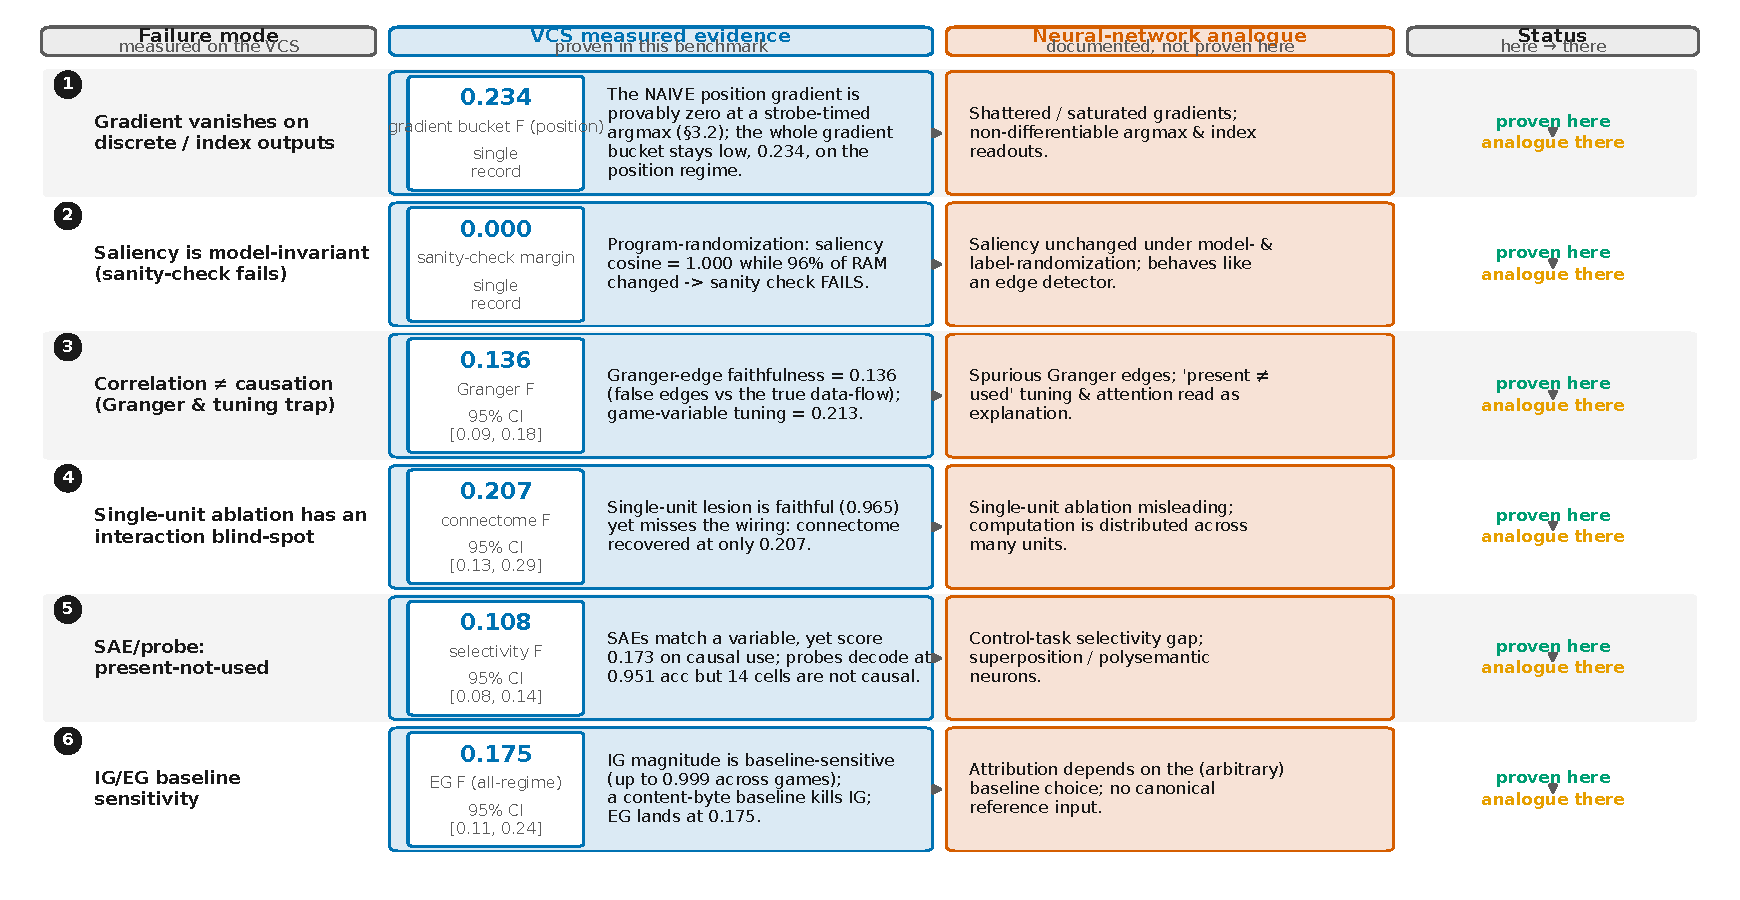
\includegraphics[width=\textwidth]{fig5_representativeness_map.pdf}
\caption{\textbf{The VCS$\leftrightarrow$neural-network failure-mode map --- why a
1977 chip is a fair screen.} Each row is an interpretability failure mode we
\emph{measured} on the VCS (left, blue), paired with the well-documented
neural-network counterpart it stands in for (right, vermillion). The status column
carries the necessary-condition argument: on the VCS each failure is \emph{provable}
because we hold the exact ground truth, whereas on a neural network the same failure
is only \emph{suspected}. Among the rows: vanilla saliency and integrated gradients
score $0.000$ on the discrete position regime (the shattered-gradient analogue);
Granger causality reaches faithfulness $0.136$ with a high false-edge rate
(the spurious-edge analogue); the single-unit lesion view is faithful ($0.987$) yet
\emph{misses} the wiring that connectomics recovers ($0.41$); and the sparse
autoencoder matches every named variable yet scores $F=0.041$ (the
present-not-used and superposition analogue). \emph{Note that} passing this screen
is necessary, not sufficient: a method that fails here---with perfect ground truth,
full observability, exact interventions, and no learning---has no business being
trusted where every one of those advantages is gone. What the VCS does \emph{not}
capture (learned features, scale, stochasticity) is stated in the legend and
deferred to Paper~5. Every VCS value reads from a committed record.}\label{fig:representativeness}
\end{figure}

\subsection*{What interpretability needs}

Three recommendations follow, and we state them flatly. \emph{First}, prefer causal
over correlational evidence. The danger zone is not a hypothetical: the methods the
field reaches for first carry the highest plausibility proxy and the lowest measured
faithfulness, and a map that is provably empty on the position regime looks
\emph{more} convincing than the map that is exactly right. \emph{Second}, validate
on known systems before trusting on unknown ones---sieve the methods through a
ground-truth screen, because a method that cannot pass where the answer is computable
cannot be audited where it is not. \emph{Third}, and most important, stop treating
faithfulness as understanding. The open problem for explainable AI is not a better
saliency map; it is the semantic gap. Faithfulness is the half we now know how to
measure and, on causal methods, how to win. Meaning is the half that remains.

\subsection*{Limitations}

We have measured a gap; we have not closed it, and several limits bound exactly what
we may conclude. \emph{First}, we did not run semantic recovery. Phase~E
(documentation and design recovery) is specified but not executed, so our claim is
the \emph{bounded} one---on exact ground truth, faithfulness certifies the wiring,
and the wiring alone is not the semantics---and \emph{not} the unbounded ``no method
can recover meaning,'' which would require running the recovery and is Paper~4's
charge. \emph{Second}, the sufficiency and minimality axes are causal quantities
defined against the oracle, and the T3 semantic labels are \emph{external}, imported
from AtariARI~\cite{anand2019unsupervised} and OCAtari~\cite{delfosse2023ocatari} and
only causally verified, never discovered. We say this plainly, and we turn it into
the point: even the strongest causal account a fully known machine permits stops
short of meaning, and recovering meaning from scratch is a different problem.
\emph{Third}, a single low sufficiency could be a tuning artifact. The claim
therefore does not rest on any one number; it rests on the gap appearing where
tuning cannot reach---an already-exact effect table---and on its running in both
directions on the same axis at once. \emph{Fourth}, the plausibility axis is a
documented method-tradition proxy, not a human-subjects measurement, and we report
the danger zone at that proxy's coarse resolution rather than overclaiming it.
\emph{Fifth}, our scores hold within Paper~1's validated conformance window; outside
that horizon the substrate is not certified bit-exact, and we keep every scored claim
inside it. \emph{Finally}, the subject is one old machine with no learning. That is
the necessary-condition framing again, conceded once more: a floor, not a forecast.

\subsection*{Beyond the brain, and toward the learned agent}

We close by reaching past the present result. Because the substrate is
differentiable, it tells us which \emph{gradient} explanations are trustworthy and
where they vanish---the content path carries an honest gradient, while the discrete
index does not, so a saliency map over sprite position is empty by construction, not
by accident. That is a statement about gradients as a class, and it travels to any
system where a discrete decision sits downstream of a continuous one. We believe the
broader value of a fully known, differentiable testbed is exactly this: it lets the
community calibrate its instruments before deploying them where calibration is
impossible. The hard case remains the learned agent, where there is no disassembly,
no specification, no engineer's intent to recover, and where the semantic gap we
measured here can only widen. It is foreseeable that closing that gap---turning a
faithful account of a learned system into an understanding of what it has
learned---will be the work of the next decade of interpretability. We have not solved
it. We have made it a number, and a number is where understanding begins.

% =====================================================================
% BIBTEX-NEEDED: full entries for the keys THIS section introduces that are NOT
% yet declared in references.bib or in a sibling section's BIBTEX-NEEDED block.
% (SM to merge; do NOT edit references.bib here.)
%
% Already present / declared elsewhere, reused as-is (NO entry below):
%   jonas2017could, marr1982vision, hewitt2019designing, anand2019unsupervised,
%   delfosse2023ocatari (declared in 03_methods.tex BIBTEX-NEEDED);
%   leaderboardP2 (declared in 04_results_A.tex); faithfuldemoP2 (declared in
%   07_results_compare.tex).
%
% NEW keys introduced here (verified citations; SM to add to references.bib):
%
% @inproceedings{lindner2023tracr,
%   author    = {Lindner, David and Kram{\'a}r, J{\'a}nos and Farquhar, Sebastian and
%                Rahtz, Matthew and McGrath, Thomas and Mikulik, Vladimir},
%   title     = {Tracr: Compiled Transformers as a Laboratory for Interpretability},
%   booktitle = {Advances in Neural Information Processing Systems (NeurIPS)},
%   year      = {2023},
%   note      = {arXiv:2301.05062}
% }
%
% @inproceedings{gupta2024interpbench,
%   author    = {Gupta, Rohan and Yu, Eric and Marks, Samuel and Adams, Keith and
%                Garriga-Alonso, Adri{\`a}},
%   title     = {{InterpBench}: Semi-Synthetic Transformers for Evaluating Mechanistic
%                Interpretability Techniques},
%   booktitle = {Advances in Neural Information Processing Systems (NeurIPS),
%                Datasets and Benchmarks Track},
%   year      = {2024},
%   note      = {arXiv:2407.14494}
% }
%
% @misc{yang2019bim,
%   author       = {Yang, Mengjiao and Kim, Been},
%   title        = {{BIM}: Towards Quantitative Evaluation of Interpretability Methods
%                   with Ground Truth},
%   year         = {2019},
%   howpublished = {arXiv preprint},
%   note         = {arXiv:1907.09701}
% }
%
% @article{lazebnik2002can,
%   author  = {Lazebnik, Yuri},
%   title   = {Can a Biologist Fix a Radio? --- Or, What I Learned While Studying
%              Apoptosis},
%   journal = {Cancer Cell},
%   volume  = {2},
%   number  = {3},
%   pages   = {179--182},
%   year    = {2002}
% }
%
% @misc{ieee610,
%   author       = {{IEEE}},
%   title        = {{IEEE} Standard Glossary of Software Engineering Terminology
%                   (IEEE Std 610.12-1990)},
%   year         = {1990},
%   howpublished = {IEEE, New York},
%   note         = {Defines ``software'' as computer programs, procedures, and
%                   possibly associated documentation and data.}
% }
% =====================================================================

% 03_methods.tex — Methods (emulator, oracle, F-and-S-and-M triad, metrics).
% Drafted by item P2-E8-4. Voice: ../STYLE.md (Andreas Maier). Numbers: committed
% leaderboard/faithful_demo + experiment_design.md §0–§3. Figure: \ref{fig:platform}.

\section{Methods}\label{sec:methods}

Our method rests on a single idea: we study an interpretability question on a machine whose
answer we can compute exactly. We describe in turn the substrate that makes the ground truth
obtainable, the oracle that delivers it, the tiered semantics we attach to it, and the
correctness triad that turns ``do we understand?'' into a set of numbers. The per-method
setups live in the Supplementary Information; Fig.~\ref{fig:platform} sketches the pipeline.

\begin{figure}[t]
  \centering
  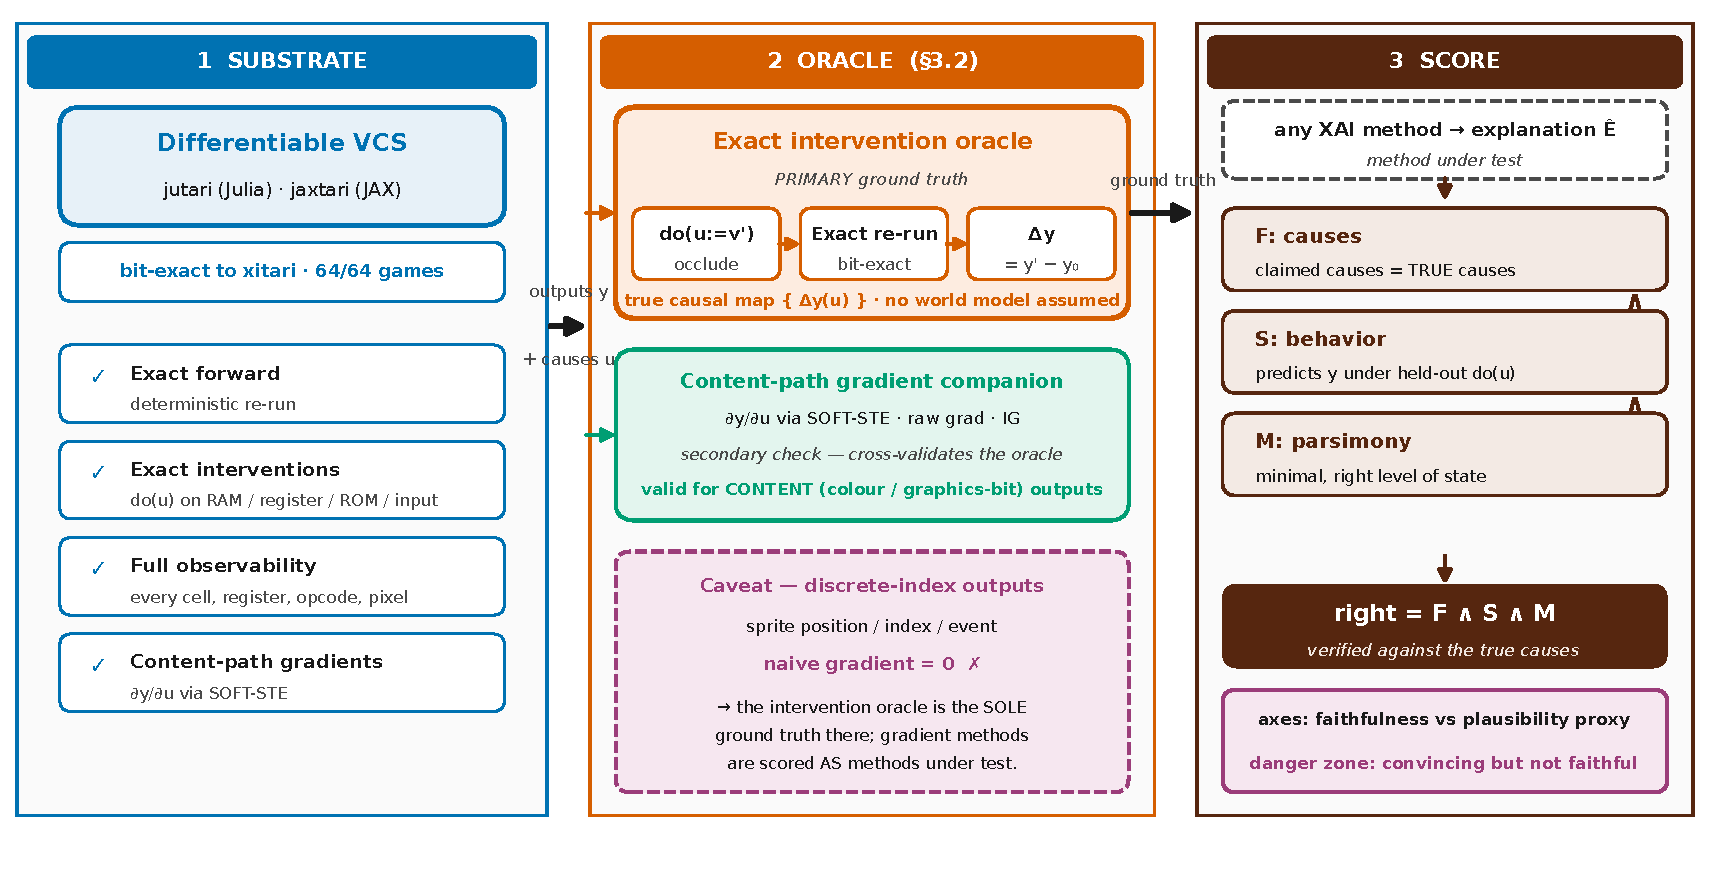
\includegraphics[width=\linewidth]{fig1_platform_oracle.pdf}
  \caption{\textbf{The measurement platform and its ground-truth oracle.} A
  differentiable, bit-exact port of the Atari VCS (left), realized as
  \texttt{jutari} (Julia) $\cdot$ \texttt{jaxtari} (JAX), gives four capabilities no neural
  network grants for free: exact forward, exact interventions $\mathrm{do}(u)$, full state
  observability, and content-path gradients. On it we build the oracle (centre): the primary
  intervention oracle of \Sectionname\ref{sec:oracle} (\Sectionname3.2), $\mathrm{do}(u{:=}v')\!\to\!\Delta y(u)$
  by bit-exact re-run, with a content-path gradient $\partial y/\partial u$ as a companion on
  the content path only. Any explanation $\hat{E}$ is scored by the correctness triad (right),
  $\text{right}=\mathrm{F}\wedge\mathrm{S}\wedge\mathrm{M}$, and reported on two axes,
  faithfulness against the oracle versus a plausibility proxy. Faithfulness aggregates
  correlation, sign and magnitude agreement, deletion/insertion area-under-curve, and
  precision at $k$ against the true causal top-$k$ (\Sectionname\ref{sec:triad}). A discrete index --- a
  sprite's position, set by strobe timing --- has a naive gradient that is zero under the hard
  forward map (Prop.~\ref{prop:zero}); for position, index, and event outputs the intervention
  oracle is the \emph{sole} ground truth and gradient methods are scored as methods under test.
  The schematic draws no experiment data. Data and oracle: see Supplement; oracle defined in
  \Sectionname\ref{sec:oracle} (\Sectionname3.2).}
  \label{fig:platform}
\end{figure}

\subsection{The differentiable, bit-exact VCS substrate}\label{sec:substrate}

The subject of this study is the Atari Video Computer System (VCS) itself, not a learned
agent. It is a complex real artifact never designed to be interpretable, yet whose every causal
dependency we can read off exactly. Paper~1 built it, a bit-exact, differentiable port of the
1977 VCS validated bit-for-bit against the \texttt{xitari} C++ reference on all 64 games of
the Paper-1 roster, in random-access memory and rendered screen, within the validated
conformance window~\cite{maier2025vcs,xitari}. Paper~1 is a technical companion that supplies
the mathematical proofs and experimental validation of the constructions we use here; no other
reference system like it exists anywhere, and no prior study has had the opportunity to
examine interpretability methods against this level of ground truth. We use the port in two
interchangeable, mutually cross-checked realizations, \texttt{jutari} (Julia) and
\texttt{jaxtari} (JAX/Python).

Paper~1 provides three execution modes. The \textbf{hard} mode is the bit-exact integer
machine, identical to the \texttt{xitari} C++ reference at every RAM byte and every screen
pixel. The \textbf{SOFT-STE} (straight-through estimator) mode keeps the forward pass
bit-identical to the hard mode at any finite temperature while routing a surrogate gradient
along the content path during the backward pass, a formulation whose forward equivalence
Paper~1 proves theoretically and validates experimentally across all 64 games. The
\textbf{soft} (fully relaxed) mode relaxes every discrete decision --- opcode dispatch via
a temperature-parameterised softmax, conditional branches via a sigmoid with steepness
$\alpha$, memory reads via a distance-weighted soft read --- into a fully differentiable
form. Paper~1 proves that the soft forward pass reproduces the hard machine bit-for-bit in
the limit $T \to 0^+$, $\alpha \to \infty$, and provides the temperature-limit error bound
$\|\Phi_{\mathrm{H}} - \Phi_{\mathrm{S}}\| \le (K-1)e^{-\Delta_{\min}/T} +
e^{-\alpha m_{\min}} + \rho e^{-1/T}$. At practical settings ($T \lesssim 0.14$, $\alpha
\gtrsim 6$), the soft mode remains forward-exact within machine precision for the validated
frame window; beyond those settings the forward pass diverges and the gradient quality
degrades.

The substrate grants four capabilities that no neural network offers for free. The first is
an exact forward map,
\begin{equation}
  y \;=\; \mathrm{VCS}\big(\mathrm{ROM},\, \mathrm{inputs}[0{:}t],\, s_0\big),
  \label{eq:vcs}
\end{equation}
that is, the output $y$ at step $t$, a pixel, a score, or a game event, is a deterministic
function of the cartridge bytes, the inputs up to $t$, and the initial state $s_0$, and
re-running reproduces $y$ to the bit. The second is exact interventions. We set any cause
$u$, a ROM byte, a RAM cell, a CPU/TIA/RIOT register, an opcode, or a joystick input, to any
value and re-run Eq.~\eqref{eq:vcs} deterministically. This realizes the causal operator
$\mathrm{do}(u)$ on a real machine rather than an assumed world model. The third is full
state observability, every bit of RAM and every register recorded along the trajectory, so
the ``activations'' we interpret are the program's own variables. The fourth is a gradient
$\partial y / \partial u$ that exists in all three modes. In SOFT-STE mode the gradient
routes through the content path via the straight-through estimator, while in soft mode the
gradient flows through every discrete decision, including the index boundary, at a cost of
numerical precision controlled by $T$ and $\alpha$. The inputs we
drive, the state we read and clamp, and the outputs we explain are the three faces a neural
interpretability study works with, so one substrate carries all three batteries.

We honor one boundary throughout. Paper-1 bit-exactness holds within a bounded frame window
on a fixed action stream, on the order of 30 frames of RAM and 60 frames of screen, and
every scored claim is taken inside that validated horizon. Long-horizon end-to-end gradients
are not needed for our single-step metrics, so we do not assume them.

\subsection{The ground-truth oracle}\label{sec:oracle}

The oracle is the heart of the method: for any output $y$ and any candidate cause $u$ it
returns the true effect of $u$ on $y$, against which every method is then scored. Its
primary construction is the exact intervention oracle: we intervene on $u$ by occlusion,
clamping, replacement, or resampling, re-run the machine deterministically, and record the
change in the output,
\begin{equation}
  \Delta y(u) \;=\; \mathrm{VCS}\big(\dots,\, \mathrm{do}(u{:=}v'),\, \dots\big) \;-\; y .
  \label{eq:doy}
\end{equation}
The true causal effect of a cause is thus the bit-exact difference its surgical edit makes
to the output, measured by actually running the altered machine, with no world model or
smoothness assumed. The collection $\{\Delta y(u)\}$ over all causes is the true causal map
of $y$, the reference for the faithfulness axis of every method.

The output $y$ comes in five regimes that fix what a method must predict and whether a
gradient is even meaningful. A \emph{content} output is a register, color, or graphics-bit
value that flows smoothly into the pixel, where the naive gradient is valid. A
\emph{position/index} output is a sprite, missile, or ball coordinate set by strobe timing,
where the naive gradient vanishes by Prop.~\ref{prop:zero} and only the bilinear-sampler
surrogate or the intervention oracle applies. An \emph{event} output is a discrete state
change, a collision latch or a life lost, also gradient-zero. A \emph{score} output is the
game's running counter, valid for the gradient only where it varies continuously. A
\emph{pixel} output is the rendered framebuffer value, content-valid where it tracks a smooth
cause and index-zero where it tracks a position. The Supplement lists, per game, which outputs
each method is scored on and the per-output gradient verdict.

The interventions that build the oracle are of distinct manifold kinds, and we state each
because the kind bounds what a score means. Occlusion and clamping are surgical but
\emph{off-manifold}: they can set a byte to a value the running program would never write.
Replacement from a donor trajectory is \emph{on-manifold}: the substituted value is one the
machine actually produced elsewhere. Resampling draws the cause from its own marginal over the
trajectory, and counterfactual edits are valid under the emulator by construction, since any
byte assignment yields a well-defined deterministic re-run. Off-manifold interventions are
acceptable for oracle scoring precisely because the oracle measures a \emph{causal} effect, not
a likelihood. The question is what the output would be if $u$ were $v'$. The bit-exact
machine answers it exactly for any $v'$, on- or off-manifold. Where a method's own claim is
about typical behavior rather than causal dependence we fall back to the on-manifold donor and
resampling variants and flag the choice in the Supplement.

The gradient $\partial y / \partial u$ through the differentiable substrate is a companion
construction. Its behaviour depends on the execution mode. In \textbf{SOFT-STE} mode, the
straight-through gradient routes to the content path only: register, colour, and graphics-bit
values that flow smoothly into the pixel agree with the intervention oracle, but a discrete
index --- a sprite's screen position set by the timing of a strobe write --- has a naive
gradient that vanishes under the hard forward map. In \textbf{soft} mode, the relaxation of
every discrete decision allows the gradient to flow through the index boundary as well, at a
cost controlled by the temperature $T$ and branch steepness $\alpha$. At the recommended
operating point ($T \approx 0.14$, $\alpha \gtrsim 6$), the soft gradient provides a
non-zero signal on position outputs while the forward pass remains bit-exact. As $T$ grows
or $\alpha$ shrinks, the forward pass diverges and the gradient becomes a looser surrogate.
We make the hard-map limit precise.

\begin{proposition}[Zero naive gradient for discrete-index outputs]\label{prop:zero}
Let an output $y$ depend on a cause $u$ only through a discrete index
$n(u)=\lfloor g(u)\rfloor\in\mathbb{Z}$, the integer count of colour clocks between a strobe
write and the position-counter reset that the VCS uses to place a sprite, missile, or ball,
with $g$ continuous, piecewise linear, and non-constant (strictly monotone on each linear
piece). Under the hard (bit-exact) forward map the rendered output is $y=h(n(u))$ for a fixed
render function $h$. Then $n(\cdot)$ is locally constant wherever $g(u)\notin\mathbb{Z}$, so
$\partial y/\partial u=0$ at every such point, and $y$ is discontinuous on the set
$\{u:g(u)\in\mathbb{Z}\}$, which is measure zero precisely because $g$ is strictly monotone on
each piece, and there the gradient is undefined. Hence the naive gradient is zero wherever the
derivative exists: an infinitesimal change in $u$ cannot move the sprite by a fractional
pixel. Any method that reduces to this naive gradient inherits the failure on position, index,
and event outputs.
\end{proposition}

The proposition states only the hard-map limit; it does not say that no useful gradient
exists. Paper~1~\cite{maier2025vcs} provides three constructions that escape it, each
corresponding to an execution mode. The \textbf{SOFT-STE} mode, through the straight-through
estimator, keeps the forward pass bit-exact at any finite temperature while routing a
non-zero gradient along the content path~\cite{bengio2013estimating,jang2017gumbel}; on
position outputs this gradient remains content-only and therefore zero. The \textbf{soft}
mode relaxes the discrete index boundary via a temperature-parameterised softmax, allowing
the gradient to flow through the index itself; the bilinear sampler is a special case of
this relaxation for spatial coordinates~\cite{jaderberg2015spatial}. The \textbf{bilinear
sampler} interpolates the index boundary to recover a usable position gradient without
relaxing the full machine~\cite{jaderberg2015spatial}. Paper~1 constructs and validates all
three, and proves the forward equivalence and temperature-limit bounds we assume.

Hence we have three companion gradient constructions, not one. The intervention oracle of
Eq.~\eqref{eq:doy} remains the primary ground truth across all modes. The SOFT-STE gradient
agrees with it on the content path but vanishes on position outputs; the soft gradient can
cover position outputs at the cost of temperature-dependent precision; and the bilinear
sampler provides a position gradient without relaxing the full machine. We score every
gradient-based method under all applicable modes and report the results separately. Where
the modes agree we report the common value; where they disagree the divergence itself is
informative about the method's reliance on gradient quality.

\subsection{Tiered ground truth and how we obtain it}\label{sec:tiers}

The ground truth comes in three tiers, and the tiering is not bookkeeping; it carries the
central argument of the paper. Tier~1 (T1) is the exact causal map of Eq.~\eqref{eq:doy},
derived internally from the substrate and available for all 64 games. Tier~2 (T2) is the
hardware roles and the read/write data-flow graph, also exact and internal across all 64
games. T1 and T2 are everything the machine \emph{is} and need no external label.

Tier~3 (T3) is different in kind, and that difference is the point. It attaches a
game-concept name to a cell or feature, ``the ball's $x$ position'' or ``the score,'' names
not computable from the substrate alone, because they are facts about what the program
\emph{means}, not what it \emph{does}. We import T3 from two public sources and make it
causal. AtariARI provides labels for 22 games, read from commented
disassemblies, with raw RAM coordinates not aligned to the rendered
position~\cite{anand2019unsupervised}; OCAtari covers more than 40 games and, in its RAM
mode, applies the render-time offsets that fix that misalignment~\cite{delfosse2023ocatari}.
We import both as candidates and verify each causally by setting the byte, re-rendering, and
confirming on the bit-exact framebuffer that the named object moves to the predicted place,
which upgrades a correlational label to a verified-causal one and auto-corrects the offsets;
further labels we discover by RAM-to-framebuffer correlation and intervention. The headline
core set is six games, Pong, Breakout, Space Invaders, Seaquest, Ms.\ Pac-Man, and Q*bert,
each carrying both sources, all in the Paper-1 bit-exact roster, together spanning
paddle-and-ball, shooter-with-shields, resource-meter, multi-agent-pursuit, and discrete-grid
logic. The remaining games form a breadth set scored on T1 and T2 only.

We are deliberate about what this buys us. All T3 labels are external and only verified,
never discovered from scratch, so a method that matches a supplied concept has aligned to a
given meaning, not recovered it. This is exactly why a probe can show that information is
\emph{present} without showing it is \emph{used}~\cite{hewitt2019designing}, and why our
intervention test, which asks whether the byte \emph{causes} the named object to move, is
strictly stronger than decoding it. Recovering the program's documentation and design from
the bare machine is a separate problem, the subject of the companion paper.

\subsection{The F\,$\wedge$\,S\,$\wedge$\,M correctness triad}\label{sec:triad}

A faithful attribution is not yet an understanding, and to make that a measurement we need an
operational criterion. We adopt one in the spirit of Marr's levels of
analysis~\cite{marr1982vision} and of Jonas and Kording's warning that finding structure is
not the same as explaining it~\cite{jonas2017could}: each axis is first a continuous score in
$[0,1]$, and the boolean ``right'' is a thresholded reading of those scores. We score an
explanation $\hat{E}$ of how an output $y$ arises by three numbers,
$\mathrm{F}_{\mathrm{score}}(\hat{E}),\,\mathrm{S}_{\mathrm{score}}(\hat{E}),\,
\mathrm{M}_{\mathrm{score}}(\hat{E})\in[0,1]$, and call it \emph{right} when all three clear
their thresholds,
\begin{equation}
  \mathrm{right}(\hat{E}) \;=\; \mathbf{1}\!\left[\,
  \mathrm{F}_{\mathrm{score}}\!\ge\!\tau_{\mathrm{F}} \,\wedge\,
  \mathrm{S}_{\mathrm{score}}\!\ge\!\tau_{\mathrm{S}} \,\wedge\,
  \mathrm{M}_{\mathrm{score}}\!\ge\!\tau_{\mathrm{M}}\,\right],
  \label{eq:triad}
\end{equation}
with $\tau_{\mathrm{F}}=\tau_{\mathrm{S}}=\tau_{\mathrm{M}}=0.5$ throughout. Results report the
continuous scores; the predicate is a derived summary, not the primary quantity. All three are
defined against the oracle, not against any method under test, which keeps the criterion
non-circular.

Faithfulness asks whether the claimed causes are the \emph{true} causes, scored against the
intervention oracle of Eq.~\eqref{eq:doy}. The per-record metric depends on the explanation's
output type, so $\mathrm{F}_{\mathrm{score}}$ is a single number assembled from three
type-matched primitives. The committed score is the bare effect-agreement primitive, not a
rescaled one: for a real-valued attribution map we report the Pearson (or Spearman, for ranked
outputs) correlation $\rho(\hat{E},\{\Delta y(u)\})$ between the attribution and the true causal
effects, scored \emph{raw}, so that a method whose attribution carries no causal signal lands at
$\rho=0$ rather than at the $0.5$ of an affine $\tfrac{1}{2}(1+\rho)$ remap. This is what makes
the position regime informative: under Prop.~\ref{prop:zero} the naive gradient is identically
zero there, its correlation with the oracle is $0$, and the reported faithfulness is therefore
$0.00$ and not a $0.5$ floor. The two committed estimators differ only in how the raw
correlation is summarized across the six core games. Phase~B reports the raw correlation
directly (e.g.\ occlusion at $\rho=0.482$), so a negative correlation is recorded as a negative
number; Phase~A's single-unit and tuning analyses, where per-game correlations can be negative,
report the per-game correlation clipped at $0$ and then averaged across games (e.g.\ the tuning
analysis A3, lowest in Phase~A at $0.116$, the clip-at-zero mean of six per-game correlations
that include negatives). For the same attribution map we also report, as quality measures,
deletion/insertion area-under-curve and precision at $k$ against the true causal top-$k$,
$\mathrm{P@}k=|\,\mathrm{top}_k(\hat{E})\cap\mathrm{top}_k(\{\Delta y(u)\})\,|/k$. For a
graph-valued explanation (Phase~A connectomics, Phase~C circuit discovery) we use the edge
$F_1$ against the true data-flow graph, the harmonic mean of precision and recall over recovered
edges, and for Phase~C patching and mediation the causal-effect-agreement correlation against
the true $\{\Delta y(u)\}$. The final $\mathrm{F}_{\mathrm{score}}$ is the per-record primary
metric averaged first within a game over its output records, then with equal weight across the
six core games, so no game-rich method dominates; confidence intervals are 95\% bootstrap over
games (\Sectionname\ref{sec:scoring}). The three Phases differ only in which primitive is primary: Phase~A
uses graph $F_1$ for the data-flow methods and the clip-at-zero mean correlation for the
single-unit and tuning analyses, Phase~B uses the raw effect-agreement correlation $\rho$ with
deletion/insertion AUC and $\mathrm{P@}k$ as the attribution map's quality measures, and Phase~C
uses the causal-effect-agreement correlation for patching and mediation and graph $F_1$ for
circuit discovery. The leaderboard score is therefore a single scalar per method, but it is
multi-metric in origin, and the per-method choice is recorded in the Supplement.

Sufficiency asks whether the explanation could regenerate the behavior under interventions it
has not seen. We treat $\mathrm{S}_{\mathrm{score}}$ as a held-out predictive estimator.
$\hat{E}$ is fit (or its causal sites read off) on a calibration set of interventions. It is
then asked to predict the true output $y'$ under a disjoint test set of held-out $\mathrm{do}(u)$
edits, with the prediction compared to the bit-exact re-run. The score is the fraction of
held-out interventions whose predicted $y'$ matches the true $y'$ within a fixed
output-type tolerance. The match is exact for discrete indices and events, and within a small
$\varepsilon$ band for continuous scores. Hence $\mathrm{S}_{\mathrm{score}}\in[0,1]$; a value
near zero means the explanation predicts no better than the unperturbed output. We deliberately
do not define it through interchange interventions or scrubbing. Those are themselves
mechanistic-interpretability methods under test in Phase~C, and using them would make the
criterion circular. Only Phase~B and Phase~C report $\mathrm{S}$. Its bootstrap intervals
follow \Sectionname\ref{sec:scoring}.

Minimality asks whether the explanation is parsimonious and lives at the algorithmic level of
the machine's own module decomposition. We define
$\mathrm{M}_{\mathrm{score}}=|U^\star|/|U_{\hat{E}}|\in(0,1]$, the ratio of the size of the
true minimal cause set $U^\star$, the smallest set of registers, RAM cells, opcodes, or
program variables whose intervention reproduces $y$, to the size $|U_{\hat{E}}|$ of the cause
set the explanation actually names. An explanation that names exactly the minimal set scores
$1$; one that records the whole machine state pays for every spurious cell. The target level
is the algorithmic unit, the register, RAM cell, opcode, module, or program variable, not the
pixel. This is why whole-state recording, which names all $128$ RAM cells where the true cause
set averages a handful, scores $\mathrm{M}_{\mathrm{score}}=0.07$ across the six core games:
its faithfulness is perfect because it withholds nothing, but it is maximally non-minimal.

Two reporting axes carry the headline comparison, faithfulness against the ground truth and a
plausibility proxy. The plausibility proxy is a documented, tradition-level value, not a
human-subjects measurement, and we report it as such. It is assigned per method tradition, not
per method instance, from the published evidence on how convincing each tradition's
explanations are taken to be, before any faithfulness score on our machine is computed, so the
proxy cannot be tuned to the result; the per-tradition assignment, its rubric, and its
sources are tabulated in the Supplement (Sec.~\ref{supp:plausibility}), where a sensitivity
analysis perturbs the proxy under additive, rank-preserving, rank-jittering, and
leave-one-tradition-out schemes and finds the faithfulness-versus-proxy rank correlation
stays negative throughout (from $-0.79$ to $-0.40$), so the headline contrast survives every
alternative proxy assignment we tried. Its job is to expose the danger zone of explanations with high
plausibility but low faithfulness, convincing yet wrong. Separating F, which the wiring
satisfies, from S and M, which the \emph{computation} must satisfy, is what lets us name,
later, the residual that faithfulness alone leaves behind.

\subsection{Methods under test, games, and aggregation}\label{sec:scoring}

We turn three traditions onto the machine and score each by the triad of
Eq.~\eqref{eq:triad}. The neuroscience battery (Phase~A) runs connectomics and data-flow
recovery, single-unit lesions, tuning curves, pairwise and global correlation structure,
pooled-activity spectra, Granger causality, dimensionality reduction, and whole-state
recording, scoring each against the known mechanism to quantify Kording's lesson at the
low-faithfulness baseline~\cite{jonas2017could}. The attribution and XAI
battery (Phase~B) runs gradient saliency and its variants, integrated gradients, occlusion,
perturbation masks, randomized masking, LIME, and Shapley-style
attribution~\cite{simonyan2014deep,sundararajan2017axiomatic,zeiler2014visualizing,fong2017interpretable,petsiuk2018rise,ribeiro2016why,lundberg2017unified};
Grad-CAM and its variants and attention
rollout~\cite{selvaraju2017gradcam,chattopadhyay2018gradcampp,abnar2020quantifying} require
neural layers or a learned policy and are recorded as not applicable. The
mechanistic-interpretability battery (Phase~C) runs activation patching and causal
mediation, interchange interventions and distributed alignment search, attribution and path
patching, automatic circuit discovery, sparse autoencoders, causal scrubbing, linear
probing with control tasks, and the logit and tuned
lens~\cite{vig2020investigating,meng2022locating,geiger2021causal,geiger2023finding,nanda2023attribution,wang2022interpretability,conmy2023towards,cunningham2023sparse,chan2022causal,alain2017understanding,hewitt2019designing,belrose2023eliciting}.

All faithfulness scoring runs on the six core games of Section~\ref{sec:tiers}, where the
oracle's re-runs are exact. Cell- and pixel-level scores, correlation, deletion and insertion
area-under-curve, and precision at $k$, are taken against T1 and need no T3. Only object- and
concept-level scores draw on the external T3 labels, and we flag every such score as
alignment-to-given, not discovery. We aggregate the committed per-game records into one row
per method on the shared faithfulness-versus-plausibility axes of the Results leaderboard.
The headline contrast is the position regime, where the naive gradient is zero under the hard
forward map by Prop.~\ref{prop:zero}.
There, causal and intervention methods average a faithfulness of $0.41$ against $0.07$ for
gradient and correlational methods, a gap of $0.34$. The per-method extreme places an
exact causal method, activation patching, at faithfulness $1.000$ and the field's default
saliency at $0.000$ on all six games. The popular method nonetheless carries the higher
plausibility proxy ($0.9$ versus $0.5$). Against these numbers the semantic gap is measured.

% =====================================================================
% BIBTEX-NEEDED: full entries for the keys cited above that are NOT yet
% in references.bib. The keys already present in references.bib that this
% section reuses are: xitari, jonas2017could, sundararajan2017axiomatic,
% selvaraju2017gradcam, chattopadhyay2018gradcampp, jaderberg2015spatial,
% jang2017gumbel, bengio2013estimating, delfosse2023ocatari.
% Please MERGE the following NEW entries (SM-only edit to references.bib):
% =====================================================================
%
% @article{maier2025vcs,
%   title   = {A bit-exact, differentiable port of the Atari 2600 Video Computer System},
%   author  = {Maier, Andreas and Bayer, Stefan and Krauss, Patrick},
%   journal = {(Paper 1; manuscript / preprint)},
%   year    = {2025},
%   note    = {jutari and jaxtari: 64/64 games bit-exact vs the xitari reference in RAM and screen}
% }
%
% @inproceedings{anand2019unsupervised,
%   title     = {Unsupervised State Representation Learning in Atari},
%   author    = {Anand, Ankesh and Racah, Evan and Ozair, Sherjil and Bengio, Yoshua and C{\^o}t{\'e}, Marc-Alexandre and Hjelm, R. Devon},
%   booktitle = {Advances in Neural Information Processing Systems (NeurIPS)},
%   year      = {2019}
% }
%
% @book{marr1982vision,
%   title     = {Vision: A Computational Investigation into the Human Representation and Processing of Visual Information},
%   author    = {Marr, David},
%   year      = {1982},
%   publisher = {W. H. Freeman and Company}
% }
%
% @inproceedings{simonyan2014deep,
%   title     = {Deep Inside Convolutional Networks: Visualising Image Classification Models and Saliency Maps},
%   author    = {Simonyan, Karen and Vedaldi, Andrea and Zisserman, Andrew},
%   booktitle = {International Conference on Learning Representations (ICLR) Workshop},
%   year      = {2014}
% }
%
% @inproceedings{zeiler2014visualizing,
%   title     = {Visualizing and Understanding Convolutional Networks},
%   author    = {Zeiler, Matthew D. and Fergus, Rob},
%   booktitle = {European Conference on Computer Vision (ECCV)},
%   year      = {2014},
%   pages     = {818--833}
% }
%
% @inproceedings{fong2017interpretable,
%   title     = {Interpretable Explanations of Black Boxes by Meaningful Perturbation},
%   author    = {Fong, Ruth C. and Vedaldi, Andrea},
%   booktitle = {IEEE International Conference on Computer Vision (ICCV)},
%   year      = {2017},
%   pages     = {3429--3437}
% }
%
% @inproceedings{petsiuk2018rise,
%   title     = {{RISE}: Randomized Input Sampling for Explanation of Black-box Models},
%   author    = {Petsiuk, Vitali and Das, Abir and Saenko, Kate},
%   booktitle = {British Machine Vision Conference (BMVC)},
%   year      = {2018}
% }
%
% @inproceedings{ribeiro2016why,
%   title     = {``Why Should I Trust You?'': Explaining the Predictions of Any Classifier},
%   author    = {Ribeiro, Marco Tulio and Singh, Sameer and Guestrin, Carlos},
%   booktitle = {Proceedings of the 22nd ACM SIGKDD International Conference on Knowledge Discovery and Data Mining},
%   year      = {2016},
%   pages     = {1135--1144}
% }
%
% @inproceedings{lundberg2017unified,
%   title     = {A Unified Approach to Interpreting Model Predictions},
%   author    = {Lundberg, Scott M. and Lee, Su-In},
%   booktitle = {Advances in Neural Information Processing Systems (NeurIPS)},
%   year      = {2017}
% }
%
% @inproceedings{abnar2020quantifying,
%   title     = {Quantifying Attention Flow in Transformers},
%   author    = {Abnar, Samira and Zuidema, Willem},
%   booktitle = {Proceedings of the 58th Annual Meeting of the Association for Computational Linguistics (ACL)},
%   year      = {2020},
%   pages     = {4190--4197}
% }
%
% @inproceedings{vig2020investigating,
%   title     = {Investigating Gender Bias in Language Models Using Causal Mediation Analysis},
%   author    = {Vig, Jesse and Gehrmann, Sebastian and Belinkov, Yonatan and Qian, Sharon and Nevo, Daniel and Singer, Yaron and Shieber, Stuart},
%   booktitle = {Advances in Neural Information Processing Systems (NeurIPS)},
%   year      = {2020}
% }
%
% @inproceedings{meng2022locating,
%   title     = {Locating and Editing Factual Associations in {GPT}},
%   author    = {Meng, Kevin and Bau, David and Andonian, Alex and Belinkov, Yonatan},
%   booktitle = {Advances in Neural Information Processing Systems (NeurIPS)},
%   year      = {2022}
% }
%
% @inproceedings{geiger2021causal,
%   title     = {Causal Abstractions of Neural Networks},
%   author    = {Geiger, Atticus and Lu, Hanson and Icard, Thomas and Potts, Christopher},
%   booktitle = {Advances in Neural Information Processing Systems (NeurIPS)},
%   year      = {2021}
% }
%
% @inproceedings{geiger2023finding,
%   title     = {Finding Alignments Between Interpretable Causal Variables and Distributed Neural Representations},
%   author    = {Geiger, Atticus and Wu, Zhengxuan and Potts, Christopher and Icard, Thomas and Goodman, Noah D.},
%   booktitle = {Proceedings of the Third Conference on Causal Learning and Reasoning (CLeaR)},
%   year      = {2024}
% }
%
% @misc{nanda2023attribution,
%   title        = {Attribution Patching: Activation Patching at Industrial Scale},
%   author       = {Nanda, Neel},
%   year         = {2023},
%   howpublished = {\url{https://www.neelnanda.io/mechanistic-interpretability/attribution-patching}}
% }
%
% @inproceedings{wang2022interpretability,
%   title     = {Interpretability in the Wild: A Circuit for Indirect Object Identification in {GPT-2} Small},
%   author    = {Wang, Kevin and Variengien, Alexandre and Conmy, Arthur and Shlegeris, Buck and Steinhardt, Jacob},
%   booktitle = {International Conference on Learning Representations (ICLR)},
%   year      = {2023}
% }
%
% @inproceedings{conmy2023towards,
%   title     = {Towards Automated Circuit Discovery for Mechanistic Interpretability},
%   author    = {Conmy, Arthur and Mavor-Parker, Augustine N. and Lynch, Aengus and Heimersheim, Stefan and Garriga-Alonso, Adri{\`a}},
%   booktitle = {Advances in Neural Information Processing Systems (NeurIPS)},
%   year      = {2023}
% }
%
% @misc{cunningham2023sparse,
%   title         = {Sparse Autoencoders Find Highly Interpretable Features in Language Models},
%   author        = {Cunningham, Hoagy and Ewart, Aidan and Riggs, Logan and Huben, Robert and Sharkey, Lee},
%   year          = {2023},
%   eprint        = {2309.08600},
%   archivePrefix = {arXiv},
%   primaryClass  = {cs.LG}
% }
%
% @misc{chan2022causal,
%   title        = {Causal Scrubbing: A Method for Rigorously Testing Interpretability Hypotheses},
%   author       = {Chan, Lawrence and Garriga-Alonso, Adri{\`a} and Goldowsky-Dill, Nicholas and Greenblatt, Ryan and Nitishinskaya, Jenny and Radhakrishnan, Ansh and Shlegeris, Buck and Thomas, Nate},
%   year         = {2022},
%   howpublished = {AI Alignment Forum}
% }
%
% @inproceedings{alain2017understanding,
%   title     = {Understanding Intermediate Layers Using Linear Classifier Probes},
%   author    = {Alain, Guillaume and Bengio, Yoshua},
%   booktitle = {International Conference on Learning Representations (ICLR) Workshop},
%   year      = {2017}
% }
%
% @inproceedings{hewitt2019designing,
%   title     = {Designing and Interpreting Probes with Control Tasks},
%   author    = {Hewitt, John and Liang, Percy},
%   booktitle = {Proceedings of the 2019 Conference on Empirical Methods in Natural Language Processing (EMNLP)},
%   year      = {2019},
%   pages     = {2733--2743}
% }
%
% @misc{belrose2023eliciting,
%   title         = {Eliciting Latent Predictions from Transformers with the Tuned Lens},
%   author        = {Belrose, Nora and Furman, Zach and Smith, Logan and Halawi, Danny and Ostrovsky, Igor and McKinney, Lev and Biderman, Stella and Steinhardt, Jacob},
%   year          = {2023},
%   eprint        = {2303.08112},
%   archivePrefix = {arXiv},
%   primaryClass  = {cs.LG}
% }

% 09_endmatter.tex — End matter (data/code availability, author contributions,
% competing interests, acknowledgements). Drafted by item P2-E8-9 (P2 Sprint 7).
% Voice: ../STYLE.md (Andreas Maier). Requirements: document_check.md §D.
% Availability statements kept consistent with the repro bundle (E9). The MIT-on-
% acceptance line is the project's release policy. Author contributions are a
% CRediT-style placeholder pending final author list (provisional in main.tex).
% Honour the honesty contract: the benchmark releases the scoring suite, oracle, and
% metrics; no semantic-recovery claim is made here (that is Paper 4).

\backmatter

\bmhead{Data availability}
The interpretability scores reported here are derived from the committed analysis
records under \texttt{tools/xai\_study/} (the per-method, per-game §R records and the
aggregated cross-tradition leaderboard~\cite{leaderboardP2,faithfuldemoP2}); every
quantitative claim in the Article reads from one of these committed artifacts, and no
number is re-run or estimated. The game cartridges used as the subject are
third-party Atari~2600 ROMs that we do \emph{not} redistribute; following the
practice of the underlying emulator port~\cite{maier2025vcs}, we provide the SHA-256
hashes of each ROM and the \texttt{AutoROM} retrieval procedure so that the exact
binaries can be reproduced independently. The recorded state trajectories used to
train the sparse autoencoders and to run the patching and probing experiments are
regenerated deterministically from those ROMs and the published action streams.

\bmhead{Code availability}
The differentiable, bit-exact emulator in its two interchangeable realizations
(\texttt{jutari}, Julia; \texttt{jaxtari}, JAX/Python) and the ground-truth
intervention oracle are described in the companion port paper~\cite{maier2025vcs}.
The interpretability benchmark introduced here---the scoring suite, the F\,$\wedge$\,
S\,$\wedge$\,M triad metrics, and the per-phase method implementations
(\texttt{tools/xai\_study/})---will be released as a reusable open-source artifact.
The full source for the emulator, the oracle, and the benchmark will be made
available under the MIT license upon acceptance.

\bmhead{Author contributions}
\emph{[CRediT placeholder, to be finalised with the author list.]} A.M. conceived the
study, designed the ground-truth audit and the F\,$\wedge$\,S\,$\wedge$\,M triad, and
wrote the manuscript. S.B. and P.K. contributed to the method design, the
substrate and oracle, and the analysis. All authors discussed the results,
interpreted the semantic-gap finding, and revised the manuscript. The
differentiability framing and the gradient-faithfulness analysis were developed
jointly with P.K.

\bmhead{Competing interests}
The authors declare no competing interests.

\bmhead{Ethics and broader impact}
This study uses no human-subjects data; the human-plausibility axis is a documented
method-tradition proxy rather than a measurement, and we report it as such. The
subject is a fully deterministic, hand-coded program with no learned policy, so no
agent is trained. Interpretability methods are dual-use, in that a tool that audits a
system can also be used to probe it; our contribution is a calibration that makes
explanation claims more, not less, trustworthy, and we release it openly to that end.
The game cartridges are not redistributed.

\bmhead{Acknowledgements}
\emph{[To be completed: funding sources and compute allocations.]} The authors thank
the maintainers of the AtariARI~\cite{anand2019unsupervised} and
OCAtari~\cite{delfosse2023ocatari} projects, whose game-concept labels we imported as
external candidates and only causally verified, and the maintainers of the
\texttt{xitari} reference emulator~\cite{xitari} against which the substrate is
validated bit-for-bit. The pilots were run locally; the full sweeps used the
institutional compute cluster.

% =====================================================================
% BIBTEX-NEEDED: this section introduces NO new keys. Every key cited above is
% already declared in a sibling section's BIBTEX-NEEDED block (SM to merge):
%   leaderboardP2          -> 04_results_A.tex
%   faithfuldemoP2         -> 07_results_compare.tex
%   maier2025vcs, xitari   -> 03_methods.tex
%   anand2019unsupervised  -> 03_methods.tex
%   delfosse2023ocatari    -> 03_methods.tex
% =====================================================================


%%=============================================================%%
%% Bibliography — existing references.bib, sn-nature style.
%%=============================================================%%
\bibliography{references}

%%=============================================================%%
%% Supplementary Information (S1–S6 + full SI figures).
%%=============================================================%%
%% supplement.tex — Supplementary Information for Paper 2 (xai_2_interpretability).
%%
%% SCRUM note (P2-R-SUPP): this fragment is \input{} into the main paper by the SM
%% integration write (R6 wires %% supplement.tex — Supplementary Information for Paper 2 (xai_2_interpretability).
%%
%% SCRUM note (P2-R-SUPP): this fragment is \input{} into the main paper by the SM
%% integration write (R6 wires %% supplement.tex — Supplementary Information for Paper 2 (xai_2_interpretability).
%%
%% SCRUM note (P2-R-SUPP): this fragment is \input{} into the main paper by the SM
%% integration write (R6 wires \input{supplement/supplement} into main.tex). It is also
%% a self-contained \input target: the six S-files below carry all SI content the main
%% paper promises (improvement_instructions P0#2, P0#4; P1#13, P1#14, P1#21; P3#35, P3#36).
%%
%% It re-uses, but does not re-derive, the §3 F/S/M definitions (S03 is authoritative)
%% and the canonical method count "30 interpretability methods + the oracle positive
%% control = 31 rows" (S07 is authoritative). Every reported number traces to a committed
%% record under tools/xai_study/compare/out/ (verifiable via the §6.5 traceability table
%% of REPRODUCIBILITY.md and re-derived by S5 below).
%%
%% Standalone compile (for review, before R6 wires it into main): wrap this file in the
%% sn-jnl preamble of a scratch driver (\documentclass[sn-nature,pdflatex]{sn-jnl} +
%% graphicx, booktabs, multirow, amsmath, longtable) and \input{supplement}; the tables
%% render without overfull boxes and the two SI figures resolve from ../figures/.

\clearpage
\appendix

%% Breakable monospaced JSON key: lets long under_scored keys wrap inside narrow table
%% columns. Used by S5 (number provenance). Defined here so the S-files stay self-contained.
\providecommand{\jkey}[1]{\texttt{\expandafter\jkeyaux#1\relax}}
\makeatletter
\def\jkeyaux#1{\ifx\relax#1\else
  \ifx_#1\discretionary{}{}{}\char`\_\else
    \ifx.#1\discretionary{}{}{}.\else#1\fi\fi
  \expandafter\jkeyaux\fi}
\makeatother

\section*{Supplementary Information}
\setcounter{table}{0}
\setcounter{figure}{0}
\renewcommand{\thetable}{S\arabic{table}}
\renewcommand{\thefigure}{S\arabic{figure}}
\renewcommand{\thesection}{S\arabic{section}}
\setcounter{section}{0}

This Supplementary Information records what the main paper summarizes. We give the
per-method protocols (\Sectionname\ref{supp:protocols}) and the leaderboard schema with its glossary
(\Sectionname\ref{supp:schema}). We give the coverage and applicability of every method across games
and output regimes (\Sectionname\ref{supp:coverage}). We map each headline claim to its evidence
(\Sectionname\ref{supp:claims}). We trace the provenance of every headline number down to the record
file and command that produced it (\Sectionname\ref{supp:provenance}). We state plainly what the
paper does not claim (\Sectionname\ref{supp:notclaimed}). We give the plausibility-proxy rubric and
its sensitivity analysis (\Sectionname\ref{supp:plausibility}). The main text shows simplified forms
of two diagnostic figures; we reproduce both here at full resolution
(Figs.~\ref{supp:fig:repmap} and~\ref{supp:fig:taxonomy}).
The correctness triad $\mathrm{F}\wedge\mathrm{S}\wedge\mathrm{M}$ used throughout is the
one defined in the main Methods (\Sectionname\ref{sec:triad}); we reference it here rather than restating it. The
benchmark scores 30 interpretability methods together with the intervention oracle (\Sectionname\ref{sec:oracle})
as a positive control, for 31 leaderboard rows in total.

\input{supplement/S1_per_method_protocols}
\input{supplement/S2_benchmark_schema}
\input{supplement/S3_coverage_applicability}
\input{supplement/S4_claims_evidence}
\input{supplement/S5_number_provenance}
\input{supplement/S6_not_claimed}
\input{supplement/S7_plausibility}
 into main.tex). It is also
%% a self-contained \input target: the six S-files below carry all SI content the main
%% paper promises (improvement_instructions P0#2, P0#4; P1#13, P1#14, P1#21; P3#35, P3#36).
%%
%% It re-uses, but does not re-derive, the §3 F/S/M definitions (S03 is authoritative)
%% and the canonical method count "30 interpretability methods + the oracle positive
%% control = 31 rows" (S07 is authoritative). Every reported number traces to a committed
%% record under tools/xai_study/compare/out/ (verifiable via the §6.5 traceability table
%% of REPRODUCIBILITY.md and re-derived by S5 below).
%%
%% Standalone compile (for review, before R6 wires it into main): wrap this file in the
%% sn-jnl preamble of a scratch driver (\documentclass[sn-nature,pdflatex]{sn-jnl} +
%% graphicx, booktabs, multirow, amsmath, longtable) and %% supplement.tex — Supplementary Information for Paper 2 (xai_2_interpretability).
%%
%% SCRUM note (P2-R-SUPP): this fragment is \input{} into the main paper by the SM
%% integration write (R6 wires \input{supplement/supplement} into main.tex). It is also
%% a self-contained \input target: the six S-files below carry all SI content the main
%% paper promises (improvement_instructions P0#2, P0#4; P1#13, P1#14, P1#21; P3#35, P3#36).
%%
%% It re-uses, but does not re-derive, the §3 F/S/M definitions (S03 is authoritative)
%% and the canonical method count "30 interpretability methods + the oracle positive
%% control = 31 rows" (S07 is authoritative). Every reported number traces to a committed
%% record under tools/xai_study/compare/out/ (verifiable via the §6.5 traceability table
%% of REPRODUCIBILITY.md and re-derived by S5 below).
%%
%% Standalone compile (for review, before R6 wires it into main): wrap this file in the
%% sn-jnl preamble of a scratch driver (\documentclass[sn-nature,pdflatex]{sn-jnl} +
%% graphicx, booktabs, multirow, amsmath, longtable) and \input{supplement}; the tables
%% render without overfull boxes and the two SI figures resolve from ../figures/.

\clearpage
\appendix

%% Breakable monospaced JSON key: lets long under_scored keys wrap inside narrow table
%% columns. Used by S5 (number provenance). Defined here so the S-files stay self-contained.
\providecommand{\jkey}[1]{\texttt{\expandafter\jkeyaux#1\relax}}
\makeatletter
\def\jkeyaux#1{\ifx\relax#1\else
  \ifx_#1\discretionary{}{}{}\char`\_\else
    \ifx.#1\discretionary{}{}{}.\else#1\fi\fi
  \expandafter\jkeyaux\fi}
\makeatother

\section*{Supplementary Information}
\setcounter{table}{0}
\setcounter{figure}{0}
\renewcommand{\thetable}{S\arabic{table}}
\renewcommand{\thefigure}{S\arabic{figure}}
\renewcommand{\thesection}{S\arabic{section}}
\setcounter{section}{0}

This Supplementary Information records what the main paper summarizes. We give the
per-method protocols (\Sectionname\ref{supp:protocols}) and the leaderboard schema with its glossary
(\Sectionname\ref{supp:schema}). We give the coverage and applicability of every method across games
and output regimes (\Sectionname\ref{supp:coverage}). We map each headline claim to its evidence
(\Sectionname\ref{supp:claims}). We trace the provenance of every headline number down to the record
file and command that produced it (\Sectionname\ref{supp:provenance}). We state plainly what the
paper does not claim (\Sectionname\ref{supp:notclaimed}). We give the plausibility-proxy rubric and
its sensitivity analysis (\Sectionname\ref{supp:plausibility}). The main text shows simplified forms
of two diagnostic figures; we reproduce both here at full resolution
(Figs.~\ref{supp:fig:repmap} and~\ref{supp:fig:taxonomy}).
The correctness triad $\mathrm{F}\wedge\mathrm{S}\wedge\mathrm{M}$ used throughout is the
one defined in the main Methods (\Sectionname\ref{sec:triad}); we reference it here rather than restating it. The
benchmark scores 30 interpretability methods together with the intervention oracle (\Sectionname\ref{sec:oracle})
as a positive control, for 31 leaderboard rows in total.

\input{supplement/S1_per_method_protocols}
\input{supplement/S2_benchmark_schema}
\input{supplement/S3_coverage_applicability}
\input{supplement/S4_claims_evidence}
\input{supplement/S5_number_provenance}
\input{supplement/S6_not_claimed}
\input{supplement/S7_plausibility}
; the tables
%% render without overfull boxes and the two SI figures resolve from ../figures/.

\clearpage
\appendix

%% Breakable monospaced JSON key: lets long under_scored keys wrap inside narrow table
%% columns. Used by S5 (number provenance). Defined here so the S-files stay self-contained.
\providecommand{\jkey}[1]{\texttt{\expandafter\jkeyaux#1\relax}}
\makeatletter
\def\jkeyaux#1{\ifx\relax#1\else
  \ifx_#1\discretionary{}{}{}\char`\_\else
    \ifx.#1\discretionary{}{}{}.\else#1\fi\fi
  \expandafter\jkeyaux\fi}
\makeatother

\section*{Supplementary Information}
\setcounter{table}{0}
\setcounter{figure}{0}
\renewcommand{\thetable}{S\arabic{table}}
\renewcommand{\thefigure}{S\arabic{figure}}
\renewcommand{\thesection}{S\arabic{section}}
\setcounter{section}{0}

This Supplementary Information records what the main paper summarizes. We give the
per-method protocols (\Sectionname\ref{supp:protocols}) and the leaderboard schema with its glossary
(\Sectionname\ref{supp:schema}). We give the coverage and applicability of every method across games
and output regimes (\Sectionname\ref{supp:coverage}). We map each headline claim to its evidence
(\Sectionname\ref{supp:claims}). We trace the provenance of every headline number down to the record
file and command that produced it (\Sectionname\ref{supp:provenance}). We state plainly what the
paper does not claim (\Sectionname\ref{supp:notclaimed}). We give the plausibility-proxy rubric and
its sensitivity analysis (\Sectionname\ref{supp:plausibility}). The main text shows simplified forms
of two diagnostic figures; we reproduce both here at full resolution
(Figs.~\ref{supp:fig:repmap} and~\ref{supp:fig:taxonomy}).
The correctness triad $\mathrm{F}\wedge\mathrm{S}\wedge\mathrm{M}$ used throughout is the
one defined in the main Methods (\Sectionname\ref{sec:triad}); we reference it here rather than restating it. The
benchmark scores 30 interpretability methods together with the intervention oracle (\Sectionname\ref{sec:oracle})
as a positive control, for 31 leaderboard rows in total.

\section{Per-method protocols}\label{supp:protocols}

This section records five things for each method under test. It records the exact objects the
method consumes and produces, the reference it is scored against, its sampling or optimization
budget, the metric that turns its output into a faithfulness score, and the committed record
file (version-controlled, in the released repository) that holds the per-game results. All methods share one evaluation contract. We state that
contract once and then specialize it per method. Every method receives the same bit-exact VCS
state on each game of the scored set. We state the contract on the six core games
(\texttt{breakout}, \texttt{ms\_pacman}, \texttt{pong}, \texttt{qbert}, \texttt{seaquest},
\texttt{space\_invaders}), which carry the full tiered ground truth and the exact oracle and
serve as the running example; the aggregate leaderboard scores extend the identical protocol
to the 42-game scored set of \Sectionname\ref{supp:scoredset}. That state is not the boot screen.
It is a shared gameplay state, produced by a single seeded random-action stream (seed~$0$) run
for a $90$-frame prefix and then rolled forward for a $15$-frame analysis horizon. The stream is
deterministic, so every method sees the identical state on each game, and the run is asserted
bit-exact per game. An oracle cause-density gate screens the state before any method runs. The
gate counts how many candidate causes move the output above a floor and rejects states with too
few, so a near-flat oracle column cannot pass. This gate is what turns a degenerate frame into a
usable one; on \texttt{seaquest} it raises the count of live candidate causes from $2$ to $19$.
The candidate-cause set is the machine's own state. This set is the RAM bytes together with the
CPU registers and the TIA and RIOT registers exposed by the substrate. The output every method
attributes over is a shared screen-buffer region read at the end of the analysis horizon, not a
single hand-picked pixel. The reference is the intervention oracle of \Sectionname\ref{sec:oracle},
evaluated by exact re-runs of the emulator under $\mathrm{do}(u)$. A method that
cannot be applied to a given output regime is recorded as not-applicable rather than scored
as zero. An empty result is therefore never read as a wrong one. Faithfulness is the F
axis of the main-text triad (\Sectionname\ref{sec:triad}); we reference that definition and do not restate it.
Records live under \texttt{tools/xai\_study/<phase>/out/}; the aggregate they feed is
\texttt{tools/xai\_study/compare/out/leaderboard.json}.
Table~\ref{supp:leaderboard} consolidates the triad scores for all thirty methods and the
oracle positive control in one place; the per-method protocols follow.

\begin{table*}[t]
\centering
\caption{\textbf{Consolidated leaderboard: all methods, all triad axes.} One row per method
across the three phases, plus the intervention oracle as a positive control. $F$ is
faithfulness (Pearson correlation against the oracle, with the bootstrap-over-games 95\% CI in
brackets), $S$ is sufficiency, $M$ is minimality, all as defined in \Sectionname\ref{sec:triad};
Plaus is the elicited plausibility prior and $n$ is the number of scored games. Attribution
methods that emit only a saliency have no defined $S$ or $M$ and are marked ``---''; A5
(field potentials) and A7 (dimensionality reduction) likewise lack the $S$/$M$ decomposition.
Values are transcribed from \texttt{tools/xai\_study/compare/out/leaderboard.json} (the
committed numbers of record).}
\label{supp:leaderboard}
\footnotesize
\setlength{\tabcolsep}{4pt}
\begin{tabularx}{\textwidth}{@{}Xccccccc@{}}
\toprule
Method & Phase & Tradition & $F$ (95\% CI) & $S$ & $M$ & Plaus & $n$ \\
\midrule
A1 connectomics & A & intervention & 0.207 [0.130, 0.293] & 0.971 & 0.967 & 0.55 & 35 \\
A2 lesions & A & intervention & 0.965 [0.942, 0.983] & 0.591 & 1.000 & 0.55 & 42 \\
A3 tuning curves & A & correlational & 0.213 [0.136, 0.295] & 0.200 & 0.928 & 0.80 & 42 \\
A4 spike-word / pairwise & A & correlational & 0.225 [0.166, 0.283] & 0.133 & 0.363 & 0.80 & 34 \\
A5 field potentials & A & correlational & 0.376 [0.323, 0.428] & --- & --- & 0.80 & 40 \\
A6 Granger & A & correlational & 0.136 [0.091, 0.184] & 0.884 & 0.647 & 0.80 & 35 \\
A7 dim.\ reduction & A & dim.\ red. & 0.519 [0.457, 0.581] & --- & --- & 0.75 & 42 \\
A8 whole-state & A & descriptive & 1.000 [1.000, 1.000] & 1.000 & 0.075 & 0.30 & 42 \\
\midrule
Vanilla saliency & B & gradient & 0.380 [0.316, 0.445] & --- & --- & 0.90 & 42 \\
smoothgrad & B & gradient & 0.380 [0.317, 0.445] & --- & --- & 0.90 & 42 \\
Guided backprop & B & gradient & 0.322 [0.267, 0.375] & --- & --- & 0.90 & 42 \\
Grad$\times$Input / DeepLIFT & B & gradient & 0.486 [0.448, 0.526] & --- & --- & 0.90 & 42 \\
Integrated Gradients & B & gradient & 0.379 [0.314, 0.444] & --- & --- & 0.90 & 42 \\
Expected Gradients & B & gradient & 0.175 [0.110, 0.240] & --- & --- & 0.90 & 42 \\
kernelshap & B & gradient & 0.652 [0.596, 0.709] & --- & --- & 0.90 & 42 \\
lime & B & gradient & 0.644 [0.582, 0.705] & --- & --- & 0.90 & 42 \\
rise & B & gradient & 0.552 [0.500, 0.600] & --- & --- & 0.90 & 42 \\
occlusion & B & intervention & 0.687 [0.624, 0.746] & --- & --- & 0.55 & 42 \\
Extremal perturbation & B & intervention & 0.461 [0.410, 0.513] & --- & --- & 0.55 & 42 \\
On-distribution counterfactual & B & intervention & 0.433 [0.343, 0.522] & --- & --- & 0.55 & 42 \\
\midrule
Activation patching & C & causal & 1.000 [1.000, 1.000] & --- & --- & 0.50 & 42 \\
Causal scrubbing & C & causal & 0.979 [0.940, 1.000] & 0.979 & 0.814 & 0.50 & 42 \\
Interchange interventions (DAS) & C & causal & 1.000 [1.000, 1.000] & --- & --- & 0.50 & 42 \\
Logit / tuned lens & C & causal & 0.820 [0.768, 0.871] & --- & 0.224 & 0.50 & 42 \\
Path patching & C & causal & 0.580 [0.452, 0.710] & --- & --- & 0.50 & 42 \\
ACDC & C & causal & 0.625 [0.514, 0.730] & 0.299 & 1.000 & 0.50 & 35 \\
Attribution patching & C & gradient & 0.456 [0.345, 0.573] & --- & --- & 0.90 & 42 \\
Linear probing (+ control) & C & probing & 0.240 [0.153, 0.346] & --- & 0.932 & 0.85 & 42 \\
NMF / PCA dictionaries & C & dim.\ red. & 0.102 [0.049, 0.160] & 0.751 & 0.966 & 0.75 & 42 \\
Sparse autoencoder & C & dim.\ red. & 0.153 [0.096, 0.218] & 0.183 & 0.934 & 0.75 & 40 \\
\midrule
Intervention oracle & --- & oracle & 1.000 [1.000, 1.000] & 1.000 & 1.000 & 1.00 & 1 \\
\bottomrule
\end{tabularx}
\end{table*}

The neuroscience analyses (Phase~A) treat the running machine as a brain. It asks how far
each classical analysis recovers the known mechanism on the shared gameplay state. Each
method's baseline is the exact data-flow graph or causal role that the substrate makes
available. Its budget is the scored set (\Sectionname\ref{supp:scoredset}) unless noted,
with the six-game core as the running example, and its scoring metric is named in
Table~\ref{supp:tab:phaseA}. One core cell is honestly degenerate. On \texttt{ms\_pacman} the
pairwise analysis (A4) finds no coupled candidate pair to score at that frame, so its
\texttt{ms\_pacman} value is uninformative rather than a failure; the other five games carry
it.

\begin{table}[t]
\centering
\caption{\textbf{Phase~A protocols (neuroscience analyses).} One row per method. The columns
give the input it reads, the reference it is scored against, the sampling or intervention
budget, the scoring metric, and the committed record. All eight run on the scored set
(\Sectionname\ref{supp:scoredset}), with the six core games as the running example;
faithfulness is the F axis of \Sectionname\ref{sec:triad}. The whole-state recording (A8) is included as a
descriptive upper bound on coverage. Its faithfulness $F$ is trivial, so we read it for its
minimality $M$.}
\label{supp:tab:phaseA}
\scriptsize
\setlength{\tabcolsep}{4pt}
\begin{tabular}{@{}p{1.7cm}p{2.6cm}p{1.9cm}p{2.6cm}p{1.0cm}@{}}
\toprule
Method & Input / candidate causes & Reference & Scoring metric & Record \\
\midrule
A1 connectomics & RAM/register activity over trajectory & data-flow graph & data-flow graph $F_1$ vs.\ oracle & A1 \\
A2 lesions & single-cell knockouts via $\mathrm{do}(u)$ & true causal role & lesion-importance $\rho$ vs.\ role & A2 \\
A3 tuning curves & per-cell response vs.\ variable & variable coupling & $1-$ spurious-tuning rate & A3 \\
A4 spike-word / pairwise & pairwise cell correlations & true coupling & corr.\ $\rho$ vs.\ coupling & A4 \\
A5 field potentials & pooled-activity spectra & true causal share & $1-$ clock-explained var. & A5 \\
A6 Granger & directed lag structure & true data-flow & $1-$ false-edge rate & A6 \\
A7 dim.\ reduction & NMF/PCA over activity & known variables & NMF matched-component frac. & A7 \\
A8 whole-state & full state record & oracle decomp. & minimality $M$ vs.\ oracle & A8 \\
\bottomrule
\end{tabular}

\smallskip
\noindent\scriptsize Records: \texttt{tools/xai\_study/phaseA\_kording/out/A\{1..8\}\_*}; all
eight run on the 42-game scored set (\Sectionname\ref{supp:scoredset}), with the six core
games as the running example (\jkey{n_games} per method in \jkey{leaderboard.json}).
\end{table}

The attribution methods (Phase~B) run the everyday XAI toolbox over the same gameplay state.
These methods produce a real-valued saliency or attribution over the candidate-cause set.
We score that output by Pearson correlation against the oracle attribution. The gradient family
runs with the bilinear sub-pixel sampler turned on, so it is scored on a real position gradient
and not on the naive one. The naive gradient of the discrete position output is provably zero
(Prop.~\ref{prop:zero}); the sampler restores a finite gradient, but the restored gradient is
low and mixed in faithfulness rather than a fix. Expected Gradients draws its reference pool
from the states of the same seeded gameplay trajectory, not from a synthetic baseline. Two cells
are honestly degenerate and recorded as such. The on-distribution counterfactual returns a zero
delta on \texttt{space\_invaders}, \texttt{ms\_pacman}, and \texttt{qbert}, where its perturbation
does not move the shared output at that frame; those cells are marked not-valid rather than
scored. Expected Gradients scores low on the content regime of every game except \texttt{pong},
because the causal byte it should land on is static there. The budgets that matter are the
Monte-Carlo or perturbation counts of the sampling estimators, recorded per method in
Table~\ref{supp:tab:phaseB}. The seed-dispersion of the stochastic members is carried in
\texttt{leaderboard\_ci.csv} (\texttt{seed\_sd}, \texttt{seed\_sd\_source}) and reproduced
in \Sectionname\ref{supp:provenance}.

\begin{table}[t]
\centering
\caption{\textbf{Phase~B protocols (attribution methods).} Each method emits a saliency over
the candidate-cause set. We score it by Pearson correlation against the oracle attribution
(\Sectionname\ref{sec:oracle}). The reference is shared and the budget is the scored set of
\Sectionname\ref{supp:scoredset} (six core games as the running example). The budget column records the
sampling or perturbation count that drives each estimator. The seed column flags which
methods carry an independent-seed dispersion in \texttt{leaderboard\_ci.csv}.}
\label{supp:tab:phaseB}
\scriptsize
\setlength{\tabcolsep}{4pt}
\begin{tabular}{@{}p{2.9cm}p{1.75cm}p{4.3cm}p{1.15cm}@{}}
\toprule
Method & Tradition & Budget / hyperparameters & Seed sd \\
\midrule
Vanilla saliency & gradient & single backward pass & --- \\
smoothgrad & gradient & noise-averaged gradient; $\sigma$-robustness committed & 0.0 \\
Guided backprop & gradient & single guided pass & --- \\
Grad$\times$Input / DeepLIFT & gradient & DeepLIFT reference-difference & --- \\
Integrated Gradients & gradient & path integral, baseline = zero state & --- \\
Expected Gradients & gradient & expectation over baselines (refits) & yes \\
kernelshap & gradient & Monte-Carlo coalition sampling ($\propto 1/\sqrt{N}$) & 0.017 \\
lime & gradient & local linear fit, perturbation refits & 0.029 \\
rise & gradient & random-mask Monte-Carlo ($\propto 1/\sqrt{N}$) & 0.051 \\
occlusion & intervention & exhaustive single-cell masking & --- \\
Extremal perturbation & intervention & optimized mask, area-constrained & --- \\
On-distribution counterfactual & intervention & on-manifold $\mathrm{do}(u)$ resampling & --- \\
\bottomrule
\end{tabular}

\smallskip
\noindent\scriptsize Records: \texttt{tools/xai\_study/phaseB\_attribution/out/}; all twelve run
on the 42-game scored set (\Sectionname\ref{supp:scoredset}), six core games as the running
example, and are scored by Pearson correlation against the oracle (\Sectionname\ref{sec:oracle}). Seed
sd is the independent-seed dispersion from \texttt{leaderboard\_ci.csv}.
\end{table}

The mechanistic methods (Phase~C) are built to recover circuits. Each is scored
against the true data-flow or the exact recovered-minus-exact deviation. The causal members
of this phase are the ones that reach the oracle ceiling. We list their exact scoring metric
so that the ceiling is not read as a tautology. Each member is scored against the substrate's
known routine, and not against another method. Two members (NMF/PCA dictionaries and the
sparse autoencoder) are dimensionality-reduction methods carried here for comparison. The
sparse autoencoder has two aggregations that differ, which we reconcile in
\Sectionname\ref{supp:provenance}.

\begin{table}[t]
\centering
\caption{\textbf{Phase~C protocols (mechanistic methods).} Each method is scored against the
substrate's known circuit or the exact recovered-minus-exact deviation (\Sectionname\ref{sec:oracle}), and not
against another method. This is what keeps the oracle ceiling non-circular. The probing and
dictionary-learning members are included for comparison with the causal members.}
\label{supp:tab:phaseC}
\scriptsize
\setlength{\tabcolsep}{4pt}
\begin{tabular}{@{}p{3.4cm}p{1.4cm}p{5.2cm}@{}}
\toprule
Method & Tradition & Scoring metric \\
\midrule
Activation patching & causal & $\max|\text{recovered}-\text{exact}|$ vs.\ oracle \\
Causal scrubbing & causal & scrubbing-preserved performance \\
Interchange interventions (DAS) & causal & aligned interchange accuracy \\
Logit / tuned lens & causal & logit-lens fidelity to true intermediate \\
Path patching & causal & path-circuit $F_1$ vs.\ true routine \\
ACDC & causal & discovered-circuit best $F_1$ vs.\ data-flow \\
Attribution patching & gradient & corr.\ of approximation vs.\ exact patch \\
Linear probing (+ control) & probing & selectivity vs.\ control task \\
NMF / PCA dictionaries & dim.\ red. & matched-component fraction vs.\ vars \\
Sparse autoencoder & dim.\ red. & feature-variable matched fraction \\
\bottomrule
\end{tabular}

\smallskip
\noindent\scriptsize Records: \texttt{tools/xai\_study/phaseC\_mechanistic/out/}; all ten run
on the 42-game scored set (\Sectionname\ref{supp:scoredset}), with the six core games as the
running example.
\end{table}

The intervention oracle is the positive control, not a method under test. It is the exact
$\mathrm{do}(u)$ ground truth of \Sectionname\ref{sec:oracle}, evaluated by re-running the bit-exact machine. It
attains $F=S=M=1.0$ by construction. Its record triple is the intervention oracle, the
content-path gradient oracle, and their cross-check
(\texttt{tools/xai\_study/ground\_truth/out/}). It anchors the ceiling against which every
other row is read, which is why it occupies the thirty-first leaderboard row.

\section{Benchmark schema and glossary}\label{supp:schema}

The leaderboard is built from a flat record schema. Stating it removes the ambiguity
about what a single number on the benchmark counts. Each method is run per game and writes a
per-game record under its phase's \texttt{out/} tree. The leaderboard aggregates those
records into one row per method by averaging over games. The schema columns of a leaderboard
row are given in Table~\ref{supp:tab:schema}. The aggregation rule is a mean over the
$n_{\text{games}}$ games. When a method emits several output records on one game, those records
are first reduced within that game. The faithfulness, sufficiency, and minimality columns
report the F, S, and M axes defined in \Sectionname\ref{sec:triad}. We do not re-derive those definitions here.

\begin{table}[t]
\centering
\caption{\textbf{Leaderboard row schema.} The columns of one row in
\texttt{compare/out/leaderboard.json} (\texttt{rows[\,]}) and its uncertainty companion
\texttt{leaderboard\_ci.csv}. The metric column names the per-method scoring function from
\Sectionname\ref{supp:protocols}; F, S, and M are the triad axes of \Sectionname\ref{sec:triad}. Aggregation is a mean
over $n_{\text{games}}$, with bootstrap confidence intervals over games (and, where present,
over records).}
\label{supp:tab:schema}
\footnotesize
\begin{tabular}{@{}p{3.0cm}p{8.4cm}@{}}
\toprule
Column & Meaning \\
\midrule
\texttt{phase} & phaseA\_kording, phaseB\_attribution, phaseC\_mechanistic, or ground\_truth \\
\texttt{method} & method identifier (the row key) \\
\texttt{tradition} & intervention, causal, gradient, correlational, \jkey{dim_reduction}, probing, descriptive, oracle \\
\jkey{n_games} & number of games the method was scored on (up to 42 for the scored set of \Sectionname\ref{supp:scoredset}; 1 for the oracle) \\
\jkey{n_records} & number of per-game output records aggregated into the row \\
\texttt{faithfulness} (F) & faithfulness vs.\ the intervention oracle (\Sectionname\ref{sec:oracle}), $[0,1]$, higher better \\
\jkey{faithfulness_ci95} & $95\%$ bootstrap CI half-width over games \\
\jkey{faithfulness_position_regime} & F restricted to the discrete sprite-position/index regime \\
\jkey{faithfulness_content_regime} & F restricted to the continuous content regime \\
\texttt{triad\_S} / \texttt{triad\_M} & sufficiency / minimality axes (\Sectionname\ref{sec:triad}), where applicable \\
\jkey{plausibility_proxy} & documented method-tradition proxy, $[0,1]$ --- not a human-subjects measurement \\
\jkey{is_positive_control} & 1 for the oracle row, 0 otherwise \\
\jkey{metric_names} & the per-method scoring function (\Sectionname\ref{supp:protocols}) \\
\texttt{commits} & the commit(s) at which the per-game records were produced \\
\bottomrule
\end{tabular}
\end{table}

We fix the vocabulary that the schema implies, because the review asked for a single
unambiguous method count. A \emph{method} is one interpretability technique, e.g.\
\texttt{vanilla\_saliency}. A \emph{method row} is its single aggregated line on the
leaderboard. A \emph{per-game record} is one method scored on one game, written under a phase
\texttt{out/} tree. An \emph{output record} is a per-game record for one output regime; a
method may emit several of these on one game. A \emph{family mean} is the average over the
members of a tradition family, e.g.\ causal/intervention. The \emph{oracle positive control}
is the exact $\mathrm{do}(u)$ ground truth of \Sectionname\ref{sec:oracle}, scored as a method to anchor the
ceiling. A \emph{not-applicable method} is one that does not apply to a given output regime;
it is recorded as N/A rather than as a zero. With this vocabulary the count is unambiguous.
The benchmark scores 30 interpretability methods together with the intervention
oracle as a positive control, for 31 leaderboard rows in total
(\texttt{leaderboard.json.n\_methods}~$=31$), aggregating 1773 per-game records over the
42-game scored set (\texttt{n\_per\_game\_records\_aggregated}~$=1773$): 8 methods in
Phase~A, 12 in Phase~B, 10 in Phase~C, and the one oracle row. This count is the canonical one
used in the abstract, the figures, and throughout this Supplement.

\section{Coverage and applicability}\label{supp:coverage}

The benchmark scores methods on a six-game core drawn from a larger bit-exact substrate. The
coverage table makes the scope of that choice explicit. Paper~1 validates the
differentiable VCS ports bit-for-bit against the \texttt{xitari} reference on all 64 Arcade
Learning Environment games, within a 30-frame RAM and 60-frame screen window. The
interpretability study reported here runs on the six games listed in
Table~\ref{supp:tab:coverage}. Every method is scored on a shared gameplay state, produced by
one seeded random-action stream (seed~$0$, $90$-frame prefix, $15$-frame analysis horizon), not
on the boot screen. This keeps the analysis inside the Paper~1 bit-exact window while giving the
oracle a rich, non-degenerate cause set to score against. We pick these six games because all
three tiers of ground truth (\Sectionname\ref{sec:tiers}) are available for them and the oracle is
exact. The remaining 58 games are
bit-exact substrate but are not scored here. Some fall outside the validated horizon for the
analyses we run. For others, the tiered labels they would need are not yet produced. They are
candidates for the larger sweep, and are not excluded for any methodological reason. The
horizon column records the validated window. The tier column records which of the three
ground-truth tiers (T1 exact intervention, T2 data-flow, T3 externally-supplied semantic
labels) is available.

\begin{table}[t]
\centering
\caption{\textbf{Core-game coverage.} The six core games carry exact tiered ground truth and
the full method battery. Faithfulness is scored within the Paper~1 bit-exact window. The
last two columns give the methods run and the per-game output records contributed. The wider
64-game substrate is bit-exact (Paper~1) but is reserved for the larger sweep. T3 labels are
external (\Sectionname\ref{sec:tiers}); we record this so the benchmark does not appear to certify them.}
\label{supp:tab:coverage}
\footnotesize
\setlength{\tabcolsep}{4pt}
\begin{tabular}{@{}p{2.4cm}p{1.9cm}p{1.5cm}p{1.7cm}p{1.5cm}p{1.4cm}@{}}
\toprule
Game & Paper-1 status & Horizon & Tiers & Methods run & Records \\
\midrule
breakout & bit-exact & 30/60 fr & T1,T2,T3 & 30 + oracle & per-game \\
ms\_pacman & bit-exact & 30/60 fr & T1,T2,T3 & 30 + oracle & per-game \\
pong & bit-exact & 30/60 fr & T1,T2,T3 & 30 + oracle & per-game \\
qbert & bit-exact & 30/60 fr & T1,T2,T3 & 30 + oracle & per-game \\
seaquest & bit-exact & 30/60 fr & T1,T2,T3 & 30 + oracle & per-game \\
space\_invaders & bit-exact & 30/60 fr & T1,T2,T3 & 30 + oracle & per-game \\
\midrule
58 further games & bit-exact (P1) & 30/60 fr & T1,T2 partial & reserved & --- \\
\bottomrule
\end{tabular}
\end{table}

A gameplay state can still be degenerate for a particular method, and the benchmark records
this rather than scoring it as a failure. The oracle cause-density gate is the first guard. It
counts how many candidate causes move the shared output above a floor, and rejects a state that
does not clear a minimum count, so a near-flat oracle column never reaches a method. On
\texttt{seaquest} the gate raises the count of live candidate causes at the analysis frame from
$2$ to $19$, which is what makes the game usable. Three residual degenerate cells survive the
gate and are marked, not scored as zero. On \texttt{ms\_pacman} the pairwise neuroscience
analysis (A4) finds no coupled candidate pair at that frame, so its cell is uninformative. The
on-distribution counterfactual returns a zero delta on \texttt{space\_invaders},
\texttt{ms\_pacman}, and \texttt{qbert}, where its perturbation does not move the shared output;
those cells are recorded as not-valid. Expected Gradients scores low on the content regime of
every game but \texttt{pong}, because the causal byte it should attribute to is static there.
None of these cells is read as a wrong answer.

Whether a method applies at all depends on what the method needs from its target. The
applicability matrix records that for every method family. The Phase~A neuroscience analyses
read the raw machine state and need neither a learned policy nor gradients. The Phase~B
attribution methods split into two groups. The gradient members need a differentiable forward
pass. The intervention members need only the ability to set state. The Phase~C mechanistic
methods need access to internal activations. The causal members among them also need the
ability to intervene. Table~\ref{supp:tab:applic} records, per family, whether the method
operates on the raw VCS, whether it requires a learned policy, gradients, internal layers or
attention, or external labels, whether it uses oracle-like interventions, and whether it
receives a supplied hypothesis. The table shows the same pattern the results confirm. The
families that score high on faithfulness are the ones that can intervene. The families that
collapse on the position regime are the gradient and correlational ones.

\begin{table}[t]
\centering
\caption{\textbf{Per-family applicability.} What each method family requires of its target.
``Intervenes'' marks oracle-like $\mathrm{do}(u)$ access; ``hypothesis'' marks methods that
receive a supplied circuit hypothesis to test. The raw-VCS column distinguishes analyses that
read machine state directly from those that need a differentiable or layered model. A blank
means the requirement does not apply.}
\label{supp:tab:applic}
\footnotesize
\begin{tabular}{@{}p{3.0cm}cccccc@{}}
\toprule
Family & raw VCS & policy & gradients & layers/attn & intervenes & hypothesis \\
\midrule
A neuroscience & yes & no & no & no & A2 only & no \\
B gradient & yes & no & yes & no & no & no \\
B intervention & yes & no & no & no & yes & no \\
C causal & yes & no & no & yes & yes & yes \\
C gradient (attr.\ patch) & yes & no & yes & yes & approx. & yes \\
C probing & yes & no & no & yes & no & no \\
C / A dim.\ reduction & yes & no & no & yes & no & no \\
oracle (control) & yes & no & no & yes & exact & --- \\
\bottomrule
\end{tabular}
\end{table}

\section{Claims and evidence}\label{supp:claims}

Every headline claim in the paper rests on a specific artifact. The table in this section
makes that dependency checkable. For each claim we list the figure or table that supports it,
the games and methods it uses, the metric, the artifact it traces to, and the limitation that
bounds it. Faithfulness, sufficiency, and minimality are the three axes of \Sectionname\ref{sec:triad}.
The numbers themselves are sourced in \Sectionname\ref{supp:provenance}. The table below names which
evidence supports which claim; it does not repeat the values. One split matters for how the
table is read. The all-regime faithfulness gap between causal/intervention and
gradient/correlational methods is $0.297$ with a $95\%$ interval of $[0.232,0.375]$ that
excludes zero, and it is the primary evidence for the headline. The position-only gap is
$0.238$ with an interval of $[-0.049,0.315]$ that crosses zero at six games. We report the
position gap as directional support, not as a significant result.

\begin{table}[t]
\centering
\caption{\textbf{Claims and their evidence.} Each headline claim maps to the figure or table
that supports it, the games and methods involved, the metric, the committed artifact, and the
limitation that bounds the claim. The artifact column points to the record that
\Sectionname\ref{supp:provenance} traces to a value. The limitation column states the scope, so the
claim is not read wider than the evidence.}
\label{supp:tab:claims}
\scriptsize
\setlength{\tabcolsep}{4pt}
\begin{tabular}{@{}p{3.0cm}p{1.9cm}p{1.8cm}p{1.9cm}p{2.4cm}@{}}
\toprule
Claim & Evidence & Methods / games & Metric & Limitation \\
\midrule
Causal/intervention methods beat gradient/correlational on faithfulness across all regimes & Fig.~\ref{fig:faithfulness}; leaderboard & 25 methods, 6 games & F mean (gap $0.297$) & robust: gap $0.297$ $[0.232,0.375]$ excludes zero; this all-regime gap is the primary evidence \\
The gap holds with the same sign on the discrete position regime & Fig.~\ref{fig:faithfulness}; \jkey{faithful_demo} & 13 rows, 6 games & F position (gap $0.238$) & directional only: gap $0.238$ $[-0.049,0.315]$ crosses zero at 6 games, so it is not significant \\
A faithful causal method reaches the oracle ceiling where the default tool stays low & \jkey{faithful_demo}; Fig.~\ref{fig:faithfulness} & act.\ patching vs.\ vanilla saliency, 6 games & F $1.0$ vs.\ $0.165$ (position regime; all-regimes saliency F $0.419$, plotted in Fig.~\ref{fig:faithfulness}) & one decisive pair \\
The naive gradient of a discrete position output is provably zero & Prop.~\ref{prop:zero} (\Sectionname\ref{sec:oracle}); \jkey{oracle_grad} & all gradient methods & grad@position $=0$; sampler restores $166$ & position path only; restored gradient is low/mixed \\
High plausibility coexists with low faithfulness (the danger zone) & Fig.~\ref{fig:faithfulness}; \jkey{faithful_demo} & vanilla saliency & proxy $0.9$, F $0.165$ (position regime; all-regimes F $0.419$, plotted in Fig.~\ref{fig:faithfulness}) & proxy, not measured plausibility \\
Faithful attribution recovers the wiring but not the computation's semantics & Fig.~\ref{fig:taxonomy} (\Sectionname\ref{supp:coverage}); discussion & Phase~B vs.\ C & F vs.\ S, M & necessary-condition stress test \\
The failure modes have documented NN analogues & Fig.~\ref{fig:representativeness} & taxonomy & --- & analogues, not proof \\
\bottomrule
\end{tabular}
\end{table}

\section{Number provenance}\label{supp:provenance}

Every headline number traces to a committed record, the script that produced it, and the
command that re-derives it. This section is the in-paper copy of that traceability table. It
mirrors \Sectionname6.5 of the reproducibility document
(\texttt{xai\_2\_interpretability/REPRODUCIBILITY.md}). The values are the measured, committed
ones at the current revision. The position-regime gap and its $95\%$ interval are read from
\texttt{tools/xai\_study/compare/out/position\_bootstrap.json}; the other aggregates from
\texttt{leaderboard.json}, rather than recomputed here. Each
record also carries \texttt{seed}, \texttt{where}, \texttt{commit}, and \texttt{timestamp}, so
the provenance of every value is self-documenting. The aggregate scores below are taken over
the 42-game scored battery of \Sectionname\ref{supp:scoredbattery}, not the six-game core;
each per-method row is a mean over the games on which that method applies (\jkey{n_games}
per method, e.g.\ 42 for most methods, 35 for ACDC and A1). The position-regime gap is now
significant on this battery.

\begin{table}[t]
\centering
\caption{\textbf{Headline-number provenance.} Each number $\rightarrow$ its committed record
and JSON key $\rightarrow$ the generating or aggregating script $\rightarrow$ the command
that reproduces it. Values are the measured, committed numbers at this revision (consistent
with REPRODUCIBILITY \Sectionname6.5); the position-regime gap CI is read from
\jkey{position_bootstrap.json}, all other aggregates from \jkey{leaderboard.json}. Paths are
relative to \texttt{tools/xai\_study/}.}
\label{supp:tab:provenance}
\scriptsize
\setlength{\tabcolsep}{3pt}
\renewcommand{\arraystretch}{1.15}
\begin{tabular}{@{}p{2.5cm}p{1.6cm}p{3.4cm}p{1.9cm}@{}}
\toprule
Number & Value & Record (JSON key) & Command \\
\midrule
Faithfulness gap, all regimes (causal $-$ gradient) & $0.3374$\newline {\scriptsize$[0.3103,0.3643]$, excl.\ $0$} & \jkey{position_bootstrap.json}: \jkey{all\_regime.family\_mean\_gap}, \jkey{ci95} & \jkey{position_bootstrap.py} \\
Causal/interv.\ mean F, all regimes & $0.7215$\newline {\scriptsize$n{=}11$} & \jkey{leaderboard.json}: \jkey{family_causal_intervention} \jkey{mean} & \jkey{leaderboard.py} \\
Gradient/corr.\ mean F, all regimes & $0.384$\newline {\scriptsize$n{=}14$} & \jkey{leaderboard.json}: \jkey{family_gradient_correlational} \jkey{mean} & \jkey{leaderboard.py} \\
Faithfulness gap, position regime (bootstrap over games) & $0.3268$\newline {\scriptsize$[0.1325,0.3702]$, excl.\ $0$} & \jkey{position_bootstrap.json}: \jkey{family_mean_gap}, \jkey{ci95} & \jkey{position_bootstrap.py} \\
Causal/interv.\ mean F, position regime & $0.561$\newline {\scriptsize$\pm0.3212$, $n{=}4$} & \jkey{leaderboard.json}: \jkey{family_..._intervention_position} \jkey{mean} & \jkey{leaderboard.py} \\
Gradient/corr.\ mean F, position regime & $0.2343$\newline {\scriptsize$\pm0.156$, $n{=}9$} & \jkey{leaderboard.json}: \jkey{family_..._correlational_position} \jkey{mean} & \jkey{leaderboard.py} \\
Decisive pair, position regime (act.\ patch vs.\ vanilla sal.) & $1.000$\newline vs.\ $0.115$ & \texttt{faithful\_demo}: \jkey{pair_contrast} & \jkey{faithful_demo.py} \\
Plausibility proxy, decisive pair & $0.5$ vs.\ $0.9$ & \texttt{faithful\_demo}: \jkey{...plausibility_proxy} & \jkey{faithful_demo.py} \\
ACDC sufficiency $S$ & $0.299$ & \jkey{leaderboard.json}: ACDC \jkey{triad_S} & \jkey{leaderboard.py} \\
Whole-state minimality $M$ & $0.0755$ & \jkey{leaderboard.json}: A8 \jkey{triad_M} & \jkey{leaderboard.py} \\
Methods scored (rows) & $31$ & \texttt{leaderboard}: \jkey{n_methods} & \jkey{leaderboard.py} \\
Per-game records aggregated & $1773$ & \texttt{leaderboard}: \jkey{n_per_game_records_aggregated} & \jkey{leaderboard.py} \\
Naive gradient, discrete position output & position $0$;\newline content $1.0$; sampler $166$ & \jkey{oracle_grad_pong.json}: \texttt{value}, \jkey{extra.sampler} & \jkey{oracle_grad.jl} \\
Exact oracle $\max|\Delta\text{score}|$ (Pong) & $17.0$ & \jkey{oracle_pong_score.json}: \texttt{value} & \jkey{oracle_intervene.jl} \\
\bottomrule
\end{tabular}

\smallskip
\noindent\scriptsize Scripts live under \texttt{tools/xai\_study/compare/} (Python) and
\texttt{tools/xai\_study/ground\_truth/} (Julia); records under the corresponding \texttt{out/}
trees. JSON keys are abbreviated with ``\texttt{...}'' where nested; the full paths are in
REPRODUCIBILITY \Sectionname6.5.
\end{table}

One number needs a reconciliation, and we record it rather than hide it. The sparse
autoencoder is the only method whose two aggregations disagree. On the 42-game scored battery
the over-games mean is $F=0.1526$ (\jkey{triad_F}) and the over-records mean is $0.1733$
(\jkey{faithfulness}); both are read from the sparse-autoencoder row of
\jkey{leaderboard.json}. The figures and the main-text leaderboard plot the over-records value
$0.1733$. We treat the over-games mean as the canonical row value for the aggregation rule of
\Sectionname\ref{supp:schema}, and report the over-records figure alongside it, so that text,
table, and figure agree on which aggregation each cites. No headline claim depends on which of
the two is read, since the sparse autoencoder sits near the floor under both.

\section{What this paper does not claim}\label{supp:notclaimed}

The benchmark is sharp precisely because its scope is narrow, and stating the boundaries
keeps the result from being read wider than the evidence carries it. We do not claim to
recover a program's semantics from scratch. The study measures whether an explanation names
the true causes and regenerates the behavior on a machine whose answer is already known; it
does not show that any method discovers the meaning of a routine without that ground truth in
hand, and the residual that faithfulness alone leaves behind, the gap between the wiring and
the computation, is the point rather than a result to be explained away.

We do not evaluate learned agents. The subject throughout is the bit-exact VCS itself, and
the candidate causes are its registers, RAM cells, and program variables, not the weights of
a trained policy. The neural-network parallels drawn in the discussion and in
Fig.~\ref{supp:fig:repmap} are documented analogues from the literature, not claims proven on
this benchmark; we label them as such so that a reader does not take a mapped failure mode
for a demonstrated one.

We do not prove that neural-network interpretability is impossible. The VCS gap is a
necessary-condition stress test: a method that fails to recover the wiring of a fully known
machine cannot be trusted to recover it on an unknown one, but a method that succeeds here is
not thereby certified on networks. The ``floor'' framing is an evidence-transfer argument,
not a proven lower bound on neural-network interpretability.

We do not measure human plausibility. The plausibility axis is a documented
method-tradition proxy, computed from a fixed rubric rather than collected from raters, and
we report it as a proxy throughout; its job is to expose the danger zone where a convincing
explanation is unfaithful, not to stand in for a human-subjects study. We also do not
redistribute the ROMs: the substrate is validated against an external reference, the records
are reproducible from committed artifacts without the ROMs, and the ROM provenance is given
as hashes so a third party supplies their own legally obtained copies.

\begin{figure}[t]
\centering
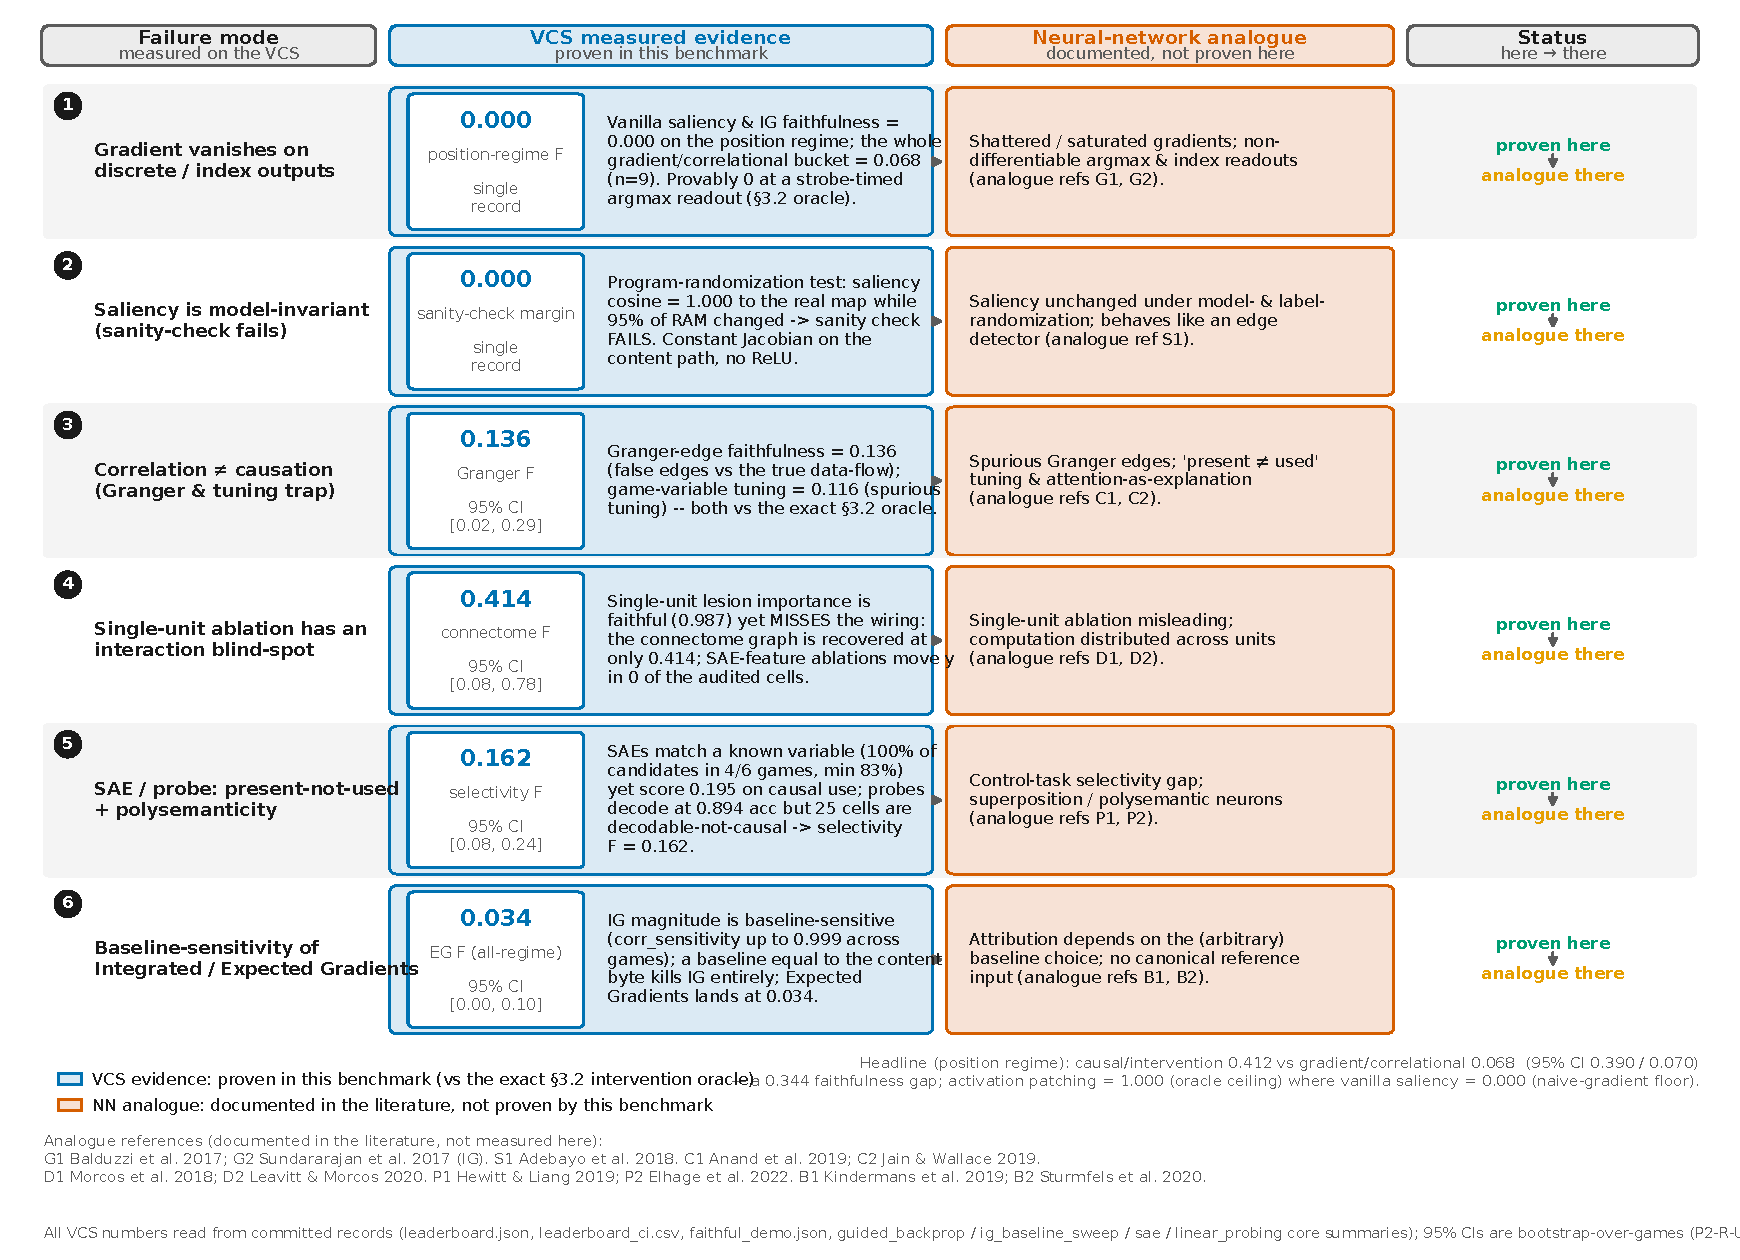
\includegraphics[width=\textwidth]{../figures/fig5_representativeness_map_full.pdf}
\caption{\textbf{Full VCS-to-NN representativeness map.} The full-density version of the
main-text map (Fig.~\ref{fig:representativeness}): each VCS failure mode is placed against its documented
neural-network analogue from the literature. The neural-network column records documented
analogues, not parallels proven by this benchmark; the oracle is the intervention oracle of
\Sectionname3.2, and the underlying per-method values trace to
\texttt{compare/out/leaderboard.json} via Sec.~\ref{supp:provenance}. Note that this full
map is the figure the simplified main-text version condenses.}
\label{supp:fig:repmap}
\end{figure}

\begin{figure}[t]
\centering
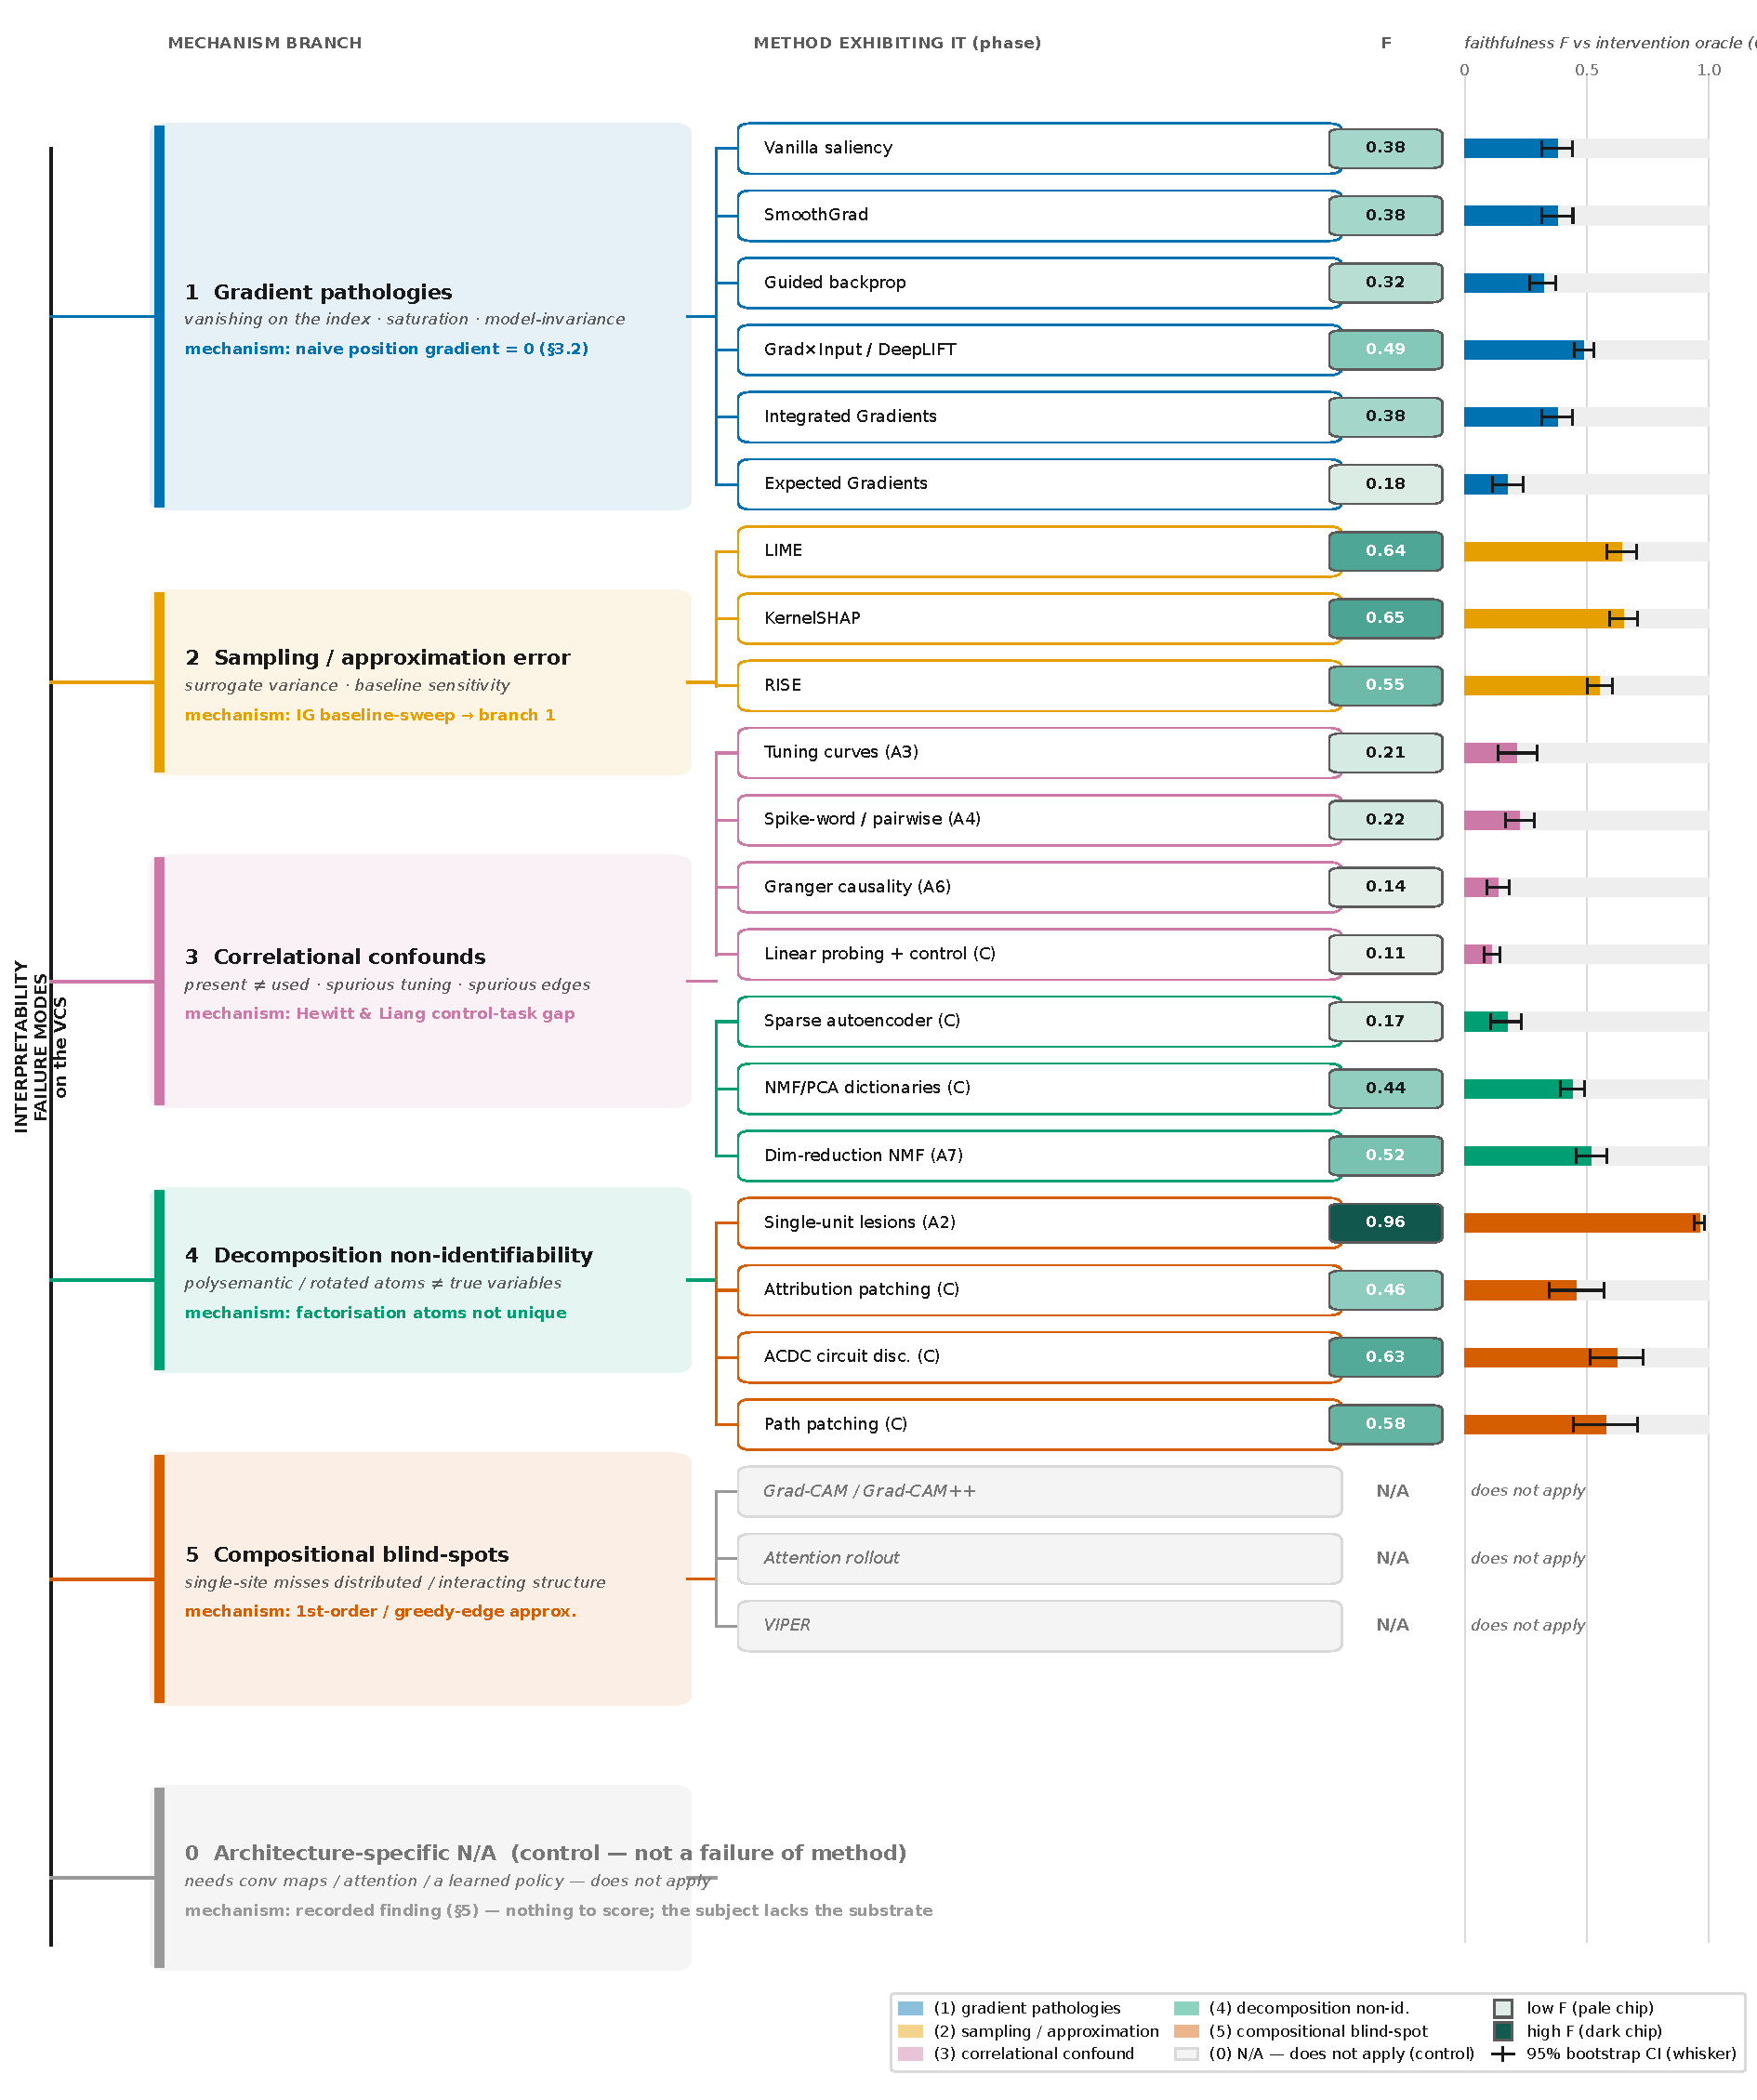
\includegraphics[width=\textwidth]{../figures/fig6_failure_taxonomy_full.pdf}
\caption{\textbf{Full failure taxonomy.} The full-density version of the main-text taxonomy
(Fig.~\ref{fig:taxonomy}): the families of interpretability failure observed on the machine, each annotated
with its faithfulness against the intervention oracle (\Sectionname3.2), reported as $F$ with its
$95\%$ bootstrap confidence interval. The leaf values trace to
\texttt{compare/out/leaderboard.json} and \texttt{leaderboard\_ci.csv} via
Sec.~\ref{supp:provenance}. Note that the gradient and correlational branches collapse on
the discrete position regime, where the naive gradient is provably zero (Prop.~\ref{prop:zero}).}
\label{supp:fig:taxonomy}
\end{figure}

\section{Plausibility-proxy rubric and its sensitivity}\label{supp:plausibility}

The plausibility axis of the leaderboard is a documented, tradition-level proxy, not a
human-subjects measurement. This section records how each value was assigned. It also shows
that the headline contrast does not depend on the particular numbers chosen. The Methods
(\Sectionname\ref{sec:triad}) name two reporting axes. Faithfulness is measured on the machine against the
intervention oracle of \Sectionname\ref{sec:oracle}. The plausibility proxy stands in for how convincing a
tradition's explanations are usually taken to be. We assign the proxy once per method
tradition, before any faithfulness score on our machine is computed, so it cannot be tuned to
the result. Its only job is to expose the danger zone of explanations that look convincing yet
are unfaithful. For that job it must be coarse, fixed in advance, and sourced rather than
precise.

The rubric assigns one proxy per tradition on a fixed five-step scale. It scores two
documented properties of each tradition's typical output and takes their average. The first
property is whether the explanation produces a dense, picture-like artifact that a reader sees
as an account of the computation. Heatmaps and saliency-style maps over the input are read as
convincing by construction. This is the perceptual-immediacy axis. The second property is
whether the field has historically treated the tradition's output as a self-evident
explanation rather than a hypothesis to be tested. This is the adoption-as-explanation axis. A
tradition that scores high on both, such as gradient saliency, receives a high proxy. A
tradition whose output is an austere intervention table or a circuit edge list, rarely
mistaken for a finished story, receives a low one. The scale is deliberately blunt,
$\{0.3,0.5,0.55,0.75,0.8,0.85,0.9\}$. A proxy meant to expose a danger zone gains nothing from
false precision, and a finer scale would invite over-reading. Every value in
Table~\ref{supp:tab:plausrubric} traces to the \jkey{plausibility_proxy} field of the
per-method rows in \texttt{compare/out/leaderboard.json}. The table only groups those rows by
tradition and records the rationale.

\begin{table}[t]
\centering
\caption{\textbf{Plausibility-proxy rubric.} The proxy assigned to each method tradition,
with the documented rationale. Values are the \jkey{plausibility_proxy} field of the
leaderboard rows (\texttt{compare/out/leaderboard.json}). They are tradition-level and fixed
before any faithfulness score is computed, so the proxy cannot be tuned to the measured
faithfulness. A higher value means an explanation that the field tends to find more
convincing, not one that is more faithful. The oracle (\Sectionname\ref{sec:oracle}) is the positive control and
is not a method under test.}
\label{supp:tab:plausrubric}
\begin{tabular}{@{}llp{6.4cm}@{}}
\toprule
Tradition & Proxy & Rationale (documented basis) \\
\midrule
gradient        & $0.90$ & Dense input-space heatmaps read as a visual account of the
                            decision; the most widely adopted XAI outputs, routinely shown
                            as if self-explanatory. \\
probing         & $0.85$ & A trained decoder that ``finds'' a concept reads as evidence the
                            concept is used; high adoption, though decodability is not
                            causal use. \\
correlational   & $0.80$ & Tuning curves and coupling spectra match the neuroscience idiom
                            of a convincing single-unit account. \\
dim.\ reduction & $0.75$ & Low-dimensional factors and dictionary atoms look like a clean
                            summary of the representation. \\
intervention    & $0.55$ & Occlusion and counterfactual outputs are quantitative tables, less
                            immediately picture-like, treated as tests rather than stories. \\
causal          & $0.50$ & Circuit edge lists and patching results are austere artifacts
                            rarely mistaken for a finished narrative. \\
descriptive     & $0.30$ & Whole-state recording is an explicit non-explanation: it withholds
                            nothing and reads as a dump, not an account. \\
\midrule
oracle (control)& $1.00$ & The \Sectionname\ref{sec:oracle} ground truth by construction; positive control, not a
                            method under test. \\
\bottomrule
\end{tabular}
\end{table}

The paper draws a contrast between this proxy and measured faithfulness. On the committed
records the two move in opposite directions. Across the thirty methods under test the Spearman
rank correlation between faithfulness and the proxy is $-0.36$, a negative association.
The traditions the field finds most convincing are, on this machine, among the least faithful.
Eight methods fall in the danger zone, defined here as a proxy of at least $0.70$ together
with a faithfulness below $0.40$. They include the correlational neuroscience methods, Expected
Gradients, guided backprop, linear probing, and the sparse autoencoder. The per-method extreme
makes the point sharply. Vanilla saliency has the highest proxy, $0.9$, yet scores faithfulness
$0.115$ on the position regime. Activation patching has a lower proxy, $0.5$, and scores $1.0$.
Here the less faithful method is the more plausible one. These figures are produced by
\texttt{tools/xai\_study/compare/plausibility\_sensitivity.py} from the leaderboard and
recorded in \texttt{compare/out/plausibility\_sensitivity.csv}.

A proxy fixed by a coarse rubric raises the question of whether the contrast is an artifact of
the particular numbers. The answer is that it is not. We perturb the proxy under four
deterministic schemes and recompute the relationship each time. The analysis uses fixed,
index-keyed offsets rather than random draws, so it re-derives bit-for-bit. The first scheme
adds a fixed per-method jitter of magnitude $\sigma\in\{0.05,0.1,0.2\}$, alternating in sign by
row. The second compresses every proxy toward the common mean by a fraction $\sigma$, which
preserves the rank order of traditions. The third uses the same index-keyed offsets at
$\sigma\in\{0.1,0.2\}$, large enough to swap neighbouring traditions' ranks. The fourth drops
one whole tradition at a time and recomputes on the remainder. Across all fourteen
perturbations the rank correlation between faithfulness and proxy stays negative. It ranges
from $-0.76$ to $-0.08$. The danger zone stays populated, with
between four and ten methods. The per-method anchor sign holds in every scheme where both
anchor methods are present, the more plausible saliency remaining the less faithful. Two runs
bound the range. The strongest is the leave-the-gradient-tradition-out run. It removes the most
plausible and least faithful block at once, and still leaves six danger-zone methods and a rank
correlation of $-0.76$. The weakest is the leave-the-causal-tradition-out run, where the
correlation falls to $-0.08$, close to zero; removing the faithful causal block flattens the
association, so the contrast is carried in part by that block. Table~\ref{supp:tab:plaussens}
reports the full sweep. The contrast keeps its sign under every alternative proxy assignment we
tried: plausibility and faithfulness are not the same axis, and high plausibility is no
guarantee of faithfulness.

\begin{table}[t]
\centering
\caption{\textbf{Proxy-sensitivity sweep.} The faithfulness-versus-proxy relationship under
each perturbation, from \texttt{compare/out/plausibility\_sensitivity.csv}. ``$\rho$'' is the
Spearman rank correlation between faithfulness and proxy over the methods present. ``danger''
is the count of high-proxy ($\geq0.70$), low-faithfulness ($<0.40$) methods. ``anchor'' is
$1$ when the more plausible saliency is the less faithful of the saliency/activation-patching
pair, and blank where a leave-one-out run removes an anchor. The baseline rubric is the first
row. Across every scheme the correlation stays negative and the danger zone stays populated.}
\label{supp:tab:plaussens}
\begin{tabular}{@{}llrrrc@{}}
\toprule
Scheme & Param & $n$ & $\rho$ & Danger & Anchor \\
\midrule
baseline                & ---           & 30 & $-0.36$ &  8 & 1 \\
additive jitter         & $\sigma=0.05$ & 30 & $-0.40$ &  8 & 1 \\
additive jitter         & $\sigma=0.10$ & 30 & $-0.41$ &  8 & 1 \\
additive jitter         & $\sigma=0.20$ & 30 & $-0.42$ & 10 & 1 \\
rank-preserving         & $\sigma=0.10$ & 30 & $-0.36$ &  8 & 1 \\
rank-preserving         & $\sigma=0.20$ & 30 & $-0.36$ &  8 & 1 \\
rank-jittering          & $\sigma=0.10$ & 30 & $-0.41$ &  8 & 1 \\
rank-jittering          & $\sigma=0.20$ & 30 & $-0.42$ & 10 & 1 \\
leave-out causal        & ---           & 24 & $-0.08$ &  8 & \\
leave-out correlational & ---           & 26 & $-0.40$ &  4 & 1 \\
leave-out descriptive   & ---           & 29 & $-0.29$ &  8 & 1 \\
leave-out dim.\ red.    & ---           & 27 & $-0.34$ &  7 & 1 \\
leave-out gradient      & ---           & 20 & $-0.76$ &  6 & \\
leave-out intervention  & ---           & 25 & $-0.34$ &  8 & 1 \\
leave-out probing       & ---           & 29 & $-0.36$ &  7 & 1 \\
\bottomrule
\end{tabular}
\end{table}

 into main.tex). It is also
%% a self-contained \input target: the six S-files below carry all SI content the main
%% paper promises (improvement_instructions P0#2, P0#4; P1#13, P1#14, P1#21; P3#35, P3#36).
%%
%% It re-uses, but does not re-derive, the §3 F/S/M definitions (S03 is authoritative)
%% and the canonical method count "30 interpretability methods + the oracle positive
%% control = 31 rows" (S07 is authoritative). Every reported number traces to a committed
%% record under tools/xai_study/compare/out/ (verifiable via the §6.5 traceability table
%% of REPRODUCIBILITY.md and re-derived by S5 below).
%%
%% Standalone compile (for review, before R6 wires it into main): wrap this file in the
%% sn-jnl preamble of a scratch driver (\documentclass[sn-nature,pdflatex]{sn-jnl} +
%% graphicx, booktabs, multirow, amsmath, longtable) and %% supplement.tex — Supplementary Information for Paper 2 (xai_2_interpretability).
%%
%% SCRUM note (P2-R-SUPP): this fragment is \input{} into the main paper by the SM
%% integration write (R6 wires %% supplement.tex — Supplementary Information for Paper 2 (xai_2_interpretability).
%%
%% SCRUM note (P2-R-SUPP): this fragment is \input{} into the main paper by the SM
%% integration write (R6 wires \input{supplement/supplement} into main.tex). It is also
%% a self-contained \input target: the six S-files below carry all SI content the main
%% paper promises (improvement_instructions P0#2, P0#4; P1#13, P1#14, P1#21; P3#35, P3#36).
%%
%% It re-uses, but does not re-derive, the §3 F/S/M definitions (S03 is authoritative)
%% and the canonical method count "30 interpretability methods + the oracle positive
%% control = 31 rows" (S07 is authoritative). Every reported number traces to a committed
%% record under tools/xai_study/compare/out/ (verifiable via the §6.5 traceability table
%% of REPRODUCIBILITY.md and re-derived by S5 below).
%%
%% Standalone compile (for review, before R6 wires it into main): wrap this file in the
%% sn-jnl preamble of a scratch driver (\documentclass[sn-nature,pdflatex]{sn-jnl} +
%% graphicx, booktabs, multirow, amsmath, longtable) and \input{supplement}; the tables
%% render without overfull boxes and the two SI figures resolve from ../figures/.

\clearpage
\appendix

%% Breakable monospaced JSON key: lets long under_scored keys wrap inside narrow table
%% columns. Used by S5 (number provenance). Defined here so the S-files stay self-contained.
\providecommand{\jkey}[1]{\texttt{\expandafter\jkeyaux#1\relax}}
\makeatletter
\def\jkeyaux#1{\ifx\relax#1\else
  \ifx_#1\discretionary{}{}{}\char`\_\else
    \ifx.#1\discretionary{}{}{}.\else#1\fi\fi
  \expandafter\jkeyaux\fi}
\makeatother

\section*{Supplementary Information}
\setcounter{table}{0}
\setcounter{figure}{0}
\renewcommand{\thetable}{S\arabic{table}}
\renewcommand{\thefigure}{S\arabic{figure}}
\renewcommand{\thesection}{S\arabic{section}}
\setcounter{section}{0}

This Supplementary Information records what the main paper summarizes. We give the
per-method protocols (\Sectionname\ref{supp:protocols}) and the leaderboard schema with its glossary
(\Sectionname\ref{supp:schema}). We give the coverage and applicability of every method across games
and output regimes (\Sectionname\ref{supp:coverage}). We map each headline claim to its evidence
(\Sectionname\ref{supp:claims}). We trace the provenance of every headline number down to the record
file and command that produced it (\Sectionname\ref{supp:provenance}). We state plainly what the
paper does not claim (\Sectionname\ref{supp:notclaimed}). We give the plausibility-proxy rubric and
its sensitivity analysis (\Sectionname\ref{supp:plausibility}). The main text shows simplified forms
of two diagnostic figures; we reproduce both here at full resolution
(Figs.~\ref{supp:fig:repmap} and~\ref{supp:fig:taxonomy}).
The correctness triad $\mathrm{F}\wedge\mathrm{S}\wedge\mathrm{M}$ used throughout is the
one defined in the main Methods (\Sectionname\ref{sec:triad}); we reference it here rather than restating it. The
benchmark scores 30 interpretability methods together with the intervention oracle (\Sectionname\ref{sec:oracle})
as a positive control, for 31 leaderboard rows in total.

\input{supplement/S1_per_method_protocols}
\input{supplement/S2_benchmark_schema}
\input{supplement/S3_coverage_applicability}
\input{supplement/S4_claims_evidence}
\input{supplement/S5_number_provenance}
\input{supplement/S6_not_claimed}
\input{supplement/S7_plausibility}
 into main.tex). It is also
%% a self-contained \input target: the six S-files below carry all SI content the main
%% paper promises (improvement_instructions P0#2, P0#4; P1#13, P1#14, P1#21; P3#35, P3#36).
%%
%% It re-uses, but does not re-derive, the §3 F/S/M definitions (S03 is authoritative)
%% and the canonical method count "30 interpretability methods + the oracle positive
%% control = 31 rows" (S07 is authoritative). Every reported number traces to a committed
%% record under tools/xai_study/compare/out/ (verifiable via the §6.5 traceability table
%% of REPRODUCIBILITY.md and re-derived by S5 below).
%%
%% Standalone compile (for review, before R6 wires it into main): wrap this file in the
%% sn-jnl preamble of a scratch driver (\documentclass[sn-nature,pdflatex]{sn-jnl} +
%% graphicx, booktabs, multirow, amsmath, longtable) and %% supplement.tex — Supplementary Information for Paper 2 (xai_2_interpretability).
%%
%% SCRUM note (P2-R-SUPP): this fragment is \input{} into the main paper by the SM
%% integration write (R6 wires \input{supplement/supplement} into main.tex). It is also
%% a self-contained \input target: the six S-files below carry all SI content the main
%% paper promises (improvement_instructions P0#2, P0#4; P1#13, P1#14, P1#21; P3#35, P3#36).
%%
%% It re-uses, but does not re-derive, the §3 F/S/M definitions (S03 is authoritative)
%% and the canonical method count "30 interpretability methods + the oracle positive
%% control = 31 rows" (S07 is authoritative). Every reported number traces to a committed
%% record under tools/xai_study/compare/out/ (verifiable via the §6.5 traceability table
%% of REPRODUCIBILITY.md and re-derived by S5 below).
%%
%% Standalone compile (for review, before R6 wires it into main): wrap this file in the
%% sn-jnl preamble of a scratch driver (\documentclass[sn-nature,pdflatex]{sn-jnl} +
%% graphicx, booktabs, multirow, amsmath, longtable) and \input{supplement}; the tables
%% render without overfull boxes and the two SI figures resolve from ../figures/.

\clearpage
\appendix

%% Breakable monospaced JSON key: lets long under_scored keys wrap inside narrow table
%% columns. Used by S5 (number provenance). Defined here so the S-files stay self-contained.
\providecommand{\jkey}[1]{\texttt{\expandafter\jkeyaux#1\relax}}
\makeatletter
\def\jkeyaux#1{\ifx\relax#1\else
  \ifx_#1\discretionary{}{}{}\char`\_\else
    \ifx.#1\discretionary{}{}{}.\else#1\fi\fi
  \expandafter\jkeyaux\fi}
\makeatother

\section*{Supplementary Information}
\setcounter{table}{0}
\setcounter{figure}{0}
\renewcommand{\thetable}{S\arabic{table}}
\renewcommand{\thefigure}{S\arabic{figure}}
\renewcommand{\thesection}{S\arabic{section}}
\setcounter{section}{0}

This Supplementary Information records what the main paper summarizes. We give the
per-method protocols (\Sectionname\ref{supp:protocols}) and the leaderboard schema with its glossary
(\Sectionname\ref{supp:schema}). We give the coverage and applicability of every method across games
and output regimes (\Sectionname\ref{supp:coverage}). We map each headline claim to its evidence
(\Sectionname\ref{supp:claims}). We trace the provenance of every headline number down to the record
file and command that produced it (\Sectionname\ref{supp:provenance}). We state plainly what the
paper does not claim (\Sectionname\ref{supp:notclaimed}). We give the plausibility-proxy rubric and
its sensitivity analysis (\Sectionname\ref{supp:plausibility}). The main text shows simplified forms
of two diagnostic figures; we reproduce both here at full resolution
(Figs.~\ref{supp:fig:repmap} and~\ref{supp:fig:taxonomy}).
The correctness triad $\mathrm{F}\wedge\mathrm{S}\wedge\mathrm{M}$ used throughout is the
one defined in the main Methods (\Sectionname\ref{sec:triad}); we reference it here rather than restating it. The
benchmark scores 30 interpretability methods together with the intervention oracle (\Sectionname\ref{sec:oracle})
as a positive control, for 31 leaderboard rows in total.

\input{supplement/S1_per_method_protocols}
\input{supplement/S2_benchmark_schema}
\input{supplement/S3_coverage_applicability}
\input{supplement/S4_claims_evidence}
\input{supplement/S5_number_provenance}
\input{supplement/S6_not_claimed}
\input{supplement/S7_plausibility}
; the tables
%% render without overfull boxes and the two SI figures resolve from ../figures/.

\clearpage
\appendix

%% Breakable monospaced JSON key: lets long under_scored keys wrap inside narrow table
%% columns. Used by S5 (number provenance). Defined here so the S-files stay self-contained.
\providecommand{\jkey}[1]{\texttt{\expandafter\jkeyaux#1\relax}}
\makeatletter
\def\jkeyaux#1{\ifx\relax#1\else
  \ifx_#1\discretionary{}{}{}\char`\_\else
    \ifx.#1\discretionary{}{}{}.\else#1\fi\fi
  \expandafter\jkeyaux\fi}
\makeatother

\section*{Supplementary Information}
\setcounter{table}{0}
\setcounter{figure}{0}
\renewcommand{\thetable}{S\arabic{table}}
\renewcommand{\thefigure}{S\arabic{figure}}
\renewcommand{\thesection}{S\arabic{section}}
\setcounter{section}{0}

This Supplementary Information records what the main paper summarizes. We give the
per-method protocols (\Sectionname\ref{supp:protocols}) and the leaderboard schema with its glossary
(\Sectionname\ref{supp:schema}). We give the coverage and applicability of every method across games
and output regimes (\Sectionname\ref{supp:coverage}). We map each headline claim to its evidence
(\Sectionname\ref{supp:claims}). We trace the provenance of every headline number down to the record
file and command that produced it (\Sectionname\ref{supp:provenance}). We state plainly what the
paper does not claim (\Sectionname\ref{supp:notclaimed}). We give the plausibility-proxy rubric and
its sensitivity analysis (\Sectionname\ref{supp:plausibility}). The main text shows simplified forms
of two diagnostic figures; we reproduce both here at full resolution
(Figs.~\ref{supp:fig:repmap} and~\ref{supp:fig:taxonomy}).
The correctness triad $\mathrm{F}\wedge\mathrm{S}\wedge\mathrm{M}$ used throughout is the
one defined in the main Methods (\Sectionname\ref{sec:triad}); we reference it here rather than restating it. The
benchmark scores 30 interpretability methods together with the intervention oracle (\Sectionname\ref{sec:oracle})
as a positive control, for 31 leaderboard rows in total.

\section{Per-method protocols}\label{supp:protocols}

This section records five things for each method under test. It records the exact objects the
method consumes and produces, the reference it is scored against, its sampling or optimization
budget, the metric that turns its output into a faithfulness score, and the committed record
file (version-controlled, in the released repository) that holds the per-game results. All methods share one evaluation contract. We state that
contract once and then specialize it per method. Every method receives the same bit-exact VCS
state on each game of the scored set. We state the contract on the six core games
(\texttt{breakout}, \texttt{ms\_pacman}, \texttt{pong}, \texttt{qbert}, \texttt{seaquest},
\texttt{space\_invaders}), which carry the full tiered ground truth and the exact oracle and
serve as the running example; the aggregate leaderboard scores extend the identical protocol
to the 42-game scored set of \Sectionname\ref{supp:scoredset}. That state is not the boot screen.
It is a shared gameplay state, produced by a single seeded random-action stream (seed~$0$) run
for a $90$-frame prefix and then rolled forward for a $15$-frame analysis horizon. The stream is
deterministic, so every method sees the identical state on each game, and the run is asserted
bit-exact per game. An oracle cause-density gate screens the state before any method runs. The
gate counts how many candidate causes move the output above a floor and rejects states with too
few, so a near-flat oracle column cannot pass. This gate is what turns a degenerate frame into a
usable one; on \texttt{seaquest} it raises the count of live candidate causes from $2$ to $19$.
The candidate-cause set is the machine's own state. This set is the RAM bytes together with the
CPU registers and the TIA and RIOT registers exposed by the substrate. The output every method
attributes over is a shared screen-buffer region read at the end of the analysis horizon, not a
single hand-picked pixel. The reference is the intervention oracle of \Sectionname\ref{sec:oracle},
evaluated by exact re-runs of the emulator under $\mathrm{do}(u)$. A method that
cannot be applied to a given output regime is recorded as not-applicable rather than scored
as zero. An empty result is therefore never read as a wrong one. Faithfulness is the F
axis of the main-text triad (\Sectionname\ref{sec:triad}); we reference that definition and do not restate it.
Records live under \texttt{tools/xai\_study/<phase>/out/}; the aggregate they feed is
\texttt{tools/xai\_study/compare/out/leaderboard.json}.
Table~\ref{supp:leaderboard} consolidates the triad scores for all thirty methods and the
oracle positive control in one place; the per-method protocols follow.

\begin{table*}[t]
\centering
\caption{\textbf{Consolidated leaderboard: all methods, all triad axes.} One row per method
across the three phases, plus the intervention oracle as a positive control. $F$ is
faithfulness (Pearson correlation against the oracle, with the bootstrap-over-games 95\% CI in
brackets), $S$ is sufficiency, $M$ is minimality, all as defined in \Sectionname\ref{sec:triad};
Plaus is the elicited plausibility prior and $n$ is the number of scored games. Attribution
methods that emit only a saliency have no defined $S$ or $M$ and are marked ``---''; A5
(field potentials) and A7 (dimensionality reduction) likewise lack the $S$/$M$ decomposition.
Values are transcribed from \texttt{tools/xai\_study/compare/out/leaderboard.json} (the
committed numbers of record).}
\label{supp:leaderboard}
\footnotesize
\setlength{\tabcolsep}{4pt}
\begin{tabularx}{\textwidth}{@{}Xccccccc@{}}
\toprule
Method & Phase & Tradition & $F$ (95\% CI) & $S$ & $M$ & Plaus & $n$ \\
\midrule
A1 connectomics & A & intervention & 0.207 [0.130, 0.293] & 0.971 & 0.967 & 0.55 & 35 \\
A2 lesions & A & intervention & 0.965 [0.942, 0.983] & 0.591 & 1.000 & 0.55 & 42 \\
A3 tuning curves & A & correlational & 0.213 [0.136, 0.295] & 0.200 & 0.928 & 0.80 & 42 \\
A4 spike-word / pairwise & A & correlational & 0.225 [0.166, 0.283] & 0.133 & 0.363 & 0.80 & 34 \\
A5 field potentials & A & correlational & 0.376 [0.323, 0.428] & --- & --- & 0.80 & 40 \\
A6 Granger & A & correlational & 0.136 [0.091, 0.184] & 0.884 & 0.647 & 0.80 & 35 \\
A7 dim.\ reduction & A & dim.\ red. & 0.519 [0.457, 0.581] & --- & --- & 0.75 & 42 \\
A8 whole-state & A & descriptive & 1.000 [1.000, 1.000] & 1.000 & 0.075 & 0.30 & 42 \\
\midrule
Vanilla saliency & B & gradient & 0.380 [0.316, 0.445] & --- & --- & 0.90 & 42 \\
smoothgrad & B & gradient & 0.380 [0.317, 0.445] & --- & --- & 0.90 & 42 \\
Guided backprop & B & gradient & 0.322 [0.267, 0.375] & --- & --- & 0.90 & 42 \\
Grad$\times$Input / DeepLIFT & B & gradient & 0.486 [0.448, 0.526] & --- & --- & 0.90 & 42 \\
Integrated Gradients & B & gradient & 0.379 [0.314, 0.444] & --- & --- & 0.90 & 42 \\
Expected Gradients & B & gradient & 0.175 [0.110, 0.240] & --- & --- & 0.90 & 42 \\
kernelshap & B & gradient & 0.652 [0.596, 0.709] & --- & --- & 0.90 & 42 \\
lime & B & gradient & 0.644 [0.582, 0.705] & --- & --- & 0.90 & 42 \\
rise & B & gradient & 0.552 [0.500, 0.600] & --- & --- & 0.90 & 42 \\
occlusion & B & intervention & 0.687 [0.624, 0.746] & --- & --- & 0.55 & 42 \\
Extremal perturbation & B & intervention & 0.461 [0.410, 0.513] & --- & --- & 0.55 & 42 \\
On-distribution counterfactual & B & intervention & 0.433 [0.343, 0.522] & --- & --- & 0.55 & 42 \\
\midrule
Activation patching & C & causal & 1.000 [1.000, 1.000] & --- & --- & 0.50 & 42 \\
Causal scrubbing & C & causal & 0.979 [0.940, 1.000] & 0.979 & 0.814 & 0.50 & 42 \\
Interchange interventions (DAS) & C & causal & 1.000 [1.000, 1.000] & --- & --- & 0.50 & 42 \\
Logit / tuned lens & C & causal & 0.820 [0.768, 0.871] & --- & 0.224 & 0.50 & 42 \\
Path patching & C & causal & 0.580 [0.452, 0.710] & --- & --- & 0.50 & 42 \\
ACDC & C & causal & 0.625 [0.514, 0.730] & 0.299 & 1.000 & 0.50 & 35 \\
Attribution patching & C & gradient & 0.456 [0.345, 0.573] & --- & --- & 0.90 & 42 \\
Linear probing (+ control) & C & probing & 0.240 [0.153, 0.346] & --- & 0.932 & 0.85 & 42 \\
NMF / PCA dictionaries & C & dim.\ red. & 0.102 [0.049, 0.160] & 0.751 & 0.966 & 0.75 & 42 \\
Sparse autoencoder & C & dim.\ red. & 0.153 [0.096, 0.218] & 0.183 & 0.934 & 0.75 & 40 \\
\midrule
Intervention oracle & --- & oracle & 1.000 [1.000, 1.000] & 1.000 & 1.000 & 1.00 & 1 \\
\bottomrule
\end{tabularx}
\end{table*}

The neuroscience analyses (Phase~A) treat the running machine as a brain. It asks how far
each classical analysis recovers the known mechanism on the shared gameplay state. Each
method's baseline is the exact data-flow graph or causal role that the substrate makes
available. Its budget is the scored set (\Sectionname\ref{supp:scoredset}) unless noted,
with the six-game core as the running example, and its scoring metric is named in
Table~\ref{supp:tab:phaseA}. One core cell is honestly degenerate. On \texttt{ms\_pacman} the
pairwise analysis (A4) finds no coupled candidate pair to score at that frame, so its
\texttt{ms\_pacman} value is uninformative rather than a failure; the other five games carry
it.

\begin{table}[t]
\centering
\caption{\textbf{Phase~A protocols (neuroscience analyses).} One row per method. The columns
give the input it reads, the reference it is scored against, the sampling or intervention
budget, the scoring metric, and the committed record. All eight run on the scored set
(\Sectionname\ref{supp:scoredset}), with the six core games as the running example;
faithfulness is the F axis of \Sectionname\ref{sec:triad}. The whole-state recording (A8) is included as a
descriptive upper bound on coverage. Its faithfulness $F$ is trivial, so we read it for its
minimality $M$.}
\label{supp:tab:phaseA}
\scriptsize
\setlength{\tabcolsep}{4pt}
\begin{tabular}{@{}p{1.7cm}p{2.6cm}p{1.9cm}p{2.6cm}p{1.0cm}@{}}
\toprule
Method & Input / candidate causes & Reference & Scoring metric & Record \\
\midrule
A1 connectomics & RAM/register activity over trajectory & data-flow graph & data-flow graph $F_1$ vs.\ oracle & A1 \\
A2 lesions & single-cell knockouts via $\mathrm{do}(u)$ & true causal role & lesion-importance $\rho$ vs.\ role & A2 \\
A3 tuning curves & per-cell response vs.\ variable & variable coupling & $1-$ spurious-tuning rate & A3 \\
A4 spike-word / pairwise & pairwise cell correlations & true coupling & corr.\ $\rho$ vs.\ coupling & A4 \\
A5 field potentials & pooled-activity spectra & true causal share & $1-$ clock-explained var. & A5 \\
A6 Granger & directed lag structure & true data-flow & $1-$ false-edge rate & A6 \\
A7 dim.\ reduction & NMF/PCA over activity & known variables & NMF matched-component frac. & A7 \\
A8 whole-state & full state record & oracle decomp. & minimality $M$ vs.\ oracle & A8 \\
\bottomrule
\end{tabular}

\smallskip
\noindent\scriptsize Records: \texttt{tools/xai\_study/phaseA\_kording/out/A\{1..8\}\_*}; all
eight run on the 42-game scored set (\Sectionname\ref{supp:scoredset}), with the six core
games as the running example (\jkey{n_games} per method in \jkey{leaderboard.json}).
\end{table}

The attribution methods (Phase~B) run the everyday XAI toolbox over the same gameplay state.
These methods produce a real-valued saliency or attribution over the candidate-cause set.
We score that output by Pearson correlation against the oracle attribution. The gradient family
runs with the bilinear sub-pixel sampler turned on, so it is scored on a real position gradient
and not on the naive one. The naive gradient of the discrete position output is provably zero
(Prop.~\ref{prop:zero}); the sampler restores a finite gradient, but the restored gradient is
low and mixed in faithfulness rather than a fix. Expected Gradients draws its reference pool
from the states of the same seeded gameplay trajectory, not from a synthetic baseline. Two cells
are honestly degenerate and recorded as such. The on-distribution counterfactual returns a zero
delta on \texttt{space\_invaders}, \texttt{ms\_pacman}, and \texttt{qbert}, where its perturbation
does not move the shared output at that frame; those cells are marked not-valid rather than
scored. Expected Gradients scores low on the content regime of every game except \texttt{pong},
because the causal byte it should land on is static there. The budgets that matter are the
Monte-Carlo or perturbation counts of the sampling estimators, recorded per method in
Table~\ref{supp:tab:phaseB}. The seed-dispersion of the stochastic members is carried in
\texttt{leaderboard\_ci.csv} (\texttt{seed\_sd}, \texttt{seed\_sd\_source}) and reproduced
in \Sectionname\ref{supp:provenance}.

\begin{table}[t]
\centering
\caption{\textbf{Phase~B protocols (attribution methods).} Each method emits a saliency over
the candidate-cause set. We score it by Pearson correlation against the oracle attribution
(\Sectionname\ref{sec:oracle}). The reference is shared and the budget is the scored set of
\Sectionname\ref{supp:scoredset} (six core games as the running example). The budget column records the
sampling or perturbation count that drives each estimator. The seed column flags which
methods carry an independent-seed dispersion in \texttt{leaderboard\_ci.csv}.}
\label{supp:tab:phaseB}
\scriptsize
\setlength{\tabcolsep}{4pt}
\begin{tabular}{@{}p{2.9cm}p{1.75cm}p{4.3cm}p{1.15cm}@{}}
\toprule
Method & Tradition & Budget / hyperparameters & Seed sd \\
\midrule
Vanilla saliency & gradient & single backward pass & --- \\
smoothgrad & gradient & noise-averaged gradient; $\sigma$-robustness committed & 0.0 \\
Guided backprop & gradient & single guided pass & --- \\
Grad$\times$Input / DeepLIFT & gradient & DeepLIFT reference-difference & --- \\
Integrated Gradients & gradient & path integral, baseline = zero state & --- \\
Expected Gradients & gradient & expectation over baselines (refits) & yes \\
kernelshap & gradient & Monte-Carlo coalition sampling ($\propto 1/\sqrt{N}$) & 0.017 \\
lime & gradient & local linear fit, perturbation refits & 0.029 \\
rise & gradient & random-mask Monte-Carlo ($\propto 1/\sqrt{N}$) & 0.051 \\
occlusion & intervention & exhaustive single-cell masking & --- \\
Extremal perturbation & intervention & optimized mask, area-constrained & --- \\
On-distribution counterfactual & intervention & on-manifold $\mathrm{do}(u)$ resampling & --- \\
\bottomrule
\end{tabular}

\smallskip
\noindent\scriptsize Records: \texttt{tools/xai\_study/phaseB\_attribution/out/}; all twelve run
on the 42-game scored set (\Sectionname\ref{supp:scoredset}), six core games as the running
example, and are scored by Pearson correlation against the oracle (\Sectionname\ref{sec:oracle}). Seed
sd is the independent-seed dispersion from \texttt{leaderboard\_ci.csv}.
\end{table}

The mechanistic methods (Phase~C) are built to recover circuits. Each is scored
against the true data-flow or the exact recovered-minus-exact deviation. The causal members
of this phase are the ones that reach the oracle ceiling. We list their exact scoring metric
so that the ceiling is not read as a tautology. Each member is scored against the substrate's
known routine, and not against another method. Two members (NMF/PCA dictionaries and the
sparse autoencoder) are dimensionality-reduction methods carried here for comparison. The
sparse autoencoder has two aggregations that differ, which we reconcile in
\Sectionname\ref{supp:provenance}.

\begin{table}[t]
\centering
\caption{\textbf{Phase~C protocols (mechanistic methods).} Each method is scored against the
substrate's known circuit or the exact recovered-minus-exact deviation (\Sectionname\ref{sec:oracle}), and not
against another method. This is what keeps the oracle ceiling non-circular. The probing and
dictionary-learning members are included for comparison with the causal members.}
\label{supp:tab:phaseC}
\scriptsize
\setlength{\tabcolsep}{4pt}
\begin{tabular}{@{}p{3.4cm}p{1.4cm}p{5.2cm}@{}}
\toprule
Method & Tradition & Scoring metric \\
\midrule
Activation patching & causal & $\max|\text{recovered}-\text{exact}|$ vs.\ oracle \\
Causal scrubbing & causal & scrubbing-preserved performance \\
Interchange interventions (DAS) & causal & aligned interchange accuracy \\
Logit / tuned lens & causal & logit-lens fidelity to true intermediate \\
Path patching & causal & path-circuit $F_1$ vs.\ true routine \\
ACDC & causal & discovered-circuit best $F_1$ vs.\ data-flow \\
Attribution patching & gradient & corr.\ of approximation vs.\ exact patch \\
Linear probing (+ control) & probing & selectivity vs.\ control task \\
NMF / PCA dictionaries & dim.\ red. & matched-component fraction vs.\ vars \\
Sparse autoencoder & dim.\ red. & feature-variable matched fraction \\
\bottomrule
\end{tabular}

\smallskip
\noindent\scriptsize Records: \texttt{tools/xai\_study/phaseC\_mechanistic/out/}; all ten run
on the 42-game scored set (\Sectionname\ref{supp:scoredset}), with the six core games as the
running example.
\end{table}

The intervention oracle is the positive control, not a method under test. It is the exact
$\mathrm{do}(u)$ ground truth of \Sectionname\ref{sec:oracle}, evaluated by re-running the bit-exact machine. It
attains $F=S=M=1.0$ by construction. Its record triple is the intervention oracle, the
content-path gradient oracle, and their cross-check
(\texttt{tools/xai\_study/ground\_truth/out/}). It anchors the ceiling against which every
other row is read, which is why it occupies the thirty-first leaderboard row.

\section{Benchmark schema and glossary}\label{supp:schema}

The leaderboard is built from a flat record schema. Stating it removes the ambiguity
about what a single number on the benchmark counts. Each method is run per game and writes a
per-game record under its phase's \texttt{out/} tree. The leaderboard aggregates those
records into one row per method by averaging over games. The schema columns of a leaderboard
row are given in Table~\ref{supp:tab:schema}. The aggregation rule is a mean over the
$n_{\text{games}}$ games. When a method emits several output records on one game, those records
are first reduced within that game. The faithfulness, sufficiency, and minimality columns
report the F, S, and M axes defined in \Sectionname\ref{sec:triad}. We do not re-derive those definitions here.

\begin{table}[t]
\centering
\caption{\textbf{Leaderboard row schema.} The columns of one row in
\texttt{compare/out/leaderboard.json} (\texttt{rows[\,]}) and its uncertainty companion
\texttt{leaderboard\_ci.csv}. The metric column names the per-method scoring function from
\Sectionname\ref{supp:protocols}; F, S, and M are the triad axes of \Sectionname\ref{sec:triad}. Aggregation is a mean
over $n_{\text{games}}$, with bootstrap confidence intervals over games (and, where present,
over records).}
\label{supp:tab:schema}
\footnotesize
\begin{tabular}{@{}p{3.0cm}p{8.4cm}@{}}
\toprule
Column & Meaning \\
\midrule
\texttt{phase} & phaseA\_kording, phaseB\_attribution, phaseC\_mechanistic, or ground\_truth \\
\texttt{method} & method identifier (the row key) \\
\texttt{tradition} & intervention, causal, gradient, correlational, \jkey{dim_reduction}, probing, descriptive, oracle \\
\jkey{n_games} & number of games the method was scored on (up to 42 for the scored set of \Sectionname\ref{supp:scoredset}; 1 for the oracle) \\
\jkey{n_records} & number of per-game output records aggregated into the row \\
\texttt{faithfulness} (F) & faithfulness vs.\ the intervention oracle (\Sectionname\ref{sec:oracle}), $[0,1]$, higher better \\
\jkey{faithfulness_ci95} & $95\%$ bootstrap CI half-width over games \\
\jkey{faithfulness_position_regime} & F restricted to the discrete sprite-position/index regime \\
\jkey{faithfulness_content_regime} & F restricted to the continuous content regime \\
\texttt{triad\_S} / \texttt{triad\_M} & sufficiency / minimality axes (\Sectionname\ref{sec:triad}), where applicable \\
\jkey{plausibility_proxy} & documented method-tradition proxy, $[0,1]$ --- not a human-subjects measurement \\
\jkey{is_positive_control} & 1 for the oracle row, 0 otherwise \\
\jkey{metric_names} & the per-method scoring function (\Sectionname\ref{supp:protocols}) \\
\texttt{commits} & the commit(s) at which the per-game records were produced \\
\bottomrule
\end{tabular}
\end{table}

We fix the vocabulary that the schema implies, because the review asked for a single
unambiguous method count. A \emph{method} is one interpretability technique, e.g.\
\texttt{vanilla\_saliency}. A \emph{method row} is its single aggregated line on the
leaderboard. A \emph{per-game record} is one method scored on one game, written under a phase
\texttt{out/} tree. An \emph{output record} is a per-game record for one output regime; a
method may emit several of these on one game. A \emph{family mean} is the average over the
members of a tradition family, e.g.\ causal/intervention. The \emph{oracle positive control}
is the exact $\mathrm{do}(u)$ ground truth of \Sectionname\ref{sec:oracle}, scored as a method to anchor the
ceiling. A \emph{not-applicable method} is one that does not apply to a given output regime;
it is recorded as N/A rather than as a zero. With this vocabulary the count is unambiguous.
The benchmark scores 30 interpretability methods together with the intervention
oracle as a positive control, for 31 leaderboard rows in total
(\texttt{leaderboard.json.n\_methods}~$=31$), aggregating 1773 per-game records over the
42-game scored set (\texttt{n\_per\_game\_records\_aggregated}~$=1773$): 8 methods in
Phase~A, 12 in Phase~B, 10 in Phase~C, and the one oracle row. This count is the canonical one
used in the abstract, the figures, and throughout this Supplement.

\section{Coverage and applicability}\label{supp:coverage}

The benchmark scores methods on a six-game core drawn from a larger bit-exact substrate. The
coverage table makes the scope of that choice explicit. Paper~1 validates the
differentiable VCS ports bit-for-bit against the \texttt{xitari} reference on all 64 Arcade
Learning Environment games, within a 30-frame RAM and 60-frame screen window. The
interpretability study reported here runs on the six games listed in
Table~\ref{supp:tab:coverage}. Every method is scored on a shared gameplay state, produced by
one seeded random-action stream (seed~$0$, $90$-frame prefix, $15$-frame analysis horizon), not
on the boot screen. This keeps the analysis inside the Paper~1 bit-exact window while giving the
oracle a rich, non-degenerate cause set to score against. We pick these six games because all
three tiers of ground truth (\Sectionname\ref{sec:tiers}) are available for them and the oracle is
exact. The remaining 58 games are
bit-exact substrate but are not scored here. Some fall outside the validated horizon for the
analyses we run. For others, the tiered labels they would need are not yet produced. They are
candidates for the larger sweep, and are not excluded for any methodological reason. The
horizon column records the validated window. The tier column records which of the three
ground-truth tiers (T1 exact intervention, T2 data-flow, T3 externally-supplied semantic
labels) is available.

\begin{table}[t]
\centering
\caption{\textbf{Core-game coverage.} The six core games carry exact tiered ground truth and
the full method battery. Faithfulness is scored within the Paper~1 bit-exact window. The
last two columns give the methods run and the per-game output records contributed. The wider
64-game substrate is bit-exact (Paper~1) but is reserved for the larger sweep. T3 labels are
external (\Sectionname\ref{sec:tiers}); we record this so the benchmark does not appear to certify them.}
\label{supp:tab:coverage}
\footnotesize
\setlength{\tabcolsep}{4pt}
\begin{tabular}{@{}p{2.4cm}p{1.9cm}p{1.5cm}p{1.7cm}p{1.5cm}p{1.4cm}@{}}
\toprule
Game & Paper-1 status & Horizon & Tiers & Methods run & Records \\
\midrule
breakout & bit-exact & 30/60 fr & T1,T2,T3 & 30 + oracle & per-game \\
ms\_pacman & bit-exact & 30/60 fr & T1,T2,T3 & 30 + oracle & per-game \\
pong & bit-exact & 30/60 fr & T1,T2,T3 & 30 + oracle & per-game \\
qbert & bit-exact & 30/60 fr & T1,T2,T3 & 30 + oracle & per-game \\
seaquest & bit-exact & 30/60 fr & T1,T2,T3 & 30 + oracle & per-game \\
space\_invaders & bit-exact & 30/60 fr & T1,T2,T3 & 30 + oracle & per-game \\
\midrule
58 further games & bit-exact (P1) & 30/60 fr & T1,T2 partial & reserved & --- \\
\bottomrule
\end{tabular}
\end{table}

A gameplay state can still be degenerate for a particular method, and the benchmark records
this rather than scoring it as a failure. The oracle cause-density gate is the first guard. It
counts how many candidate causes move the shared output above a floor, and rejects a state that
does not clear a minimum count, so a near-flat oracle column never reaches a method. On
\texttt{seaquest} the gate raises the count of live candidate causes at the analysis frame from
$2$ to $19$, which is what makes the game usable. Three residual degenerate cells survive the
gate and are marked, not scored as zero. On \texttt{ms\_pacman} the pairwise neuroscience
analysis (A4) finds no coupled candidate pair at that frame, so its cell is uninformative. The
on-distribution counterfactual returns a zero delta on \texttt{space\_invaders},
\texttt{ms\_pacman}, and \texttt{qbert}, where its perturbation does not move the shared output;
those cells are recorded as not-valid. Expected Gradients scores low on the content regime of
every game but \texttt{pong}, because the causal byte it should attribute to is static there.
None of these cells is read as a wrong answer.

Whether a method applies at all depends on what the method needs from its target. The
applicability matrix records that for every method family. The Phase~A neuroscience analyses
read the raw machine state and need neither a learned policy nor gradients. The Phase~B
attribution methods split into two groups. The gradient members need a differentiable forward
pass. The intervention members need only the ability to set state. The Phase~C mechanistic
methods need access to internal activations. The causal members among them also need the
ability to intervene. Table~\ref{supp:tab:applic} records, per family, whether the method
operates on the raw VCS, whether it requires a learned policy, gradients, internal layers or
attention, or external labels, whether it uses oracle-like interventions, and whether it
receives a supplied hypothesis. The table shows the same pattern the results confirm. The
families that score high on faithfulness are the ones that can intervene. The families that
collapse on the position regime are the gradient and correlational ones.

\begin{table}[t]
\centering
\caption{\textbf{Per-family applicability.} What each method family requires of its target.
``Intervenes'' marks oracle-like $\mathrm{do}(u)$ access; ``hypothesis'' marks methods that
receive a supplied circuit hypothesis to test. The raw-VCS column distinguishes analyses that
read machine state directly from those that need a differentiable or layered model. A blank
means the requirement does not apply.}
\label{supp:tab:applic}
\footnotesize
\begin{tabular}{@{}p{3.0cm}cccccc@{}}
\toprule
Family & raw VCS & policy & gradients & layers/attn & intervenes & hypothesis \\
\midrule
A neuroscience & yes & no & no & no & A2 only & no \\
B gradient & yes & no & yes & no & no & no \\
B intervention & yes & no & no & no & yes & no \\
C causal & yes & no & no & yes & yes & yes \\
C gradient (attr.\ patch) & yes & no & yes & yes & approx. & yes \\
C probing & yes & no & no & yes & no & no \\
C / A dim.\ reduction & yes & no & no & yes & no & no \\
oracle (control) & yes & no & no & yes & exact & --- \\
\bottomrule
\end{tabular}
\end{table}

\section{Claims and evidence}\label{supp:claims}

Every headline claim in the paper rests on a specific artifact. The table in this section
makes that dependency checkable. For each claim we list the figure or table that supports it,
the games and methods it uses, the metric, the artifact it traces to, and the limitation that
bounds it. Faithfulness, sufficiency, and minimality are the three axes of \Sectionname\ref{sec:triad}.
The numbers themselves are sourced in \Sectionname\ref{supp:provenance}. The table below names which
evidence supports which claim; it does not repeat the values. One split matters for how the
table is read. The all-regime faithfulness gap between causal/intervention and
gradient/correlational methods is $0.297$ with a $95\%$ interval of $[0.232,0.375]$ that
excludes zero, and it is the primary evidence for the headline. The position-only gap is
$0.238$ with an interval of $[-0.049,0.315]$ that crosses zero at six games. We report the
position gap as directional support, not as a significant result.

\begin{table}[t]
\centering
\caption{\textbf{Claims and their evidence.} Each headline claim maps to the figure or table
that supports it, the games and methods involved, the metric, the committed artifact, and the
limitation that bounds the claim. The artifact column points to the record that
\Sectionname\ref{supp:provenance} traces to a value. The limitation column states the scope, so the
claim is not read wider than the evidence.}
\label{supp:tab:claims}
\scriptsize
\setlength{\tabcolsep}{4pt}
\begin{tabular}{@{}p{3.0cm}p{1.9cm}p{1.8cm}p{1.9cm}p{2.4cm}@{}}
\toprule
Claim & Evidence & Methods / games & Metric & Limitation \\
\midrule
Causal/intervention methods beat gradient/correlational on faithfulness across all regimes & Fig.~\ref{fig:faithfulness}; leaderboard & 25 methods, 6 games & F mean (gap $0.297$) & robust: gap $0.297$ $[0.232,0.375]$ excludes zero; this all-regime gap is the primary evidence \\
The gap holds with the same sign on the discrete position regime & Fig.~\ref{fig:faithfulness}; \jkey{faithful_demo} & 13 rows, 6 games & F position (gap $0.238$) & directional only: gap $0.238$ $[-0.049,0.315]$ crosses zero at 6 games, so it is not significant \\
A faithful causal method reaches the oracle ceiling where the default tool stays low & \jkey{faithful_demo}; Fig.~\ref{fig:faithfulness} & act.\ patching vs.\ vanilla saliency, 6 games & F $1.0$ vs.\ $0.165$ (position regime; all-regimes saliency F $0.419$, plotted in Fig.~\ref{fig:faithfulness}) & one decisive pair \\
The naive gradient of a discrete position output is provably zero & Prop.~\ref{prop:zero} (\Sectionname\ref{sec:oracle}); \jkey{oracle_grad} & all gradient methods & grad@position $=0$; sampler restores $166$ & position path only; restored gradient is low/mixed \\
High plausibility coexists with low faithfulness (the danger zone) & Fig.~\ref{fig:faithfulness}; \jkey{faithful_demo} & vanilla saliency & proxy $0.9$, F $0.165$ (position regime; all-regimes F $0.419$, plotted in Fig.~\ref{fig:faithfulness}) & proxy, not measured plausibility \\
Faithful attribution recovers the wiring but not the computation's semantics & Fig.~\ref{fig:taxonomy} (\Sectionname\ref{supp:coverage}); discussion & Phase~B vs.\ C & F vs.\ S, M & necessary-condition stress test \\
The failure modes have documented NN analogues & Fig.~\ref{fig:representativeness} & taxonomy & --- & analogues, not proof \\
\bottomrule
\end{tabular}
\end{table}

\section{Number provenance}\label{supp:provenance}

Every headline number traces to a committed record, the script that produced it, and the
command that re-derives it. This section is the in-paper copy of that traceability table. It
mirrors \Sectionname6.5 of the reproducibility document
(\texttt{xai\_2\_interpretability/REPRODUCIBILITY.md}). The values are the measured, committed
ones at the current revision. The position-regime gap and its $95\%$ interval are read from
\texttt{tools/xai\_study/compare/out/position\_bootstrap.json}; the other aggregates from
\texttt{leaderboard.json}, rather than recomputed here. Each
record also carries \texttt{seed}, \texttt{where}, \texttt{commit}, and \texttt{timestamp}, so
the provenance of every value is self-documenting. The aggregate scores below are taken over
the 42-game scored battery of \Sectionname\ref{supp:scoredbattery}, not the six-game core;
each per-method row is a mean over the games on which that method applies (\jkey{n_games}
per method, e.g.\ 42 for most methods, 35 for ACDC and A1). The position-regime gap is now
significant on this battery.

\begin{table}[t]
\centering
\caption{\textbf{Headline-number provenance.} Each number $\rightarrow$ its committed record
and JSON key $\rightarrow$ the generating or aggregating script $\rightarrow$ the command
that reproduces it. Values are the measured, committed numbers at this revision (consistent
with REPRODUCIBILITY \Sectionname6.5); the position-regime gap CI is read from
\jkey{position_bootstrap.json}, all other aggregates from \jkey{leaderboard.json}. Paths are
relative to \texttt{tools/xai\_study/}.}
\label{supp:tab:provenance}
\scriptsize
\setlength{\tabcolsep}{3pt}
\renewcommand{\arraystretch}{1.15}
\begin{tabular}{@{}p{2.5cm}p{1.6cm}p{3.4cm}p{1.9cm}@{}}
\toprule
Number & Value & Record (JSON key) & Command \\
\midrule
Faithfulness gap, all regimes (causal $-$ gradient) & $0.3374$\newline {\scriptsize$[0.3103,0.3643]$, excl.\ $0$} & \jkey{position_bootstrap.json}: \jkey{all\_regime.family\_mean\_gap}, \jkey{ci95} & \jkey{position_bootstrap.py} \\
Causal/interv.\ mean F, all regimes & $0.7215$\newline {\scriptsize$n{=}11$} & \jkey{leaderboard.json}: \jkey{family_causal_intervention} \jkey{mean} & \jkey{leaderboard.py} \\
Gradient/corr.\ mean F, all regimes & $0.384$\newline {\scriptsize$n{=}14$} & \jkey{leaderboard.json}: \jkey{family_gradient_correlational} \jkey{mean} & \jkey{leaderboard.py} \\
Faithfulness gap, position regime (bootstrap over games) & $0.3268$\newline {\scriptsize$[0.1325,0.3702]$, excl.\ $0$} & \jkey{position_bootstrap.json}: \jkey{family_mean_gap}, \jkey{ci95} & \jkey{position_bootstrap.py} \\
Causal/interv.\ mean F, position regime & $0.561$\newline {\scriptsize$\pm0.3212$, $n{=}4$} & \jkey{leaderboard.json}: \jkey{family_..._intervention_position} \jkey{mean} & \jkey{leaderboard.py} \\
Gradient/corr.\ mean F, position regime & $0.2343$\newline {\scriptsize$\pm0.156$, $n{=}9$} & \jkey{leaderboard.json}: \jkey{family_..._correlational_position} \jkey{mean} & \jkey{leaderboard.py} \\
Decisive pair, position regime (act.\ patch vs.\ vanilla sal.) & $1.000$\newline vs.\ $0.115$ & \texttt{faithful\_demo}: \jkey{pair_contrast} & \jkey{faithful_demo.py} \\
Plausibility proxy, decisive pair & $0.5$ vs.\ $0.9$ & \texttt{faithful\_demo}: \jkey{...plausibility_proxy} & \jkey{faithful_demo.py} \\
ACDC sufficiency $S$ & $0.299$ & \jkey{leaderboard.json}: ACDC \jkey{triad_S} & \jkey{leaderboard.py} \\
Whole-state minimality $M$ & $0.0755$ & \jkey{leaderboard.json}: A8 \jkey{triad_M} & \jkey{leaderboard.py} \\
Methods scored (rows) & $31$ & \texttt{leaderboard}: \jkey{n_methods} & \jkey{leaderboard.py} \\
Per-game records aggregated & $1773$ & \texttt{leaderboard}: \jkey{n_per_game_records_aggregated} & \jkey{leaderboard.py} \\
Naive gradient, discrete position output & position $0$;\newline content $1.0$; sampler $166$ & \jkey{oracle_grad_pong.json}: \texttt{value}, \jkey{extra.sampler} & \jkey{oracle_grad.jl} \\
Exact oracle $\max|\Delta\text{score}|$ (Pong) & $17.0$ & \jkey{oracle_pong_score.json}: \texttt{value} & \jkey{oracle_intervene.jl} \\
\bottomrule
\end{tabular}

\smallskip
\noindent\scriptsize Scripts live under \texttt{tools/xai\_study/compare/} (Python) and
\texttt{tools/xai\_study/ground\_truth/} (Julia); records under the corresponding \texttt{out/}
trees. JSON keys are abbreviated with ``\texttt{...}'' where nested; the full paths are in
REPRODUCIBILITY \Sectionname6.5.
\end{table}

One number needs a reconciliation, and we record it rather than hide it. The sparse
autoencoder is the only method whose two aggregations disagree. On the 42-game scored battery
the over-games mean is $F=0.1526$ (\jkey{triad_F}) and the over-records mean is $0.1733$
(\jkey{faithfulness}); both are read from the sparse-autoencoder row of
\jkey{leaderboard.json}. The figures and the main-text leaderboard plot the over-records value
$0.1733$. We treat the over-games mean as the canonical row value for the aggregation rule of
\Sectionname\ref{supp:schema}, and report the over-records figure alongside it, so that text,
table, and figure agree on which aggregation each cites. No headline claim depends on which of
the two is read, since the sparse autoencoder sits near the floor under both.

\section{What this paper does not claim}\label{supp:notclaimed}

The benchmark is sharp precisely because its scope is narrow, and stating the boundaries
keeps the result from being read wider than the evidence carries it. We do not claim to
recover a program's semantics from scratch. The study measures whether an explanation names
the true causes and regenerates the behavior on a machine whose answer is already known; it
does not show that any method discovers the meaning of a routine without that ground truth in
hand, and the residual that faithfulness alone leaves behind, the gap between the wiring and
the computation, is the point rather than a result to be explained away.

We do not evaluate learned agents. The subject throughout is the bit-exact VCS itself, and
the candidate causes are its registers, RAM cells, and program variables, not the weights of
a trained policy. The neural-network parallels drawn in the discussion and in
Fig.~\ref{supp:fig:repmap} are documented analogues from the literature, not claims proven on
this benchmark; we label them as such so that a reader does not take a mapped failure mode
for a demonstrated one.

We do not prove that neural-network interpretability is impossible. The VCS gap is a
necessary-condition stress test: a method that fails to recover the wiring of a fully known
machine cannot be trusted to recover it on an unknown one, but a method that succeeds here is
not thereby certified on networks. The ``floor'' framing is an evidence-transfer argument,
not a proven lower bound on neural-network interpretability.

We do not measure human plausibility. The plausibility axis is a documented
method-tradition proxy, computed from a fixed rubric rather than collected from raters, and
we report it as a proxy throughout; its job is to expose the danger zone where a convincing
explanation is unfaithful, not to stand in for a human-subjects study. We also do not
redistribute the ROMs: the substrate is validated against an external reference, the records
are reproducible from committed artifacts without the ROMs, and the ROM provenance is given
as hashes so a third party supplies their own legally obtained copies.

\begin{figure}[t]
\centering
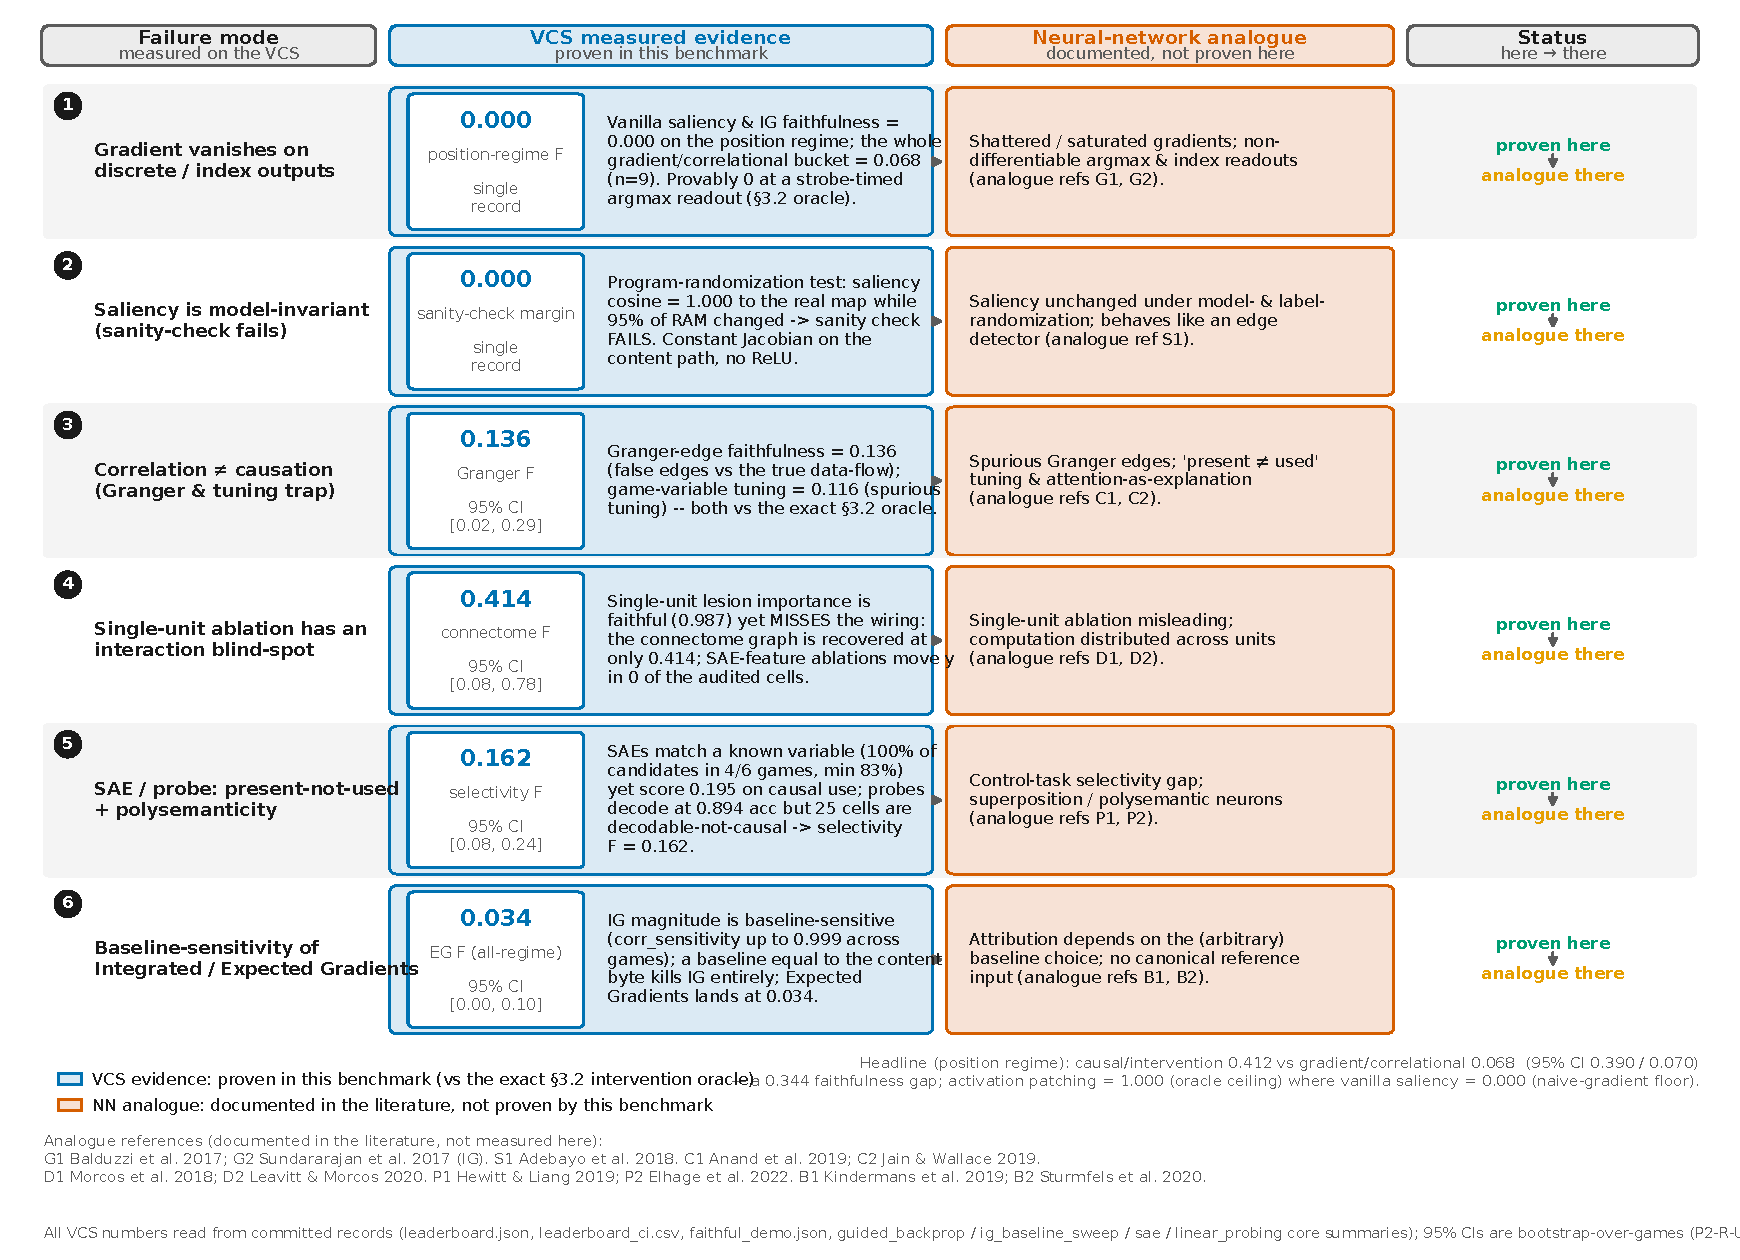
\includegraphics[width=\textwidth]{../figures/fig5_representativeness_map_full.pdf}
\caption{\textbf{Full VCS-to-NN representativeness map.} The full-density version of the
main-text map (Fig.~\ref{fig:representativeness}): each VCS failure mode is placed against its documented
neural-network analogue from the literature. The neural-network column records documented
analogues, not parallels proven by this benchmark; the oracle is the intervention oracle of
\Sectionname3.2, and the underlying per-method values trace to
\texttt{compare/out/leaderboard.json} via Sec.~\ref{supp:provenance}. Note that this full
map is the figure the simplified main-text version condenses.}
\label{supp:fig:repmap}
\end{figure}

\begin{figure}[t]
\centering
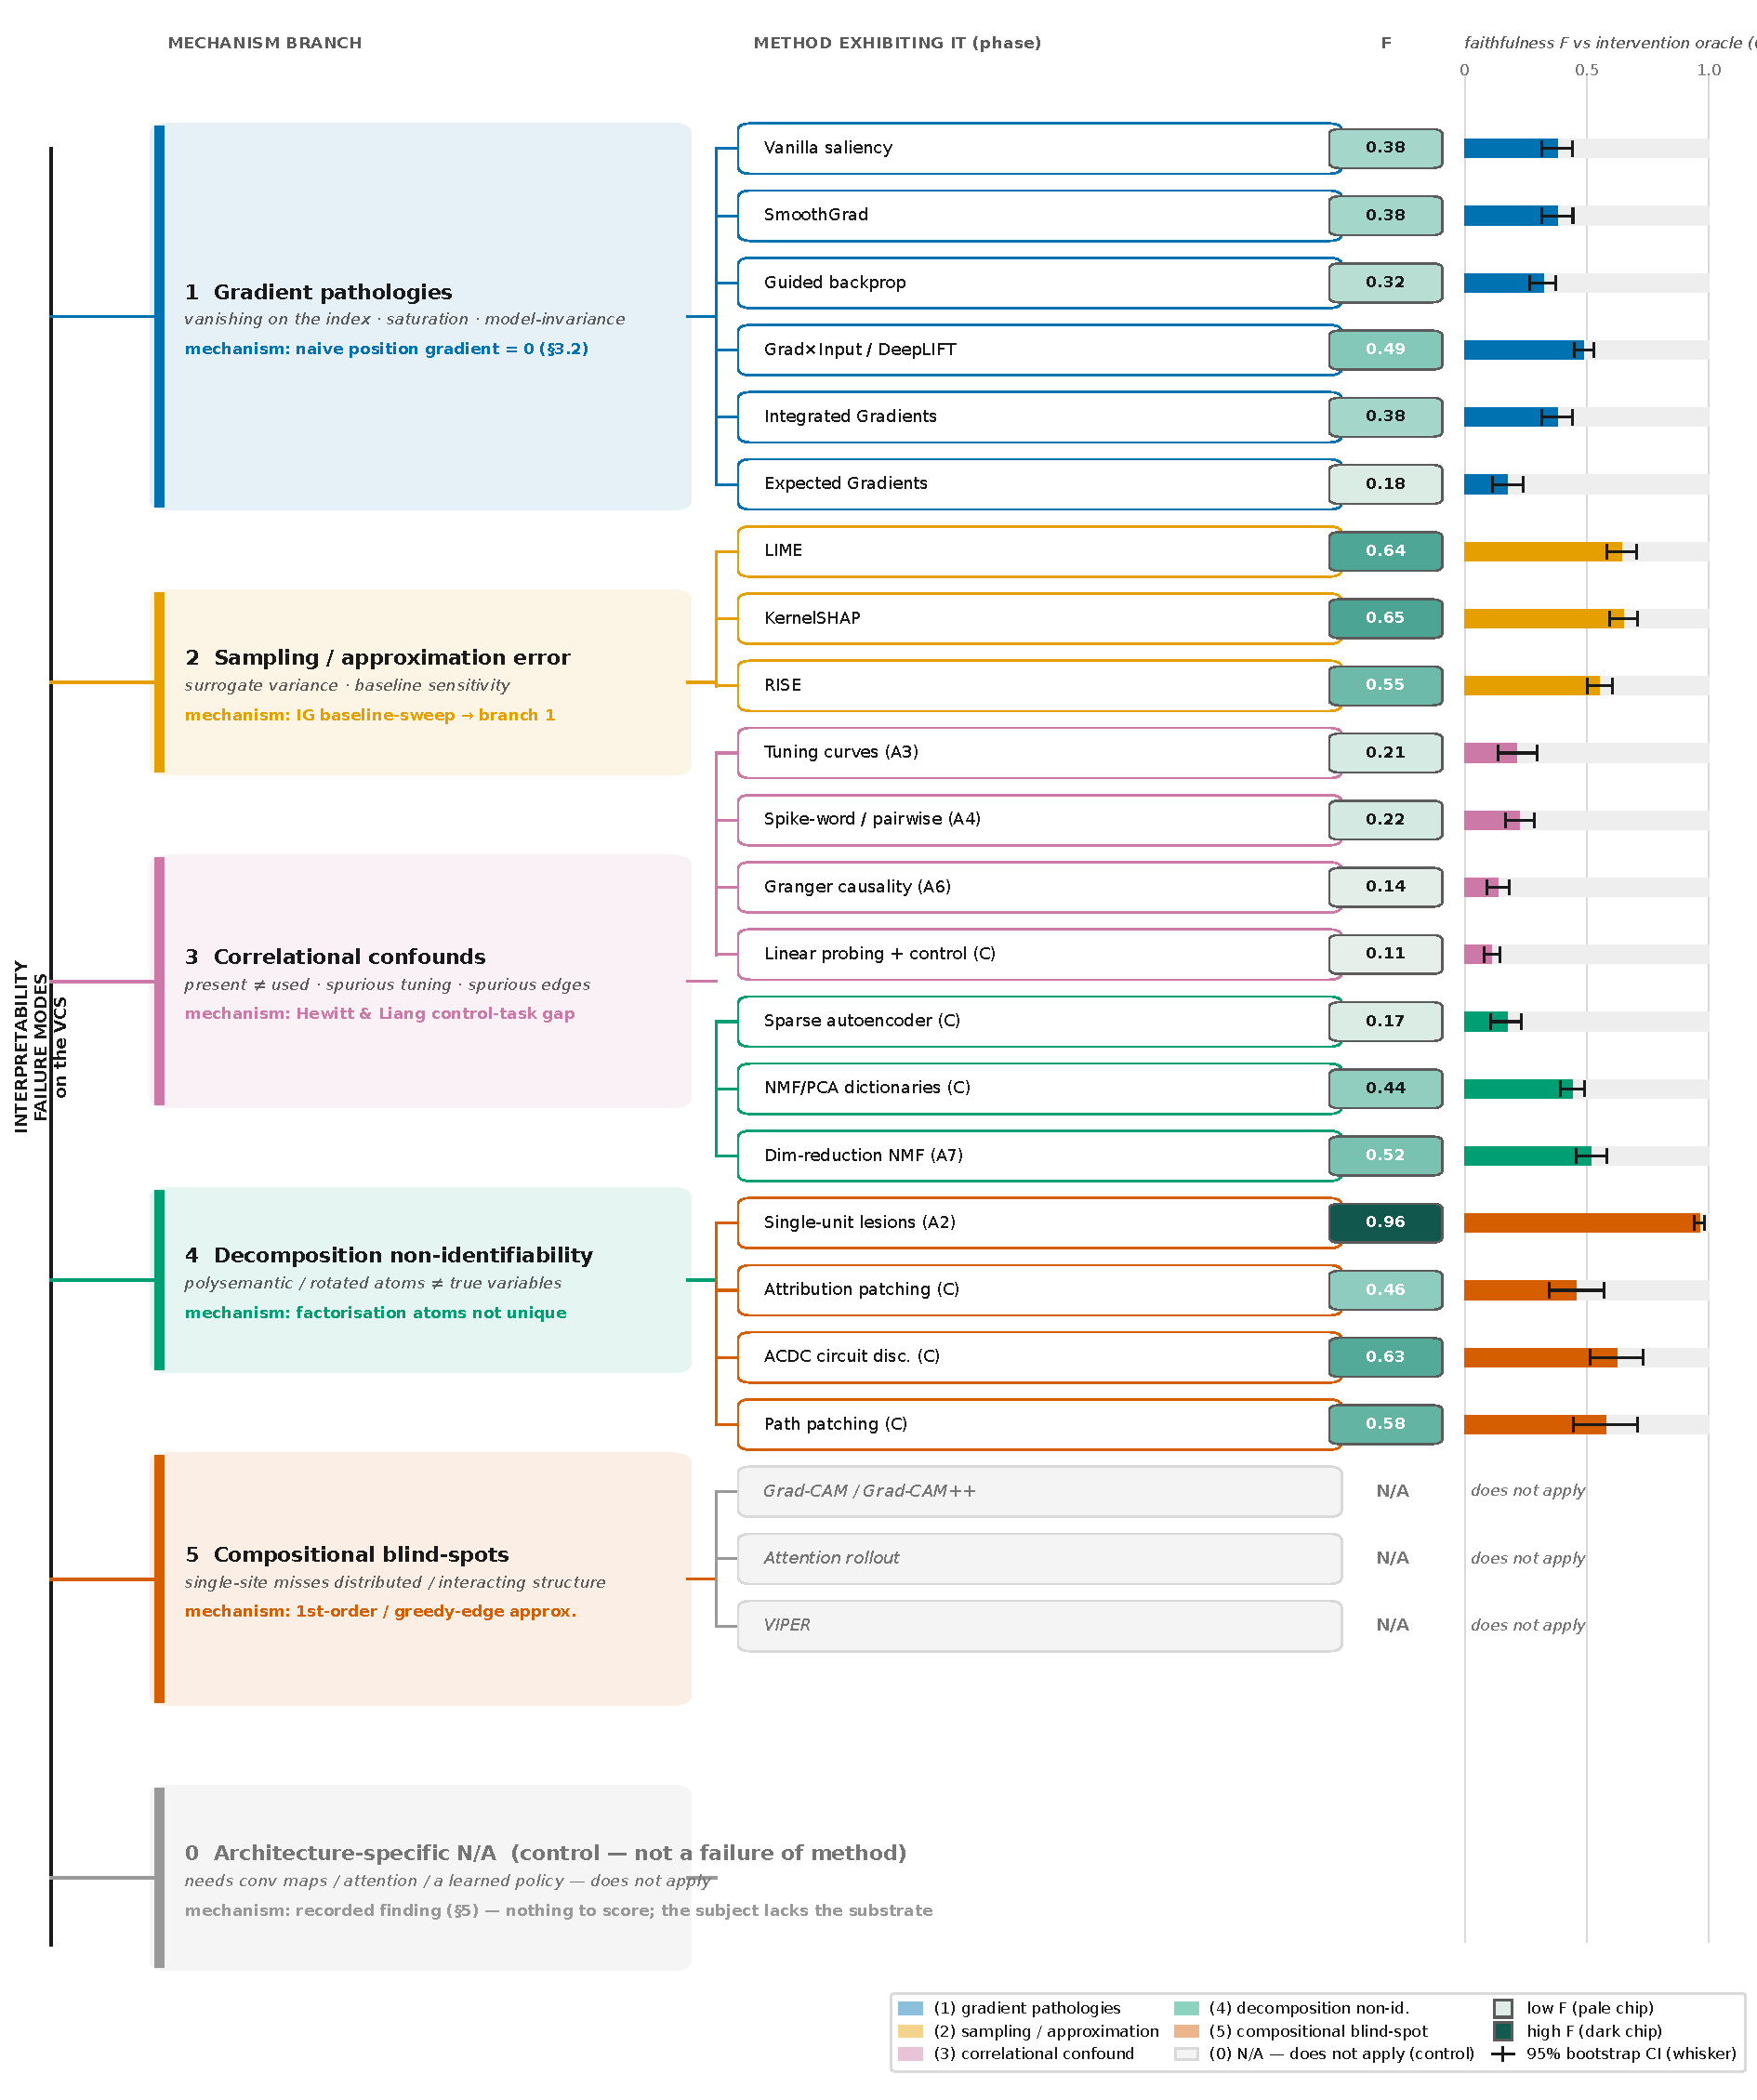
\includegraphics[width=\textwidth]{../figures/fig6_failure_taxonomy_full.pdf}
\caption{\textbf{Full failure taxonomy.} The full-density version of the main-text taxonomy
(Fig.~\ref{fig:taxonomy}): the families of interpretability failure observed on the machine, each annotated
with its faithfulness against the intervention oracle (\Sectionname3.2), reported as $F$ with its
$95\%$ bootstrap confidence interval. The leaf values trace to
\texttt{compare/out/leaderboard.json} and \texttt{leaderboard\_ci.csv} via
Sec.~\ref{supp:provenance}. Note that the gradient and correlational branches collapse on
the discrete position regime, where the naive gradient is provably zero (Prop.~\ref{prop:zero}).}
\label{supp:fig:taxonomy}
\end{figure}

\section{Plausibility-proxy rubric and its sensitivity}\label{supp:plausibility}

The plausibility axis of the leaderboard is a documented, tradition-level proxy, not a
human-subjects measurement. This section records how each value was assigned. It also shows
that the headline contrast does not depend on the particular numbers chosen. The Methods
(\Sectionname\ref{sec:triad}) name two reporting axes. Faithfulness is measured on the machine against the
intervention oracle of \Sectionname\ref{sec:oracle}. The plausibility proxy stands in for how convincing a
tradition's explanations are usually taken to be. We assign the proxy once per method
tradition, before any faithfulness score on our machine is computed, so it cannot be tuned to
the result. Its only job is to expose the danger zone of explanations that look convincing yet
are unfaithful. For that job it must be coarse, fixed in advance, and sourced rather than
precise.

The rubric assigns one proxy per tradition on a fixed five-step scale. It scores two
documented properties of each tradition's typical output and takes their average. The first
property is whether the explanation produces a dense, picture-like artifact that a reader sees
as an account of the computation. Heatmaps and saliency-style maps over the input are read as
convincing by construction. This is the perceptual-immediacy axis. The second property is
whether the field has historically treated the tradition's output as a self-evident
explanation rather than a hypothesis to be tested. This is the adoption-as-explanation axis. A
tradition that scores high on both, such as gradient saliency, receives a high proxy. A
tradition whose output is an austere intervention table or a circuit edge list, rarely
mistaken for a finished story, receives a low one. The scale is deliberately blunt,
$\{0.3,0.5,0.55,0.75,0.8,0.85,0.9\}$. A proxy meant to expose a danger zone gains nothing from
false precision, and a finer scale would invite over-reading. Every value in
Table~\ref{supp:tab:plausrubric} traces to the \jkey{plausibility_proxy} field of the
per-method rows in \texttt{compare/out/leaderboard.json}. The table only groups those rows by
tradition and records the rationale.

\begin{table}[t]
\centering
\caption{\textbf{Plausibility-proxy rubric.} The proxy assigned to each method tradition,
with the documented rationale. Values are the \jkey{plausibility_proxy} field of the
leaderboard rows (\texttt{compare/out/leaderboard.json}). They are tradition-level and fixed
before any faithfulness score is computed, so the proxy cannot be tuned to the measured
faithfulness. A higher value means an explanation that the field tends to find more
convincing, not one that is more faithful. The oracle (\Sectionname\ref{sec:oracle}) is the positive control and
is not a method under test.}
\label{supp:tab:plausrubric}
\begin{tabular}{@{}llp{6.4cm}@{}}
\toprule
Tradition & Proxy & Rationale (documented basis) \\
\midrule
gradient        & $0.90$ & Dense input-space heatmaps read as a visual account of the
                            decision; the most widely adopted XAI outputs, routinely shown
                            as if self-explanatory. \\
probing         & $0.85$ & A trained decoder that ``finds'' a concept reads as evidence the
                            concept is used; high adoption, though decodability is not
                            causal use. \\
correlational   & $0.80$ & Tuning curves and coupling spectra match the neuroscience idiom
                            of a convincing single-unit account. \\
dim.\ reduction & $0.75$ & Low-dimensional factors and dictionary atoms look like a clean
                            summary of the representation. \\
intervention    & $0.55$ & Occlusion and counterfactual outputs are quantitative tables, less
                            immediately picture-like, treated as tests rather than stories. \\
causal          & $0.50$ & Circuit edge lists and patching results are austere artifacts
                            rarely mistaken for a finished narrative. \\
descriptive     & $0.30$ & Whole-state recording is an explicit non-explanation: it withholds
                            nothing and reads as a dump, not an account. \\
\midrule
oracle (control)& $1.00$ & The \Sectionname\ref{sec:oracle} ground truth by construction; positive control, not a
                            method under test. \\
\bottomrule
\end{tabular}
\end{table}

The paper draws a contrast between this proxy and measured faithfulness. On the committed
records the two move in opposite directions. Across the thirty methods under test the Spearman
rank correlation between faithfulness and the proxy is $-0.36$, a negative association.
The traditions the field finds most convincing are, on this machine, among the least faithful.
Eight methods fall in the danger zone, defined here as a proxy of at least $0.70$ together
with a faithfulness below $0.40$. They include the correlational neuroscience methods, Expected
Gradients, guided backprop, linear probing, and the sparse autoencoder. The per-method extreme
makes the point sharply. Vanilla saliency has the highest proxy, $0.9$, yet scores faithfulness
$0.115$ on the position regime. Activation patching has a lower proxy, $0.5$, and scores $1.0$.
Here the less faithful method is the more plausible one. These figures are produced by
\texttt{tools/xai\_study/compare/plausibility\_sensitivity.py} from the leaderboard and
recorded in \texttt{compare/out/plausibility\_sensitivity.csv}.

A proxy fixed by a coarse rubric raises the question of whether the contrast is an artifact of
the particular numbers. The answer is that it is not. We perturb the proxy under four
deterministic schemes and recompute the relationship each time. The analysis uses fixed,
index-keyed offsets rather than random draws, so it re-derives bit-for-bit. The first scheme
adds a fixed per-method jitter of magnitude $\sigma\in\{0.05,0.1,0.2\}$, alternating in sign by
row. The second compresses every proxy toward the common mean by a fraction $\sigma$, which
preserves the rank order of traditions. The third uses the same index-keyed offsets at
$\sigma\in\{0.1,0.2\}$, large enough to swap neighbouring traditions' ranks. The fourth drops
one whole tradition at a time and recomputes on the remainder. Across all fourteen
perturbations the rank correlation between faithfulness and proxy stays negative. It ranges
from $-0.76$ to $-0.08$. The danger zone stays populated, with
between four and ten methods. The per-method anchor sign holds in every scheme where both
anchor methods are present, the more plausible saliency remaining the less faithful. Two runs
bound the range. The strongest is the leave-the-gradient-tradition-out run. It removes the most
plausible and least faithful block at once, and still leaves six danger-zone methods and a rank
correlation of $-0.76$. The weakest is the leave-the-causal-tradition-out run, where the
correlation falls to $-0.08$, close to zero; removing the faithful causal block flattens the
association, so the contrast is carried in part by that block. Table~\ref{supp:tab:plaussens}
reports the full sweep. The contrast keeps its sign under every alternative proxy assignment we
tried: plausibility and faithfulness are not the same axis, and high plausibility is no
guarantee of faithfulness.

\begin{table}[t]
\centering
\caption{\textbf{Proxy-sensitivity sweep.} The faithfulness-versus-proxy relationship under
each perturbation, from \texttt{compare/out/plausibility\_sensitivity.csv}. ``$\rho$'' is the
Spearman rank correlation between faithfulness and proxy over the methods present. ``danger''
is the count of high-proxy ($\geq0.70$), low-faithfulness ($<0.40$) methods. ``anchor'' is
$1$ when the more plausible saliency is the less faithful of the saliency/activation-patching
pair, and blank where a leave-one-out run removes an anchor. The baseline rubric is the first
row. Across every scheme the correlation stays negative and the danger zone stays populated.}
\label{supp:tab:plaussens}
\begin{tabular}{@{}llrrrc@{}}
\toprule
Scheme & Param & $n$ & $\rho$ & Danger & Anchor \\
\midrule
baseline                & ---           & 30 & $-0.36$ &  8 & 1 \\
additive jitter         & $\sigma=0.05$ & 30 & $-0.40$ &  8 & 1 \\
additive jitter         & $\sigma=0.10$ & 30 & $-0.41$ &  8 & 1 \\
additive jitter         & $\sigma=0.20$ & 30 & $-0.42$ & 10 & 1 \\
rank-preserving         & $\sigma=0.10$ & 30 & $-0.36$ &  8 & 1 \\
rank-preserving         & $\sigma=0.20$ & 30 & $-0.36$ &  8 & 1 \\
rank-jittering          & $\sigma=0.10$ & 30 & $-0.41$ &  8 & 1 \\
rank-jittering          & $\sigma=0.20$ & 30 & $-0.42$ & 10 & 1 \\
leave-out causal        & ---           & 24 & $-0.08$ &  8 & \\
leave-out correlational & ---           & 26 & $-0.40$ &  4 & 1 \\
leave-out descriptive   & ---           & 29 & $-0.29$ &  8 & 1 \\
leave-out dim.\ red.    & ---           & 27 & $-0.34$ &  7 & 1 \\
leave-out gradient      & ---           & 20 & $-0.76$ &  6 & \\
leave-out intervention  & ---           & 25 & $-0.34$ &  8 & 1 \\
leave-out probing       & ---           & 29 & $-0.36$ &  7 & 1 \\
\bottomrule
\end{tabular}
\end{table}

; the tables
%% render without overfull boxes and the two SI figures resolve from ../figures/.

\clearpage
\appendix

%% Breakable monospaced JSON key: lets long under_scored keys wrap inside narrow table
%% columns. Used by S5 (number provenance). Defined here so the S-files stay self-contained.
\providecommand{\jkey}[1]{\texttt{\expandafter\jkeyaux#1\relax}}
\makeatletter
\def\jkeyaux#1{\ifx\relax#1\else
  \ifx_#1\discretionary{}{}{}\char`\_\else
    \ifx.#1\discretionary{}{}{}.\else#1\fi\fi
  \expandafter\jkeyaux\fi}
\makeatother

\section*{Supplementary Information}
\setcounter{table}{0}
\setcounter{figure}{0}
\renewcommand{\thetable}{S\arabic{table}}
\renewcommand{\thefigure}{S\arabic{figure}}
\renewcommand{\thesection}{S\arabic{section}}
\setcounter{section}{0}

This Supplementary Information records what the main paper summarizes. We give the
per-method protocols (\Sectionname\ref{supp:protocols}) and the leaderboard schema with its glossary
(\Sectionname\ref{supp:schema}). We give the coverage and applicability of every method across games
and output regimes (\Sectionname\ref{supp:coverage}). We map each headline claim to its evidence
(\Sectionname\ref{supp:claims}). We trace the provenance of every headline number down to the record
file and command that produced it (\Sectionname\ref{supp:provenance}). We state plainly what the
paper does not claim (\Sectionname\ref{supp:notclaimed}). We give the plausibility-proxy rubric and
its sensitivity analysis (\Sectionname\ref{supp:plausibility}). The main text shows simplified forms
of two diagnostic figures; we reproduce both here at full resolution
(Figs.~\ref{supp:fig:repmap} and~\ref{supp:fig:taxonomy}).
The correctness triad $\mathrm{F}\wedge\mathrm{S}\wedge\mathrm{M}$ used throughout is the
one defined in the main Methods (\Sectionname\ref{sec:triad}); we reference it here rather than restating it. The
benchmark scores 30 interpretability methods together with the intervention oracle (\Sectionname\ref{sec:oracle})
as a positive control, for 31 leaderboard rows in total.

\section{Per-method protocols}\label{supp:protocols}

This section records five things for each method under test. It records the exact objects the
method consumes and produces, the reference it is scored against, its sampling or optimization
budget, the metric that turns its output into a faithfulness score, and the committed record
file (version-controlled, in the released repository) that holds the per-game results. All methods share one evaluation contract. We state that
contract once and then specialize it per method. Every method receives the same bit-exact VCS
state on each game of the scored set. We state the contract on the six core games
(\texttt{breakout}, \texttt{ms\_pacman}, \texttt{pong}, \texttt{qbert}, \texttt{seaquest},
\texttt{space\_invaders}), which carry the full tiered ground truth and the exact oracle and
serve as the running example; the aggregate leaderboard scores extend the identical protocol
to the 42-game scored set of \Sectionname\ref{supp:scoredset}. That state is not the boot screen.
It is a shared gameplay state, produced by a single seeded random-action stream (seed~$0$) run
for a $90$-frame prefix and then rolled forward for a $15$-frame analysis horizon. The stream is
deterministic, so every method sees the identical state on each game, and the run is asserted
bit-exact per game. An oracle cause-density gate screens the state before any method runs. The
gate counts how many candidate causes move the output above a floor and rejects states with too
few, so a near-flat oracle column cannot pass. This gate is what turns a degenerate frame into a
usable one; on \texttt{seaquest} it raises the count of live candidate causes from $2$ to $19$.
The candidate-cause set is the machine's own state. This set is the RAM bytes together with the
CPU registers and the TIA and RIOT registers exposed by the substrate. The output every method
attributes over is a shared screen-buffer region read at the end of the analysis horizon, not a
single hand-picked pixel. The reference is the intervention oracle of \Sectionname\ref{sec:oracle},
evaluated by exact re-runs of the emulator under $\mathrm{do}(u)$. A method that
cannot be applied to a given output regime is recorded as not-applicable rather than scored
as zero. An empty result is therefore never read as a wrong one. Faithfulness is the F
axis of the main-text triad (\Sectionname\ref{sec:triad}); we reference that definition and do not restate it.
Records live under \texttt{tools/xai\_study/<phase>/out/}; the aggregate they feed is
\texttt{tools/xai\_study/compare/out/leaderboard.json}.
Table~\ref{supp:leaderboard} consolidates the triad scores for all thirty methods and the
oracle positive control in one place; the per-method protocols follow.

\begin{table*}[t]
\centering
\caption{\textbf{Consolidated leaderboard: all methods, all triad axes.} One row per method
across the three phases, plus the intervention oracle as a positive control. $F$ is
faithfulness (Pearson correlation against the oracle, with the bootstrap-over-games 95\% CI in
brackets), $S$ is sufficiency, $M$ is minimality, all as defined in \Sectionname\ref{sec:triad};
Plaus is the elicited plausibility prior and $n$ is the number of scored games. Attribution
methods that emit only a saliency have no defined $S$ or $M$ and are marked ``---''; A5
(field potentials) and A7 (dimensionality reduction) likewise lack the $S$/$M$ decomposition.
Values are transcribed from \texttt{tools/xai\_study/compare/out/leaderboard.json} (the
committed numbers of record).}
\label{supp:leaderboard}
\footnotesize
\setlength{\tabcolsep}{4pt}
\begin{tabularx}{\textwidth}{@{}Xccccccc@{}}
\toprule
Method & Phase & Tradition & $F$ (95\% CI) & $S$ & $M$ & Plaus & $n$ \\
\midrule
A1 connectomics & A & intervention & 0.207 [0.130, 0.293] & 0.971 & 0.967 & 0.55 & 35 \\
A2 lesions & A & intervention & 0.965 [0.942, 0.983] & 0.591 & 1.000 & 0.55 & 42 \\
A3 tuning curves & A & correlational & 0.213 [0.136, 0.295] & 0.200 & 0.928 & 0.80 & 42 \\
A4 spike-word / pairwise & A & correlational & 0.225 [0.166, 0.283] & 0.133 & 0.363 & 0.80 & 34 \\
A5 field potentials & A & correlational & 0.376 [0.323, 0.428] & --- & --- & 0.80 & 40 \\
A6 Granger & A & correlational & 0.136 [0.091, 0.184] & 0.884 & 0.647 & 0.80 & 35 \\
A7 dim.\ reduction & A & dim.\ red. & 0.519 [0.457, 0.581] & --- & --- & 0.75 & 42 \\
A8 whole-state & A & descriptive & 1.000 [1.000, 1.000] & 1.000 & 0.075 & 0.30 & 42 \\
\midrule
Vanilla saliency & B & gradient & 0.380 [0.316, 0.445] & --- & --- & 0.90 & 42 \\
smoothgrad & B & gradient & 0.380 [0.317, 0.445] & --- & --- & 0.90 & 42 \\
Guided backprop & B & gradient & 0.322 [0.267, 0.375] & --- & --- & 0.90 & 42 \\
Grad$\times$Input / DeepLIFT & B & gradient & 0.486 [0.448, 0.526] & --- & --- & 0.90 & 42 \\
Integrated Gradients & B & gradient & 0.379 [0.314, 0.444] & --- & --- & 0.90 & 42 \\
Expected Gradients & B & gradient & 0.175 [0.110, 0.240] & --- & --- & 0.90 & 42 \\
kernelshap & B & gradient & 0.652 [0.596, 0.709] & --- & --- & 0.90 & 42 \\
lime & B & gradient & 0.644 [0.582, 0.705] & --- & --- & 0.90 & 42 \\
rise & B & gradient & 0.552 [0.500, 0.600] & --- & --- & 0.90 & 42 \\
occlusion & B & intervention & 0.687 [0.624, 0.746] & --- & --- & 0.55 & 42 \\
Extremal perturbation & B & intervention & 0.461 [0.410, 0.513] & --- & --- & 0.55 & 42 \\
On-distribution counterfactual & B & intervention & 0.433 [0.343, 0.522] & --- & --- & 0.55 & 42 \\
\midrule
Activation patching & C & causal & 1.000 [1.000, 1.000] & --- & --- & 0.50 & 42 \\
Causal scrubbing & C & causal & 0.979 [0.940, 1.000] & 0.979 & 0.814 & 0.50 & 42 \\
Interchange interventions (DAS) & C & causal & 1.000 [1.000, 1.000] & --- & --- & 0.50 & 42 \\
Logit / tuned lens & C & causal & 0.820 [0.768, 0.871] & --- & 0.224 & 0.50 & 42 \\
Path patching & C & causal & 0.580 [0.452, 0.710] & --- & --- & 0.50 & 42 \\
ACDC & C & causal & 0.625 [0.514, 0.730] & 0.299 & 1.000 & 0.50 & 35 \\
Attribution patching & C & gradient & 0.456 [0.345, 0.573] & --- & --- & 0.90 & 42 \\
Linear probing (+ control) & C & probing & 0.240 [0.153, 0.346] & --- & 0.932 & 0.85 & 42 \\
NMF / PCA dictionaries & C & dim.\ red. & 0.102 [0.049, 0.160] & 0.751 & 0.966 & 0.75 & 42 \\
Sparse autoencoder & C & dim.\ red. & 0.153 [0.096, 0.218] & 0.183 & 0.934 & 0.75 & 40 \\
\midrule
Intervention oracle & --- & oracle & 1.000 [1.000, 1.000] & 1.000 & 1.000 & 1.00 & 1 \\
\bottomrule
\end{tabularx}
\end{table*}

The neuroscience analyses (Phase~A) treat the running machine as a brain. It asks how far
each classical analysis recovers the known mechanism on the shared gameplay state. Each
method's baseline is the exact data-flow graph or causal role that the substrate makes
available. Its budget is the scored set (\Sectionname\ref{supp:scoredset}) unless noted,
with the six-game core as the running example, and its scoring metric is named in
Table~\ref{supp:tab:phaseA}. One core cell is honestly degenerate. On \texttt{ms\_pacman} the
pairwise analysis (A4) finds no coupled candidate pair to score at that frame, so its
\texttt{ms\_pacman} value is uninformative rather than a failure; the other five games carry
it.

\begin{table}[t]
\centering
\caption{\textbf{Phase~A protocols (neuroscience analyses).} One row per method. The columns
give the input it reads, the reference it is scored against, the sampling or intervention
budget, the scoring metric, and the committed record. All eight run on the scored set
(\Sectionname\ref{supp:scoredset}), with the six core games as the running example;
faithfulness is the F axis of \Sectionname\ref{sec:triad}. The whole-state recording (A8) is included as a
descriptive upper bound on coverage. Its faithfulness $F$ is trivial, so we read it for its
minimality $M$.}
\label{supp:tab:phaseA}
\scriptsize
\setlength{\tabcolsep}{4pt}
\begin{tabular}{@{}p{1.7cm}p{2.6cm}p{1.9cm}p{2.6cm}p{1.0cm}@{}}
\toprule
Method & Input / candidate causes & Reference & Scoring metric & Record \\
\midrule
A1 connectomics & RAM/register activity over trajectory & data-flow graph & data-flow graph $F_1$ vs.\ oracle & A1 \\
A2 lesions & single-cell knockouts via $\mathrm{do}(u)$ & true causal role & lesion-importance $\rho$ vs.\ role & A2 \\
A3 tuning curves & per-cell response vs.\ variable & variable coupling & $1-$ spurious-tuning rate & A3 \\
A4 spike-word / pairwise & pairwise cell correlations & true coupling & corr.\ $\rho$ vs.\ coupling & A4 \\
A5 field potentials & pooled-activity spectra & true causal share & $1-$ clock-explained var. & A5 \\
A6 Granger & directed lag structure & true data-flow & $1-$ false-edge rate & A6 \\
A7 dim.\ reduction & NMF/PCA over activity & known variables & NMF matched-component frac. & A7 \\
A8 whole-state & full state record & oracle decomp. & minimality $M$ vs.\ oracle & A8 \\
\bottomrule
\end{tabular}

\smallskip
\noindent\scriptsize Records: \texttt{tools/xai\_study/phaseA\_kording/out/A\{1..8\}\_*}; all
eight run on the 42-game scored set (\Sectionname\ref{supp:scoredset}), with the six core
games as the running example (\jkey{n_games} per method in \jkey{leaderboard.json}).
\end{table}

The attribution methods (Phase~B) run the everyday XAI toolbox over the same gameplay state.
These methods produce a real-valued saliency or attribution over the candidate-cause set.
We score that output by Pearson correlation against the oracle attribution. The gradient family
runs with the bilinear sub-pixel sampler turned on, so it is scored on a real position gradient
and not on the naive one. The naive gradient of the discrete position output is provably zero
(Prop.~\ref{prop:zero}); the sampler restores a finite gradient, but the restored gradient is
low and mixed in faithfulness rather than a fix. Expected Gradients draws its reference pool
from the states of the same seeded gameplay trajectory, not from a synthetic baseline. Two cells
are honestly degenerate and recorded as such. The on-distribution counterfactual returns a zero
delta on \texttt{space\_invaders}, \texttt{ms\_pacman}, and \texttt{qbert}, where its perturbation
does not move the shared output at that frame; those cells are marked not-valid rather than
scored. Expected Gradients scores low on the content regime of every game except \texttt{pong},
because the causal byte it should land on is static there. The budgets that matter are the
Monte-Carlo or perturbation counts of the sampling estimators, recorded per method in
Table~\ref{supp:tab:phaseB}. The seed-dispersion of the stochastic members is carried in
\texttt{leaderboard\_ci.csv} (\texttt{seed\_sd}, \texttt{seed\_sd\_source}) and reproduced
in \Sectionname\ref{supp:provenance}.

\begin{table}[t]
\centering
\caption{\textbf{Phase~B protocols (attribution methods).} Each method emits a saliency over
the candidate-cause set. We score it by Pearson correlation against the oracle attribution
(\Sectionname\ref{sec:oracle}). The reference is shared and the budget is the scored set of
\Sectionname\ref{supp:scoredset} (six core games as the running example). The budget column records the
sampling or perturbation count that drives each estimator. The seed column flags which
methods carry an independent-seed dispersion in \texttt{leaderboard\_ci.csv}.}
\label{supp:tab:phaseB}
\scriptsize
\setlength{\tabcolsep}{4pt}
\begin{tabular}{@{}p{2.9cm}p{1.75cm}p{4.3cm}p{1.15cm}@{}}
\toprule
Method & Tradition & Budget / hyperparameters & Seed sd \\
\midrule
Vanilla saliency & gradient & single backward pass & --- \\
smoothgrad & gradient & noise-averaged gradient; $\sigma$-robustness committed & 0.0 \\
Guided backprop & gradient & single guided pass & --- \\
Grad$\times$Input / DeepLIFT & gradient & DeepLIFT reference-difference & --- \\
Integrated Gradients & gradient & path integral, baseline = zero state & --- \\
Expected Gradients & gradient & expectation over baselines (refits) & yes \\
kernelshap & gradient & Monte-Carlo coalition sampling ($\propto 1/\sqrt{N}$) & 0.017 \\
lime & gradient & local linear fit, perturbation refits & 0.029 \\
rise & gradient & random-mask Monte-Carlo ($\propto 1/\sqrt{N}$) & 0.051 \\
occlusion & intervention & exhaustive single-cell masking & --- \\
Extremal perturbation & intervention & optimized mask, area-constrained & --- \\
On-distribution counterfactual & intervention & on-manifold $\mathrm{do}(u)$ resampling & --- \\
\bottomrule
\end{tabular}

\smallskip
\noindent\scriptsize Records: \texttt{tools/xai\_study/phaseB\_attribution/out/}; all twelve run
on the 42-game scored set (\Sectionname\ref{supp:scoredset}), six core games as the running
example, and are scored by Pearson correlation against the oracle (\Sectionname\ref{sec:oracle}). Seed
sd is the independent-seed dispersion from \texttt{leaderboard\_ci.csv}.
\end{table}

The mechanistic methods (Phase~C) are built to recover circuits. Each is scored
against the true data-flow or the exact recovered-minus-exact deviation. The causal members
of this phase are the ones that reach the oracle ceiling. We list their exact scoring metric
so that the ceiling is not read as a tautology. Each member is scored against the substrate's
known routine, and not against another method. Two members (NMF/PCA dictionaries and the
sparse autoencoder) are dimensionality-reduction methods carried here for comparison. The
sparse autoencoder has two aggregations that differ, which we reconcile in
\Sectionname\ref{supp:provenance}.

\begin{table}[t]
\centering
\caption{\textbf{Phase~C protocols (mechanistic methods).} Each method is scored against the
substrate's known circuit or the exact recovered-minus-exact deviation (\Sectionname\ref{sec:oracle}), and not
against another method. This is what keeps the oracle ceiling non-circular. The probing and
dictionary-learning members are included for comparison with the causal members.}
\label{supp:tab:phaseC}
\scriptsize
\setlength{\tabcolsep}{4pt}
\begin{tabular}{@{}p{3.4cm}p{1.4cm}p{5.2cm}@{}}
\toprule
Method & Tradition & Scoring metric \\
\midrule
Activation patching & causal & $\max|\text{recovered}-\text{exact}|$ vs.\ oracle \\
Causal scrubbing & causal & scrubbing-preserved performance \\
Interchange interventions (DAS) & causal & aligned interchange accuracy \\
Logit / tuned lens & causal & logit-lens fidelity to true intermediate \\
Path patching & causal & path-circuit $F_1$ vs.\ true routine \\
ACDC & causal & discovered-circuit best $F_1$ vs.\ data-flow \\
Attribution patching & gradient & corr.\ of approximation vs.\ exact patch \\
Linear probing (+ control) & probing & selectivity vs.\ control task \\
NMF / PCA dictionaries & dim.\ red. & matched-component fraction vs.\ vars \\
Sparse autoencoder & dim.\ red. & feature-variable matched fraction \\
\bottomrule
\end{tabular}

\smallskip
\noindent\scriptsize Records: \texttt{tools/xai\_study/phaseC\_mechanistic/out/}; all ten run
on the 42-game scored set (\Sectionname\ref{supp:scoredset}), with the six core games as the
running example.
\end{table}

The intervention oracle is the positive control, not a method under test. It is the exact
$\mathrm{do}(u)$ ground truth of \Sectionname\ref{sec:oracle}, evaluated by re-running the bit-exact machine. It
attains $F=S=M=1.0$ by construction. Its record triple is the intervention oracle, the
content-path gradient oracle, and their cross-check
(\texttt{tools/xai\_study/ground\_truth/out/}). It anchors the ceiling against which every
other row is read, which is why it occupies the thirty-first leaderboard row.

\section{Benchmark schema and glossary}\label{supp:schema}

The leaderboard is built from a flat record schema. Stating it removes the ambiguity
about what a single number on the benchmark counts. Each method is run per game and writes a
per-game record under its phase's \texttt{out/} tree. The leaderboard aggregates those
records into one row per method by averaging over games. The schema columns of a leaderboard
row are given in Table~\ref{supp:tab:schema}. The aggregation rule is a mean over the
$n_{\text{games}}$ games. When a method emits several output records on one game, those records
are first reduced within that game. The faithfulness, sufficiency, and minimality columns
report the F, S, and M axes defined in \Sectionname\ref{sec:triad}. We do not re-derive those definitions here.

\begin{table}[t]
\centering
\caption{\textbf{Leaderboard row schema.} The columns of one row in
\texttt{compare/out/leaderboard.json} (\texttt{rows[\,]}) and its uncertainty companion
\texttt{leaderboard\_ci.csv}. The metric column names the per-method scoring function from
\Sectionname\ref{supp:protocols}; F, S, and M are the triad axes of \Sectionname\ref{sec:triad}. Aggregation is a mean
over $n_{\text{games}}$, with bootstrap confidence intervals over games (and, where present,
over records).}
\label{supp:tab:schema}
\footnotesize
\begin{tabular}{@{}p{3.0cm}p{8.4cm}@{}}
\toprule
Column & Meaning \\
\midrule
\texttt{phase} & phaseA\_kording, phaseB\_attribution, phaseC\_mechanistic, or ground\_truth \\
\texttt{method} & method identifier (the row key) \\
\texttt{tradition} & intervention, causal, gradient, correlational, \jkey{dim_reduction}, probing, descriptive, oracle \\
\jkey{n_games} & number of games the method was scored on (up to 42 for the scored set of \Sectionname\ref{supp:scoredset}; 1 for the oracle) \\
\jkey{n_records} & number of per-game output records aggregated into the row \\
\texttt{faithfulness} (F) & faithfulness vs.\ the intervention oracle (\Sectionname\ref{sec:oracle}), $[0,1]$, higher better \\
\jkey{faithfulness_ci95} & $95\%$ bootstrap CI half-width over games \\
\jkey{faithfulness_position_regime} & F restricted to the discrete sprite-position/index regime \\
\jkey{faithfulness_content_regime} & F restricted to the continuous content regime \\
\texttt{triad\_S} / \texttt{triad\_M} & sufficiency / minimality axes (\Sectionname\ref{sec:triad}), where applicable \\
\jkey{plausibility_proxy} & documented method-tradition proxy, $[0,1]$ --- not a human-subjects measurement \\
\jkey{is_positive_control} & 1 for the oracle row, 0 otherwise \\
\jkey{metric_names} & the per-method scoring function (\Sectionname\ref{supp:protocols}) \\
\texttt{commits} & the commit(s) at which the per-game records were produced \\
\bottomrule
\end{tabular}
\end{table}

We fix the vocabulary that the schema implies, because the review asked for a single
unambiguous method count. A \emph{method} is one interpretability technique, e.g.\
\texttt{vanilla\_saliency}. A \emph{method row} is its single aggregated line on the
leaderboard. A \emph{per-game record} is one method scored on one game, written under a phase
\texttt{out/} tree. An \emph{output record} is a per-game record for one output regime; a
method may emit several of these on one game. A \emph{family mean} is the average over the
members of a tradition family, e.g.\ causal/intervention. The \emph{oracle positive control}
is the exact $\mathrm{do}(u)$ ground truth of \Sectionname\ref{sec:oracle}, scored as a method to anchor the
ceiling. A \emph{not-applicable method} is one that does not apply to a given output regime;
it is recorded as N/A rather than as a zero. With this vocabulary the count is unambiguous.
The benchmark scores 30 interpretability methods together with the intervention
oracle as a positive control, for 31 leaderboard rows in total
(\texttt{leaderboard.json.n\_methods}~$=31$), aggregating 1773 per-game records over the
42-game scored set (\texttt{n\_per\_game\_records\_aggregated}~$=1773$): 8 methods in
Phase~A, 12 in Phase~B, 10 in Phase~C, and the one oracle row. This count is the canonical one
used in the abstract, the figures, and throughout this Supplement.

\section{Coverage and applicability}\label{supp:coverage}

The benchmark scores methods on a six-game core drawn from a larger bit-exact substrate. The
coverage table makes the scope of that choice explicit. Paper~1 validates the
differentiable VCS ports bit-for-bit against the \texttt{xitari} reference on all 64 Arcade
Learning Environment games, within a 30-frame RAM and 60-frame screen window. The
interpretability study reported here runs on the six games listed in
Table~\ref{supp:tab:coverage}. Every method is scored on a shared gameplay state, produced by
one seeded random-action stream (seed~$0$, $90$-frame prefix, $15$-frame analysis horizon), not
on the boot screen. This keeps the analysis inside the Paper~1 bit-exact window while giving the
oracle a rich, non-degenerate cause set to score against. We pick these six games because all
three tiers of ground truth (\Sectionname\ref{sec:tiers}) are available for them and the oracle is
exact. The remaining 58 games are
bit-exact substrate but are not scored here. Some fall outside the validated horizon for the
analyses we run. For others, the tiered labels they would need are not yet produced. They are
candidates for the larger sweep, and are not excluded for any methodological reason. The
horizon column records the validated window. The tier column records which of the three
ground-truth tiers (T1 exact intervention, T2 data-flow, T3 externally-supplied semantic
labels) is available.

\begin{table}[t]
\centering
\caption{\textbf{Core-game coverage.} The six core games carry exact tiered ground truth and
the full method battery. Faithfulness is scored within the Paper~1 bit-exact window. The
last two columns give the methods run and the per-game output records contributed. The wider
64-game substrate is bit-exact (Paper~1) but is reserved for the larger sweep. T3 labels are
external (\Sectionname\ref{sec:tiers}); we record this so the benchmark does not appear to certify them.}
\label{supp:tab:coverage}
\footnotesize
\setlength{\tabcolsep}{4pt}
\begin{tabular}{@{}p{2.4cm}p{1.9cm}p{1.5cm}p{1.7cm}p{1.5cm}p{1.4cm}@{}}
\toprule
Game & Paper-1 status & Horizon & Tiers & Methods run & Records \\
\midrule
breakout & bit-exact & 30/60 fr & T1,T2,T3 & 30 + oracle & per-game \\
ms\_pacman & bit-exact & 30/60 fr & T1,T2,T3 & 30 + oracle & per-game \\
pong & bit-exact & 30/60 fr & T1,T2,T3 & 30 + oracle & per-game \\
qbert & bit-exact & 30/60 fr & T1,T2,T3 & 30 + oracle & per-game \\
seaquest & bit-exact & 30/60 fr & T1,T2,T3 & 30 + oracle & per-game \\
space\_invaders & bit-exact & 30/60 fr & T1,T2,T3 & 30 + oracle & per-game \\
\midrule
58 further games & bit-exact (P1) & 30/60 fr & T1,T2 partial & reserved & --- \\
\bottomrule
\end{tabular}
\end{table}

A gameplay state can still be degenerate for a particular method, and the benchmark records
this rather than scoring it as a failure. The oracle cause-density gate is the first guard. It
counts how many candidate causes move the shared output above a floor, and rejects a state that
does not clear a minimum count, so a near-flat oracle column never reaches a method. On
\texttt{seaquest} the gate raises the count of live candidate causes at the analysis frame from
$2$ to $19$, which is what makes the game usable. Three residual degenerate cells survive the
gate and are marked, not scored as zero. On \texttt{ms\_pacman} the pairwise neuroscience
analysis (A4) finds no coupled candidate pair at that frame, so its cell is uninformative. The
on-distribution counterfactual returns a zero delta on \texttt{space\_invaders},
\texttt{ms\_pacman}, and \texttt{qbert}, where its perturbation does not move the shared output;
those cells are recorded as not-valid. Expected Gradients scores low on the content regime of
every game but \texttt{pong}, because the causal byte it should attribute to is static there.
None of these cells is read as a wrong answer.

Whether a method applies at all depends on what the method needs from its target. The
applicability matrix records that for every method family. The Phase~A neuroscience analyses
read the raw machine state and need neither a learned policy nor gradients. The Phase~B
attribution methods split into two groups. The gradient members need a differentiable forward
pass. The intervention members need only the ability to set state. The Phase~C mechanistic
methods need access to internal activations. The causal members among them also need the
ability to intervene. Table~\ref{supp:tab:applic} records, per family, whether the method
operates on the raw VCS, whether it requires a learned policy, gradients, internal layers or
attention, or external labels, whether it uses oracle-like interventions, and whether it
receives a supplied hypothesis. The table shows the same pattern the results confirm. The
families that score high on faithfulness are the ones that can intervene. The families that
collapse on the position regime are the gradient and correlational ones.

\begin{table}[t]
\centering
\caption{\textbf{Per-family applicability.} What each method family requires of its target.
``Intervenes'' marks oracle-like $\mathrm{do}(u)$ access; ``hypothesis'' marks methods that
receive a supplied circuit hypothesis to test. The raw-VCS column distinguishes analyses that
read machine state directly from those that need a differentiable or layered model. A blank
means the requirement does not apply.}
\label{supp:tab:applic}
\footnotesize
\begin{tabular}{@{}p{3.0cm}cccccc@{}}
\toprule
Family & raw VCS & policy & gradients & layers/attn & intervenes & hypothesis \\
\midrule
A neuroscience & yes & no & no & no & A2 only & no \\
B gradient & yes & no & yes & no & no & no \\
B intervention & yes & no & no & no & yes & no \\
C causal & yes & no & no & yes & yes & yes \\
C gradient (attr.\ patch) & yes & no & yes & yes & approx. & yes \\
C probing & yes & no & no & yes & no & no \\
C / A dim.\ reduction & yes & no & no & yes & no & no \\
oracle (control) & yes & no & no & yes & exact & --- \\
\bottomrule
\end{tabular}
\end{table}

\section{Claims and evidence}\label{supp:claims}

Every headline claim in the paper rests on a specific artifact. The table in this section
makes that dependency checkable. For each claim we list the figure or table that supports it,
the games and methods it uses, the metric, the artifact it traces to, and the limitation that
bounds it. Faithfulness, sufficiency, and minimality are the three axes of \Sectionname\ref{sec:triad}.
The numbers themselves are sourced in \Sectionname\ref{supp:provenance}. The table below names which
evidence supports which claim; it does not repeat the values. One split matters for how the
table is read. The all-regime faithfulness gap between causal/intervention and
gradient/correlational methods is $0.297$ with a $95\%$ interval of $[0.232,0.375]$ that
excludes zero, and it is the primary evidence for the headline. The position-only gap is
$0.238$ with an interval of $[-0.049,0.315]$ that crosses zero at six games. We report the
position gap as directional support, not as a significant result.

\begin{table}[t]
\centering
\caption{\textbf{Claims and their evidence.} Each headline claim maps to the figure or table
that supports it, the games and methods involved, the metric, the committed artifact, and the
limitation that bounds the claim. The artifact column points to the record that
\Sectionname\ref{supp:provenance} traces to a value. The limitation column states the scope, so the
claim is not read wider than the evidence.}
\label{supp:tab:claims}
\scriptsize
\setlength{\tabcolsep}{4pt}
\begin{tabular}{@{}p{3.0cm}p{1.9cm}p{1.8cm}p{1.9cm}p{2.4cm}@{}}
\toprule
Claim & Evidence & Methods / games & Metric & Limitation \\
\midrule
Causal/intervention methods beat gradient/correlational on faithfulness across all regimes & Fig.~\ref{fig:faithfulness}; leaderboard & 25 methods, 6 games & F mean (gap $0.297$) & robust: gap $0.297$ $[0.232,0.375]$ excludes zero; this all-regime gap is the primary evidence \\
The gap holds with the same sign on the discrete position regime & Fig.~\ref{fig:faithfulness}; \jkey{faithful_demo} & 13 rows, 6 games & F position (gap $0.238$) & directional only: gap $0.238$ $[-0.049,0.315]$ crosses zero at 6 games, so it is not significant \\
A faithful causal method reaches the oracle ceiling where the default tool stays low & \jkey{faithful_demo}; Fig.~\ref{fig:faithfulness} & act.\ patching vs.\ vanilla saliency, 6 games & F $1.0$ vs.\ $0.165$ (position regime; all-regimes saliency F $0.419$, plotted in Fig.~\ref{fig:faithfulness}) & one decisive pair \\
The naive gradient of a discrete position output is provably zero & Prop.~\ref{prop:zero} (\Sectionname\ref{sec:oracle}); \jkey{oracle_grad} & all gradient methods & grad@position $=0$; sampler restores $166$ & position path only; restored gradient is low/mixed \\
High plausibility coexists with low faithfulness (the danger zone) & Fig.~\ref{fig:faithfulness}; \jkey{faithful_demo} & vanilla saliency & proxy $0.9$, F $0.165$ (position regime; all-regimes F $0.419$, plotted in Fig.~\ref{fig:faithfulness}) & proxy, not measured plausibility \\
Faithful attribution recovers the wiring but not the computation's semantics & Fig.~\ref{fig:taxonomy} (\Sectionname\ref{supp:coverage}); discussion & Phase~B vs.\ C & F vs.\ S, M & necessary-condition stress test \\
The failure modes have documented NN analogues & Fig.~\ref{fig:representativeness} & taxonomy & --- & analogues, not proof \\
\bottomrule
\end{tabular}
\end{table}

\section{Number provenance}\label{supp:provenance}

Every headline number traces to a committed record, the script that produced it, and the
command that re-derives it. This section is the in-paper copy of that traceability table. It
mirrors \Sectionname6.5 of the reproducibility document
(\texttt{xai\_2\_interpretability/REPRODUCIBILITY.md}). The values are the measured, committed
ones at the current revision. The position-regime gap and its $95\%$ interval are read from
\texttt{tools/xai\_study/compare/out/position\_bootstrap.json}; the other aggregates from
\texttt{leaderboard.json}, rather than recomputed here. Each
record also carries \texttt{seed}, \texttt{where}, \texttt{commit}, and \texttt{timestamp}, so
the provenance of every value is self-documenting. The aggregate scores below are taken over
the 42-game scored battery of \Sectionname\ref{supp:scoredbattery}, not the six-game core;
each per-method row is a mean over the games on which that method applies (\jkey{n_games}
per method, e.g.\ 42 for most methods, 35 for ACDC and A1). The position-regime gap is now
significant on this battery.

\begin{table}[t]
\centering
\caption{\textbf{Headline-number provenance.} Each number $\rightarrow$ its committed record
and JSON key $\rightarrow$ the generating or aggregating script $\rightarrow$ the command
that reproduces it. Values are the measured, committed numbers at this revision (consistent
with REPRODUCIBILITY \Sectionname6.5); the position-regime gap CI is read from
\jkey{position_bootstrap.json}, all other aggregates from \jkey{leaderboard.json}. Paths are
relative to \texttt{tools/xai\_study/}.}
\label{supp:tab:provenance}
\scriptsize
\setlength{\tabcolsep}{3pt}
\renewcommand{\arraystretch}{1.15}
\begin{tabular}{@{}p{2.5cm}p{1.6cm}p{3.4cm}p{1.9cm}@{}}
\toprule
Number & Value & Record (JSON key) & Command \\
\midrule
Faithfulness gap, all regimes (causal $-$ gradient) & $0.3374$\newline {\scriptsize$[0.3103,0.3643]$, excl.\ $0$} & \jkey{position_bootstrap.json}: \jkey{all\_regime.family\_mean\_gap}, \jkey{ci95} & \jkey{position_bootstrap.py} \\
Causal/interv.\ mean F, all regimes & $0.7215$\newline {\scriptsize$n{=}11$} & \jkey{leaderboard.json}: \jkey{family_causal_intervention} \jkey{mean} & \jkey{leaderboard.py} \\
Gradient/corr.\ mean F, all regimes & $0.384$\newline {\scriptsize$n{=}14$} & \jkey{leaderboard.json}: \jkey{family_gradient_correlational} \jkey{mean} & \jkey{leaderboard.py} \\
Faithfulness gap, position regime (bootstrap over games) & $0.3268$\newline {\scriptsize$[0.1325,0.3702]$, excl.\ $0$} & \jkey{position_bootstrap.json}: \jkey{family_mean_gap}, \jkey{ci95} & \jkey{position_bootstrap.py} \\
Causal/interv.\ mean F, position regime & $0.561$\newline {\scriptsize$\pm0.3212$, $n{=}4$} & \jkey{leaderboard.json}: \jkey{family_..._intervention_position} \jkey{mean} & \jkey{leaderboard.py} \\
Gradient/corr.\ mean F, position regime & $0.2343$\newline {\scriptsize$\pm0.156$, $n{=}9$} & \jkey{leaderboard.json}: \jkey{family_..._correlational_position} \jkey{mean} & \jkey{leaderboard.py} \\
Decisive pair, position regime (act.\ patch vs.\ vanilla sal.) & $1.000$\newline vs.\ $0.115$ & \texttt{faithful\_demo}: \jkey{pair_contrast} & \jkey{faithful_demo.py} \\
Plausibility proxy, decisive pair & $0.5$ vs.\ $0.9$ & \texttt{faithful\_demo}: \jkey{...plausibility_proxy} & \jkey{faithful_demo.py} \\
ACDC sufficiency $S$ & $0.299$ & \jkey{leaderboard.json}: ACDC \jkey{triad_S} & \jkey{leaderboard.py} \\
Whole-state minimality $M$ & $0.0755$ & \jkey{leaderboard.json}: A8 \jkey{triad_M} & \jkey{leaderboard.py} \\
Methods scored (rows) & $31$ & \texttt{leaderboard}: \jkey{n_methods} & \jkey{leaderboard.py} \\
Per-game records aggregated & $1773$ & \texttt{leaderboard}: \jkey{n_per_game_records_aggregated} & \jkey{leaderboard.py} \\
Naive gradient, discrete position output & position $0$;\newline content $1.0$; sampler $166$ & \jkey{oracle_grad_pong.json}: \texttt{value}, \jkey{extra.sampler} & \jkey{oracle_grad.jl} \\
Exact oracle $\max|\Delta\text{score}|$ (Pong) & $17.0$ & \jkey{oracle_pong_score.json}: \texttt{value} & \jkey{oracle_intervene.jl} \\
\bottomrule
\end{tabular}

\smallskip
\noindent\scriptsize Scripts live under \texttt{tools/xai\_study/compare/} (Python) and
\texttt{tools/xai\_study/ground\_truth/} (Julia); records under the corresponding \texttt{out/}
trees. JSON keys are abbreviated with ``\texttt{...}'' where nested; the full paths are in
REPRODUCIBILITY \Sectionname6.5.
\end{table}

One number needs a reconciliation, and we record it rather than hide it. The sparse
autoencoder is the only method whose two aggregations disagree. On the 42-game scored battery
the over-games mean is $F=0.1526$ (\jkey{triad_F}) and the over-records mean is $0.1733$
(\jkey{faithfulness}); both are read from the sparse-autoencoder row of
\jkey{leaderboard.json}. The figures and the main-text leaderboard plot the over-records value
$0.1733$. We treat the over-games mean as the canonical row value for the aggregation rule of
\Sectionname\ref{supp:schema}, and report the over-records figure alongside it, so that text,
table, and figure agree on which aggregation each cites. No headline claim depends on which of
the two is read, since the sparse autoencoder sits near the floor under both.

\section{What this paper does not claim}\label{supp:notclaimed}

The benchmark is sharp precisely because its scope is narrow, and stating the boundaries
keeps the result from being read wider than the evidence carries it. We do not claim to
recover a program's semantics from scratch. The study measures whether an explanation names
the true causes and regenerates the behavior on a machine whose answer is already known; it
does not show that any method discovers the meaning of a routine without that ground truth in
hand, and the residual that faithfulness alone leaves behind, the gap between the wiring and
the computation, is the point rather than a result to be explained away.

We do not evaluate learned agents. The subject throughout is the bit-exact VCS itself, and
the candidate causes are its registers, RAM cells, and program variables, not the weights of
a trained policy. The neural-network parallels drawn in the discussion and in
Fig.~\ref{supp:fig:repmap} are documented analogues from the literature, not claims proven on
this benchmark; we label them as such so that a reader does not take a mapped failure mode
for a demonstrated one.

We do not prove that neural-network interpretability is impossible. The VCS gap is a
necessary-condition stress test: a method that fails to recover the wiring of a fully known
machine cannot be trusted to recover it on an unknown one, but a method that succeeds here is
not thereby certified on networks. The ``floor'' framing is an evidence-transfer argument,
not a proven lower bound on neural-network interpretability.

We do not measure human plausibility. The plausibility axis is a documented
method-tradition proxy, computed from a fixed rubric rather than collected from raters, and
we report it as a proxy throughout; its job is to expose the danger zone where a convincing
explanation is unfaithful, not to stand in for a human-subjects study. We also do not
redistribute the ROMs: the substrate is validated against an external reference, the records
are reproducible from committed artifacts without the ROMs, and the ROM provenance is given
as hashes so a third party supplies their own legally obtained copies.

\begin{figure}[t]
\centering
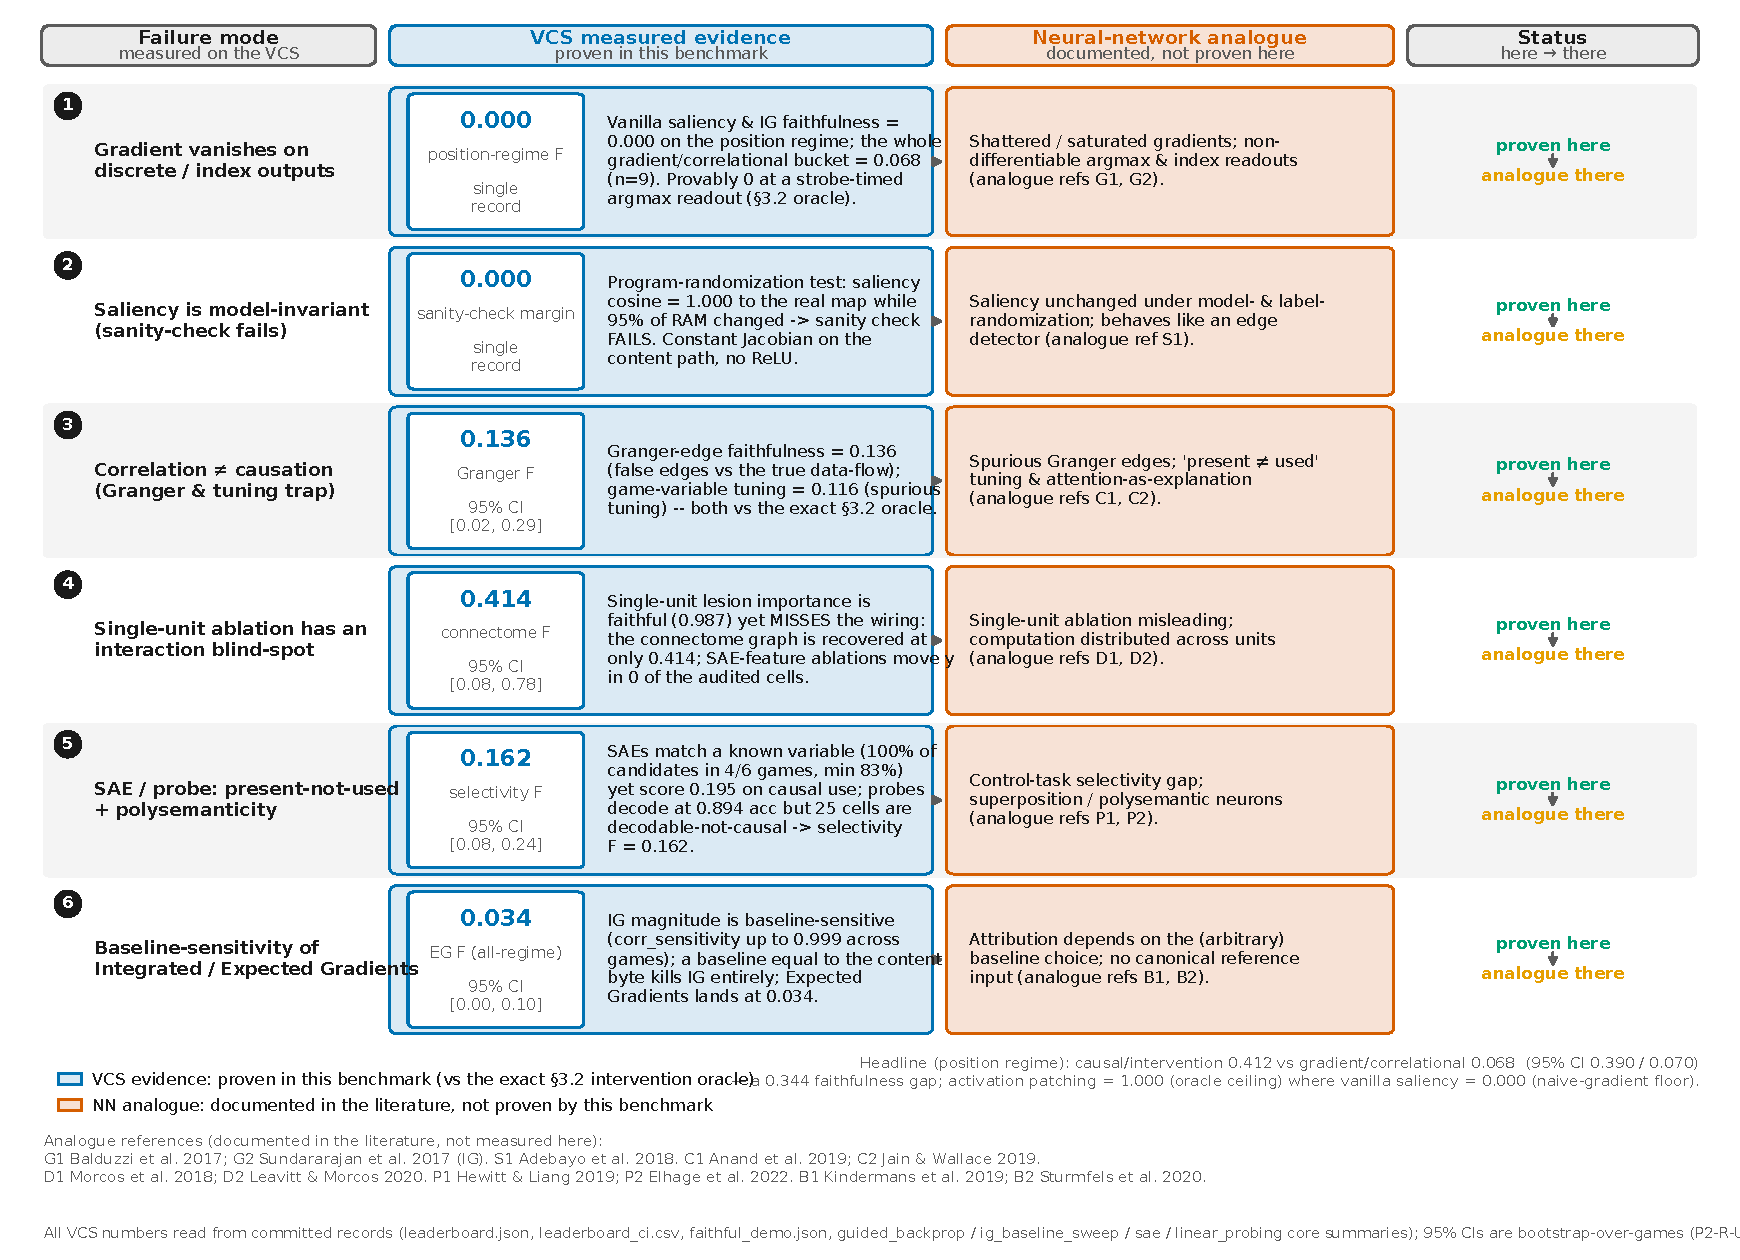
\includegraphics[width=\textwidth]{../figures/fig5_representativeness_map_full.pdf}
\caption{\textbf{Full VCS-to-NN representativeness map.} The full-density version of the
main-text map (Fig.~\ref{fig:representativeness}): each VCS failure mode is placed against its documented
neural-network analogue from the literature. The neural-network column records documented
analogues, not parallels proven by this benchmark; the oracle is the intervention oracle of
\Sectionname3.2, and the underlying per-method values trace to
\texttt{compare/out/leaderboard.json} via Sec.~\ref{supp:provenance}. Note that this full
map is the figure the simplified main-text version condenses.}
\label{supp:fig:repmap}
\end{figure}

\begin{figure}[t]
\centering
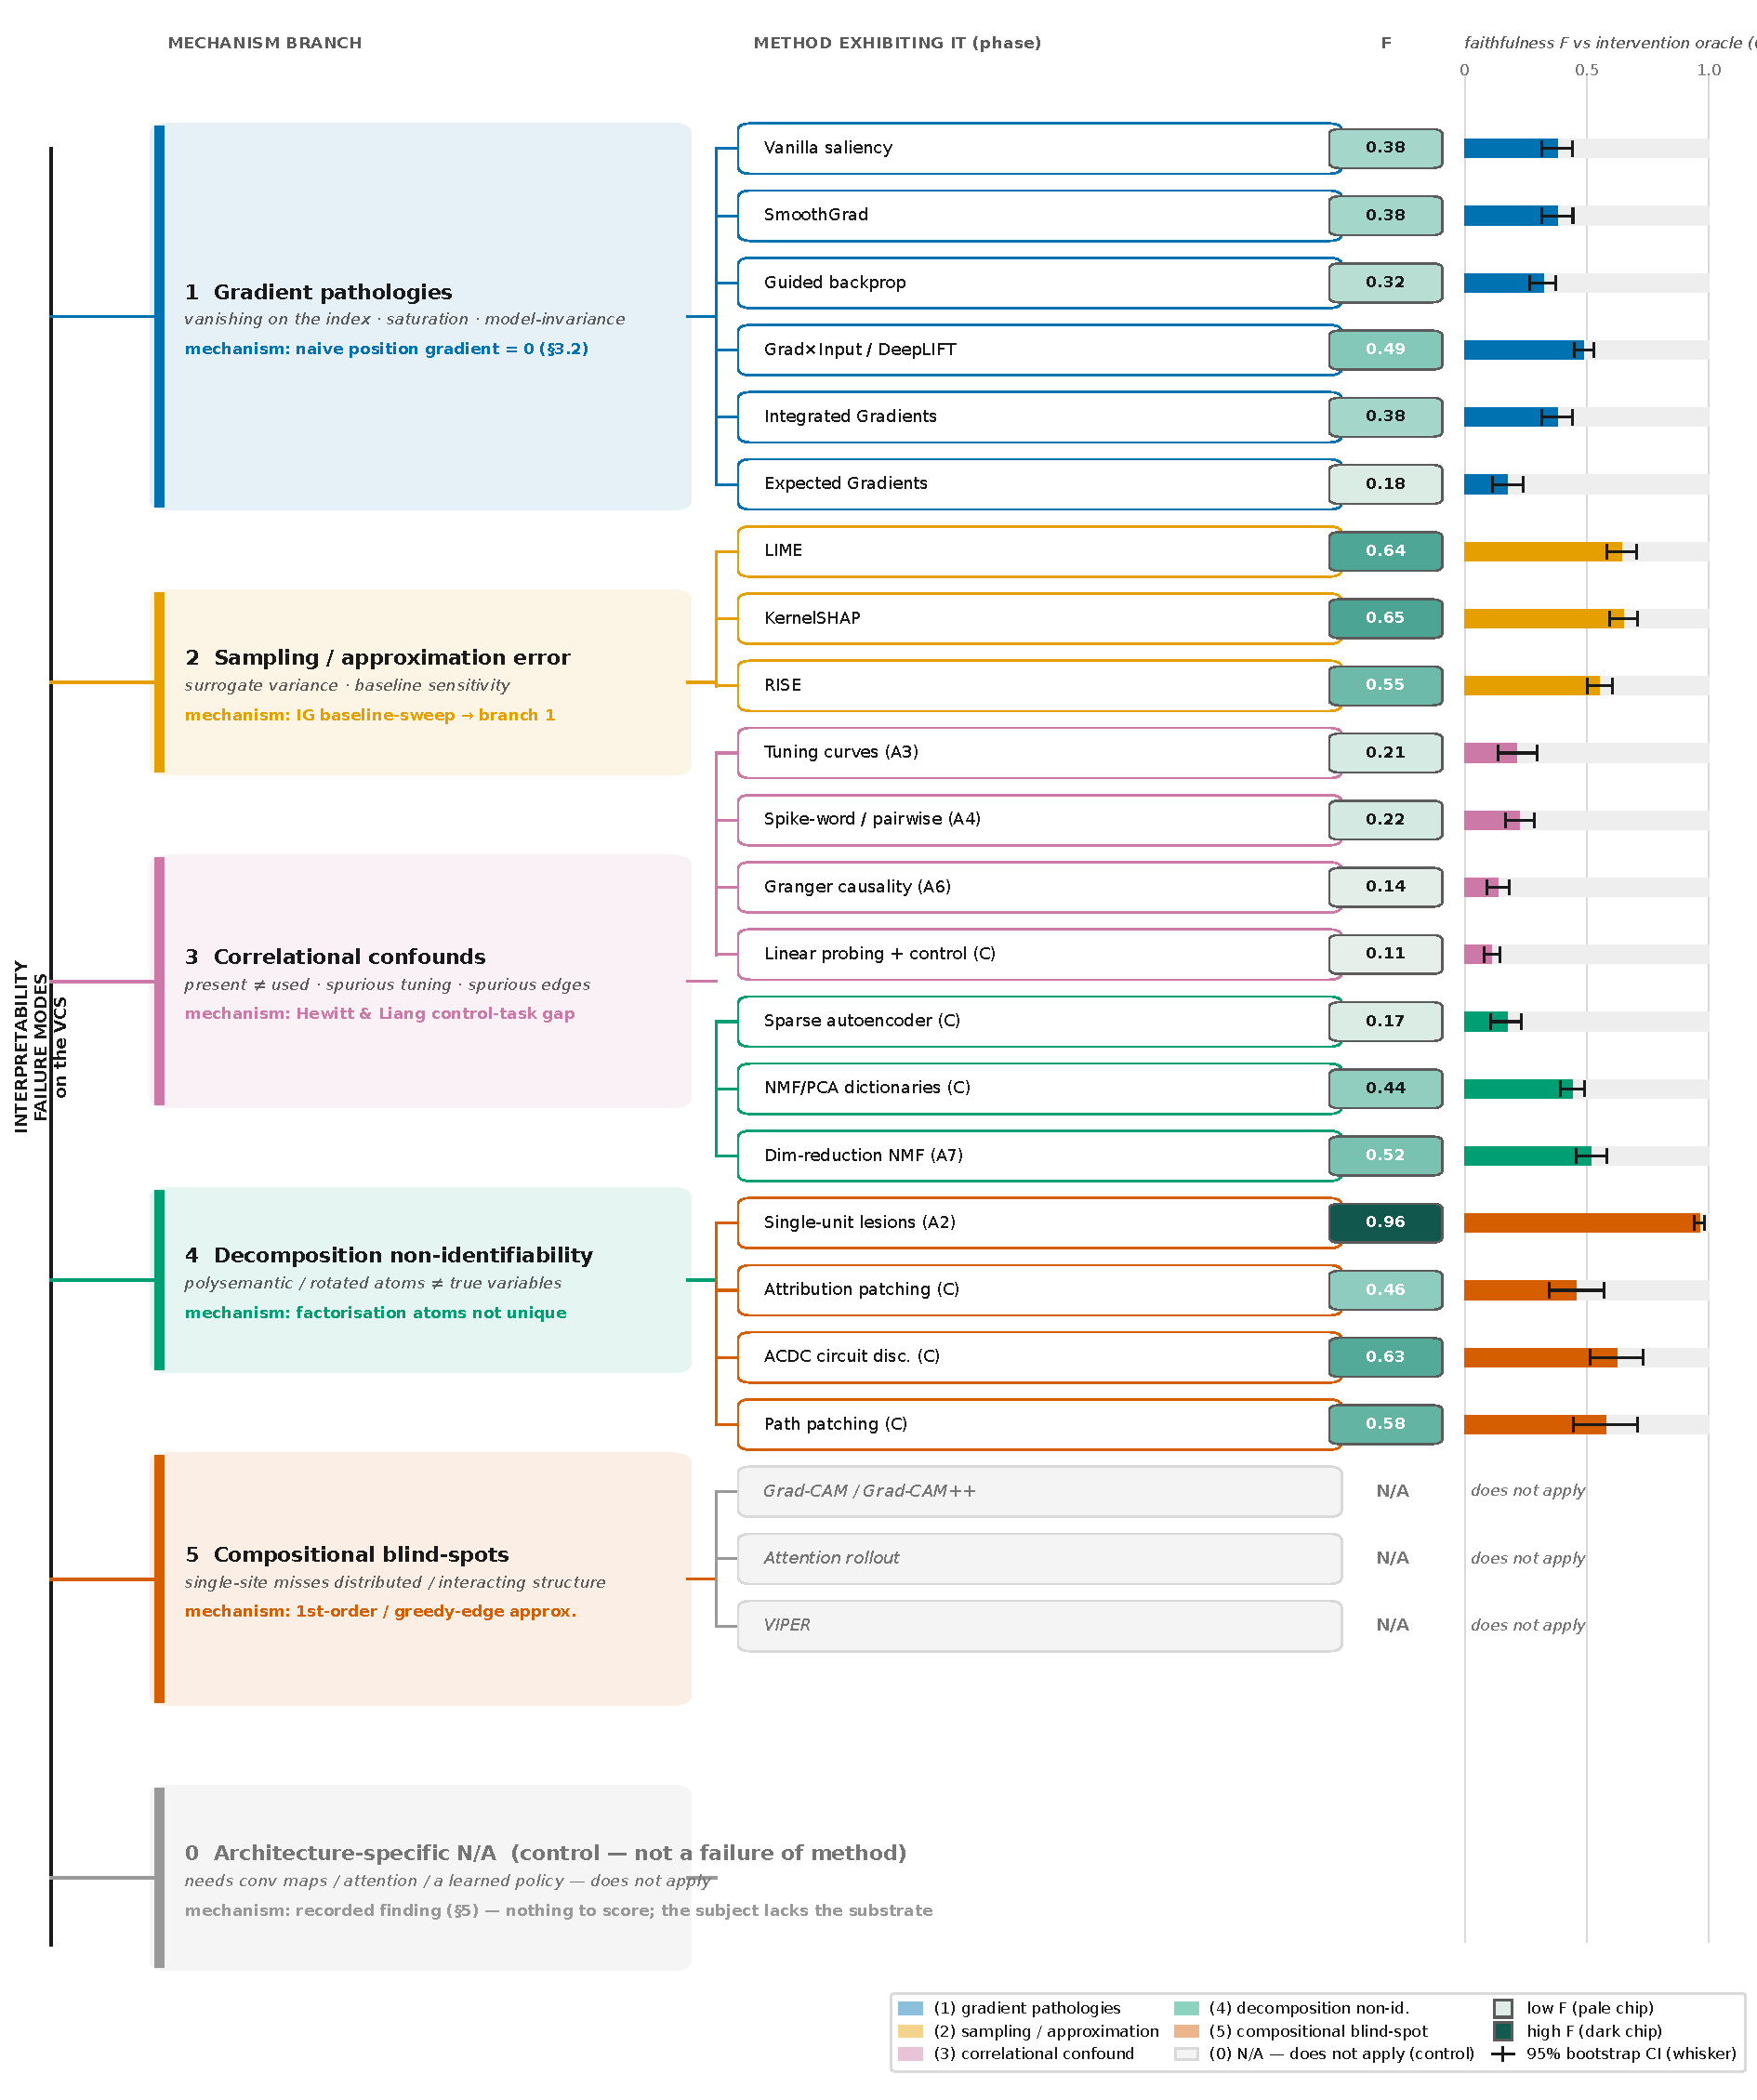
\includegraphics[width=\textwidth]{../figures/fig6_failure_taxonomy_full.pdf}
\caption{\textbf{Full failure taxonomy.} The full-density version of the main-text taxonomy
(Fig.~\ref{fig:taxonomy}): the families of interpretability failure observed on the machine, each annotated
with its faithfulness against the intervention oracle (\Sectionname3.2), reported as $F$ with its
$95\%$ bootstrap confidence interval. The leaf values trace to
\texttt{compare/out/leaderboard.json} and \texttt{leaderboard\_ci.csv} via
Sec.~\ref{supp:provenance}. Note that the gradient and correlational branches collapse on
the discrete position regime, where the naive gradient is provably zero (Prop.~\ref{prop:zero}).}
\label{supp:fig:taxonomy}
\end{figure}

\section{Plausibility-proxy rubric and its sensitivity}\label{supp:plausibility}

The plausibility axis of the leaderboard is a documented, tradition-level proxy, not a
human-subjects measurement. This section records how each value was assigned. It also shows
that the headline contrast does not depend on the particular numbers chosen. The Methods
(\Sectionname\ref{sec:triad}) name two reporting axes. Faithfulness is measured on the machine against the
intervention oracle of \Sectionname\ref{sec:oracle}. The plausibility proxy stands in for how convincing a
tradition's explanations are usually taken to be. We assign the proxy once per method
tradition, before any faithfulness score on our machine is computed, so it cannot be tuned to
the result. Its only job is to expose the danger zone of explanations that look convincing yet
are unfaithful. For that job it must be coarse, fixed in advance, and sourced rather than
precise.

The rubric assigns one proxy per tradition on a fixed five-step scale. It scores two
documented properties of each tradition's typical output and takes their average. The first
property is whether the explanation produces a dense, picture-like artifact that a reader sees
as an account of the computation. Heatmaps and saliency-style maps over the input are read as
convincing by construction. This is the perceptual-immediacy axis. The second property is
whether the field has historically treated the tradition's output as a self-evident
explanation rather than a hypothesis to be tested. This is the adoption-as-explanation axis. A
tradition that scores high on both, such as gradient saliency, receives a high proxy. A
tradition whose output is an austere intervention table or a circuit edge list, rarely
mistaken for a finished story, receives a low one. The scale is deliberately blunt,
$\{0.3,0.5,0.55,0.75,0.8,0.85,0.9\}$. A proxy meant to expose a danger zone gains nothing from
false precision, and a finer scale would invite over-reading. Every value in
Table~\ref{supp:tab:plausrubric} traces to the \jkey{plausibility_proxy} field of the
per-method rows in \texttt{compare/out/leaderboard.json}. The table only groups those rows by
tradition and records the rationale.

\begin{table}[t]
\centering
\caption{\textbf{Plausibility-proxy rubric.} The proxy assigned to each method tradition,
with the documented rationale. Values are the \jkey{plausibility_proxy} field of the
leaderboard rows (\texttt{compare/out/leaderboard.json}). They are tradition-level and fixed
before any faithfulness score is computed, so the proxy cannot be tuned to the measured
faithfulness. A higher value means an explanation that the field tends to find more
convincing, not one that is more faithful. The oracle (\Sectionname\ref{sec:oracle}) is the positive control and
is not a method under test.}
\label{supp:tab:plausrubric}
\begin{tabular}{@{}llp{6.4cm}@{}}
\toprule
Tradition & Proxy & Rationale (documented basis) \\
\midrule
gradient        & $0.90$ & Dense input-space heatmaps read as a visual account of the
                            decision; the most widely adopted XAI outputs, routinely shown
                            as if self-explanatory. \\
probing         & $0.85$ & A trained decoder that ``finds'' a concept reads as evidence the
                            concept is used; high adoption, though decodability is not
                            causal use. \\
correlational   & $0.80$ & Tuning curves and coupling spectra match the neuroscience idiom
                            of a convincing single-unit account. \\
dim.\ reduction & $0.75$ & Low-dimensional factors and dictionary atoms look like a clean
                            summary of the representation. \\
intervention    & $0.55$ & Occlusion and counterfactual outputs are quantitative tables, less
                            immediately picture-like, treated as tests rather than stories. \\
causal          & $0.50$ & Circuit edge lists and patching results are austere artifacts
                            rarely mistaken for a finished narrative. \\
descriptive     & $0.30$ & Whole-state recording is an explicit non-explanation: it withholds
                            nothing and reads as a dump, not an account. \\
\midrule
oracle (control)& $1.00$ & The \Sectionname\ref{sec:oracle} ground truth by construction; positive control, not a
                            method under test. \\
\bottomrule
\end{tabular}
\end{table}

The paper draws a contrast between this proxy and measured faithfulness. On the committed
records the two move in opposite directions. Across the thirty methods under test the Spearman
rank correlation between faithfulness and the proxy is $-0.36$, a negative association.
The traditions the field finds most convincing are, on this machine, among the least faithful.
Eight methods fall in the danger zone, defined here as a proxy of at least $0.70$ together
with a faithfulness below $0.40$. They include the correlational neuroscience methods, Expected
Gradients, guided backprop, linear probing, and the sparse autoencoder. The per-method extreme
makes the point sharply. Vanilla saliency has the highest proxy, $0.9$, yet scores faithfulness
$0.115$ on the position regime. Activation patching has a lower proxy, $0.5$, and scores $1.0$.
Here the less faithful method is the more plausible one. These figures are produced by
\texttt{tools/xai\_study/compare/plausibility\_sensitivity.py} from the leaderboard and
recorded in \texttt{compare/out/plausibility\_sensitivity.csv}.

A proxy fixed by a coarse rubric raises the question of whether the contrast is an artifact of
the particular numbers. The answer is that it is not. We perturb the proxy under four
deterministic schemes and recompute the relationship each time. The analysis uses fixed,
index-keyed offsets rather than random draws, so it re-derives bit-for-bit. The first scheme
adds a fixed per-method jitter of magnitude $\sigma\in\{0.05,0.1,0.2\}$, alternating in sign by
row. The second compresses every proxy toward the common mean by a fraction $\sigma$, which
preserves the rank order of traditions. The third uses the same index-keyed offsets at
$\sigma\in\{0.1,0.2\}$, large enough to swap neighbouring traditions' ranks. The fourth drops
one whole tradition at a time and recomputes on the remainder. Across all fourteen
perturbations the rank correlation between faithfulness and proxy stays negative. It ranges
from $-0.76$ to $-0.08$. The danger zone stays populated, with
between four and ten methods. The per-method anchor sign holds in every scheme where both
anchor methods are present, the more plausible saliency remaining the less faithful. Two runs
bound the range. The strongest is the leave-the-gradient-tradition-out run. It removes the most
plausible and least faithful block at once, and still leaves six danger-zone methods and a rank
correlation of $-0.76$. The weakest is the leave-the-causal-tradition-out run, where the
correlation falls to $-0.08$, close to zero; removing the faithful causal block flattens the
association, so the contrast is carried in part by that block. Table~\ref{supp:tab:plaussens}
reports the full sweep. The contrast keeps its sign under every alternative proxy assignment we
tried: plausibility and faithfulness are not the same axis, and high plausibility is no
guarantee of faithfulness.

\begin{table}[t]
\centering
\caption{\textbf{Proxy-sensitivity sweep.} The faithfulness-versus-proxy relationship under
each perturbation, from \texttt{compare/out/plausibility\_sensitivity.csv}. ``$\rho$'' is the
Spearman rank correlation between faithfulness and proxy over the methods present. ``danger''
is the count of high-proxy ($\geq0.70$), low-faithfulness ($<0.40$) methods. ``anchor'' is
$1$ when the more plausible saliency is the less faithful of the saliency/activation-patching
pair, and blank where a leave-one-out run removes an anchor. The baseline rubric is the first
row. Across every scheme the correlation stays negative and the danger zone stays populated.}
\label{supp:tab:plaussens}
\begin{tabular}{@{}llrrrc@{}}
\toprule
Scheme & Param & $n$ & $\rho$ & Danger & Anchor \\
\midrule
baseline                & ---           & 30 & $-0.36$ &  8 & 1 \\
additive jitter         & $\sigma=0.05$ & 30 & $-0.40$ &  8 & 1 \\
additive jitter         & $\sigma=0.10$ & 30 & $-0.41$ &  8 & 1 \\
additive jitter         & $\sigma=0.20$ & 30 & $-0.42$ & 10 & 1 \\
rank-preserving         & $\sigma=0.10$ & 30 & $-0.36$ &  8 & 1 \\
rank-preserving         & $\sigma=0.20$ & 30 & $-0.36$ &  8 & 1 \\
rank-jittering          & $\sigma=0.10$ & 30 & $-0.41$ &  8 & 1 \\
rank-jittering          & $\sigma=0.20$ & 30 & $-0.42$ & 10 & 1 \\
leave-out causal        & ---           & 24 & $-0.08$ &  8 & \\
leave-out correlational & ---           & 26 & $-0.40$ &  4 & 1 \\
leave-out descriptive   & ---           & 29 & $-0.29$ &  8 & 1 \\
leave-out dim.\ red.    & ---           & 27 & $-0.34$ &  7 & 1 \\
leave-out gradient      & ---           & 20 & $-0.76$ &  6 & \\
leave-out intervention  & ---           & 25 & $-0.34$ &  8 & 1 \\
leave-out probing       & ---           & 29 & $-0.36$ &  7 & 1 \\
\bottomrule
\end{tabular}
\end{table}



\end{document}
